\documentclass{beamer}
\usepackage{appendixnumberbeamer}
\usepackage{tikz}
\usepackage{calc}
\usepackage{subcaption}
\usepackage{siunitx}
\usepackage{booktabs}

\usetheme{Hannover}
\usecolortheme[RGB={0 35 102}]{structure} % Set our primary color
\setbeamertemplate{navigation symbols}{} % Disable the navigation buttons

% Fixes warning. See https://tex.stackexchange.com/a/330980.
\pdfstringdefDisableCommands{
  \def\translate{}
}

% Define command that creates a presenter box
\newlength{\presenterboxwidth}
\newcommand{\presenterbox}[2]{
    \ifdefined\presentertextbox
    \else
        \newsavebox{\presentertextbox}
    \fi
    \sbox{\presentertextbox}{#1, #2}
    \pgfmathsetlength{\presenterboxwidth}{\wd\presentertextbox + 7.5}
    \begin{tikzpicture}
        \usebeamercolor{sidebar}
        \fill[fill=bg] (0, 0) -- (\presenterboxwidth + 15, 0) -- (\presenterboxwidth, 0.5) -- (0, 0.5) -- cycle;
        \usebeamercolor{title in sidebar}
        \node[anchor=west, font=\tiny, text=fg] at (0.05, 0.25) {#1, #2};
    \end{tikzpicture}
}

% These commands set the presenter name and title to use in the footer
\newcommand{\setpresentername}[1]{\renewcommand{\presentername}{#1}}
\newcommand{\setpresentertitle}[1]{\renewcommand{\presentertitle}{#1}}
\newcommand{\presentername}{}
\newcommand{\presentertitle}{}

% This command determines whether the presenter box footer is displayed:
\newif\ifshowpresenterbox
\showpresenterboxtrue

% This command determines whether the headline is displayed:
\newif\ifshowheadline
\showheadlinetrue

% Get the width of the sidebar
\makeatletter
\newlength{\sidebarwidth}
\setlength{\sidebarwidth}{\beamer@sidebarwidth}
\makeatother

% Add slide number to the headline
\setbeamertemplate{headline}{
    \ifshowheadline
        \hfill
        \insertframenumber{} / \inserttotalframenumber
        \hspace*{5pt}
        \vspace*{-12pt}
    \fi
}

% Add the presenter name and job title to the footer
\setbeamertemplate{footline}{
    \ifshowpresenterbox
        \vspace{-50pt}
        \hspace{\sidebarwidth - 6.75pt}
        \presenterbox{\presentername}{\presentertitle}
    \fi
}

\title[Conceptual Design Review]{Conceptual Design Review Presentation}
\subtitle{The Banshee}
\author{StratoShield}
\institute{Iowa State University}
\date{Tuesday, November 5\textsuperscript{th}, 2024}

\begin{document}
    \showpresenterboxfalse
    \begin{frame}
        \titlepage
    \end{frame}
    \showpresenterboxtrue

    \section{Introduction}
    
    \setpresentername{Matthew Mehrtens}
    \setpresentertitle{Project Manager}
    
    \begin{frame}
        \centering
        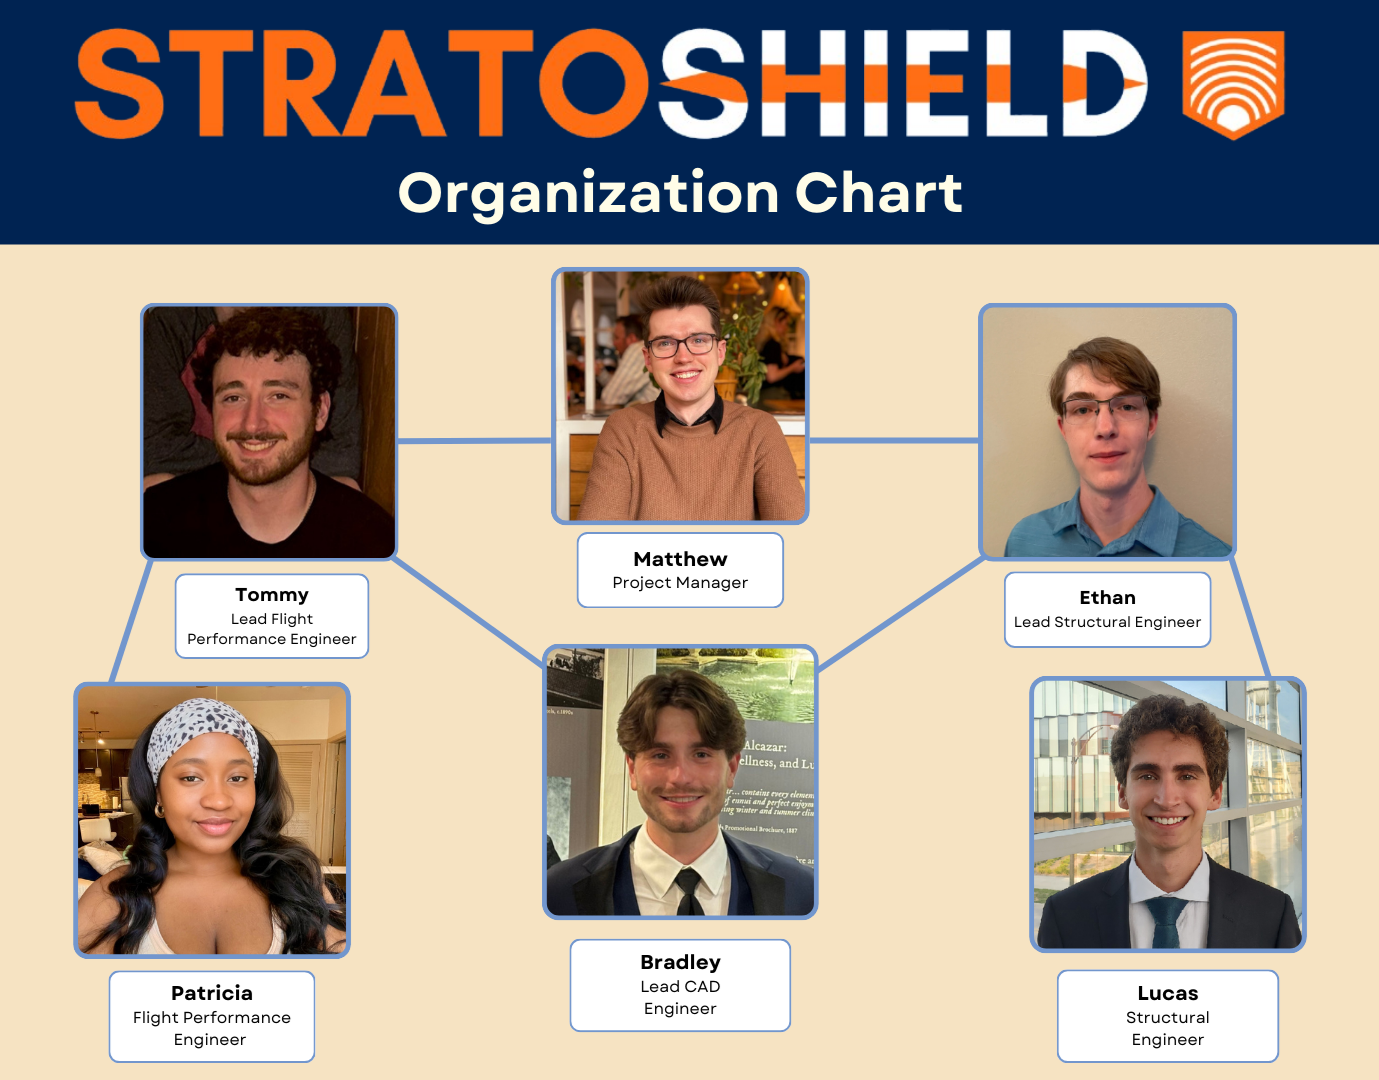
\includegraphics[width=\linewidth]{figures/StratoShield Organization Chart v1.1.0.png}
    \end{frame}
    
    \begin{frame}{Executive Summary}
        \tableofcontents
    \end{frame}
    
    \section{Mission and Requirements}

    \begin{frame}{Mission}
        \begin{itemize}
            \item Customer: Department of Homeland Security
            \item Mission: Protect U.S. citizens from hostile sUAS
        \end{itemize}
    \end{frame}

    \begin{frame}{Threats Posed by sUAS}
        \begin{itemize}
            \item<1-> Surveillance and espionage
            \item<2-> Smuggling payloads
            \item<3-> GPS spoofing and jamming
            \item<4-> Weaponization
        \end{itemize}
    \end{frame}

    \begin{frame}{Key Requirements}
        \centering
        \begin{enumerate}
            \item<1->The UAV shall prevent a hostile airborne sUAS from reaching a key area in an AOI where the key area is at most a circular area of $\approx\qty{100}{acres}$.
            \item<2->The UAV shall be capable of detecting an airborne sUAS.
            \item<3->The UAV shall be capable of fixed-wing flight.
            \item<4->The UAV shall support autonomous flight.
        \end{enumerate}
        \centering
        \vspace{-50pt}
        \includegraphics<1>[width=0.7\linewidth]{figures/aoi.png}
    \end{frame}

    \begin{frame}{Solutions}
        \centering
        \begin{columns}
            \begin{column}{0.5\textwidth}
                \centering
                Kinetic Impact
                
                \vspace{10pt}
                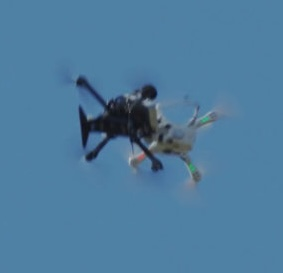
\includegraphics[width=\textwidth]{figures/anduril_anvil.jpg}
            \end{column}
            \begin{column}{0.5\textwidth}
                \centering
                Jamming
                
                \vspace{10pt}
                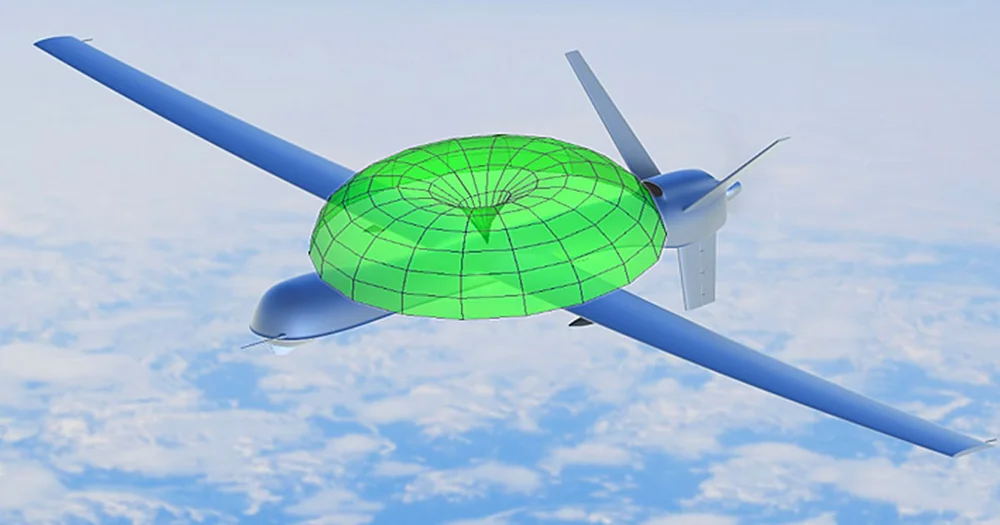
\includegraphics[width=\textwidth]{figures/jamming_uav.png}
            \end{column}
        \end{columns}
    \end{frame}

    \begin{frame}{Mission Profile}
        \centering
        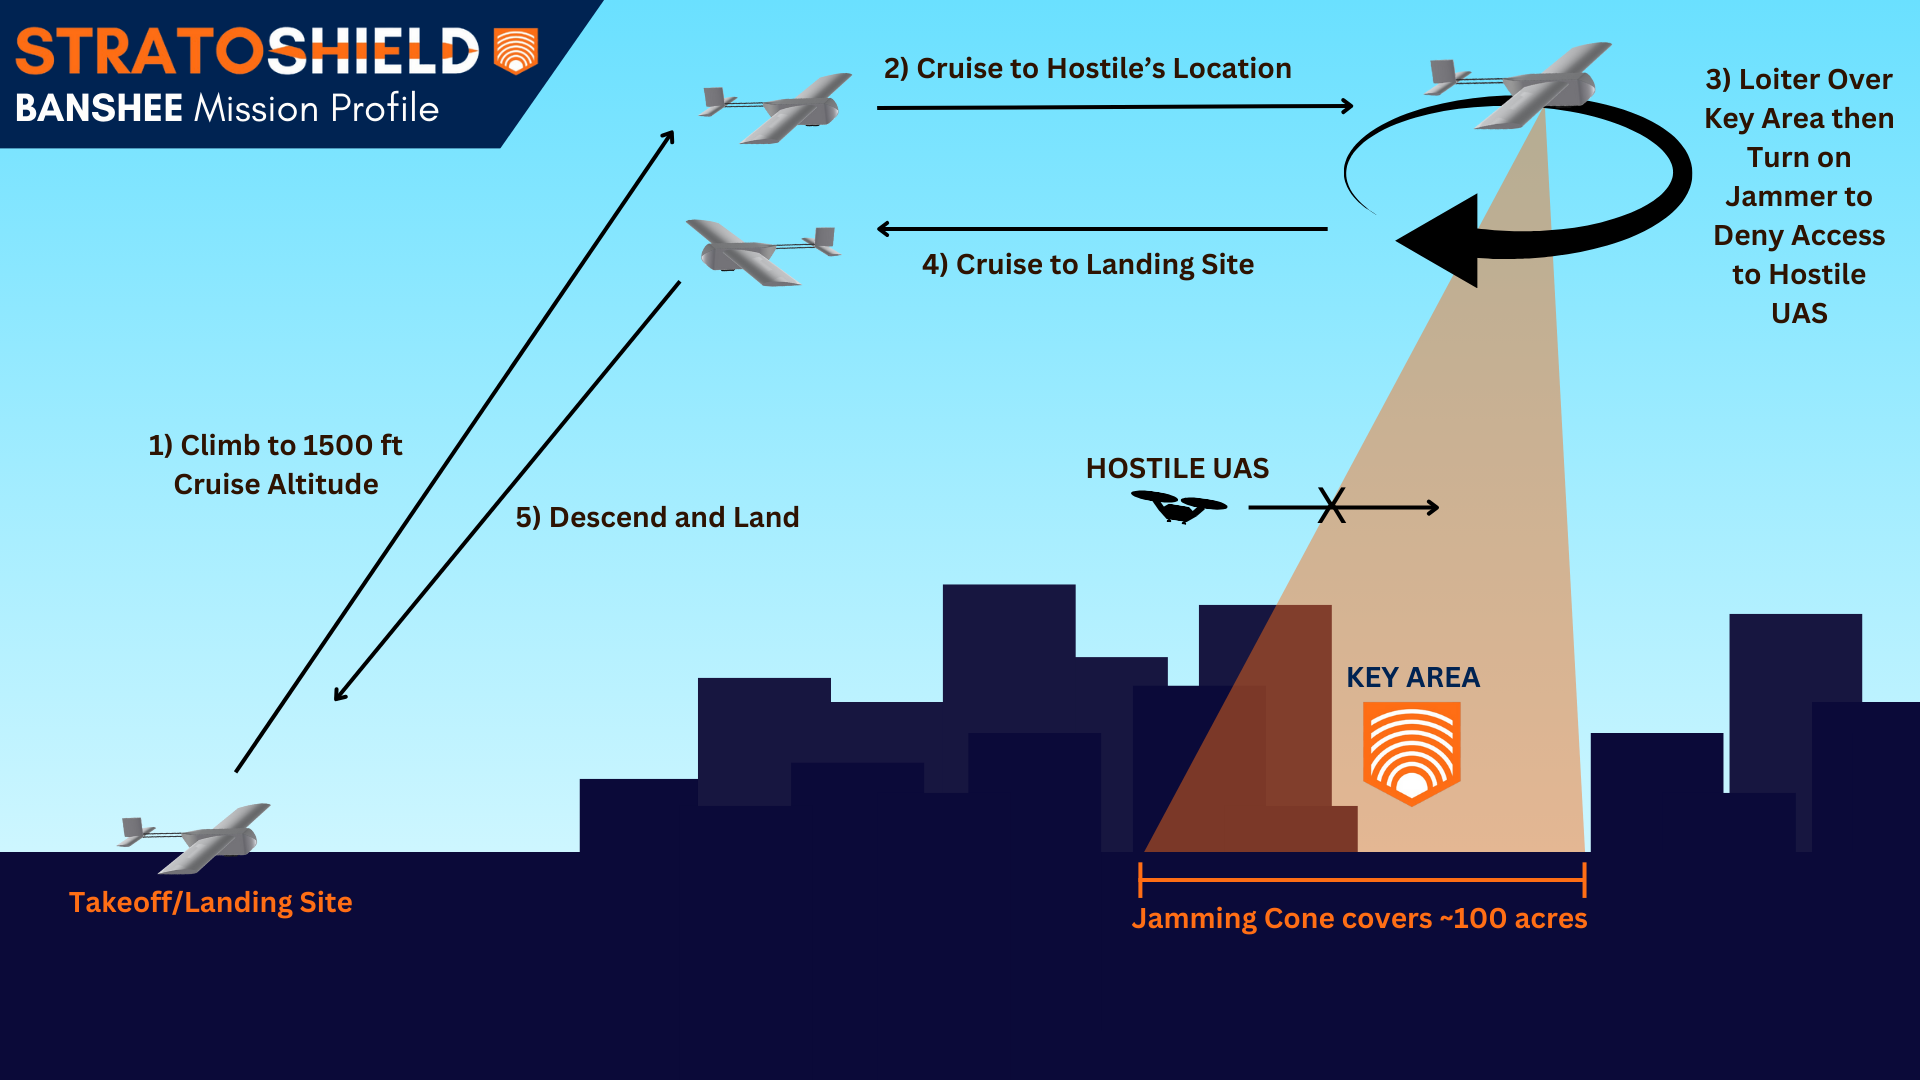
\includegraphics[width=\textwidth]{figures/Mission Profile BANSHEE updated.png}
    \end{frame}

    \section{Market Survey}

    \setpresentername{Bradley Nordwall}
    \setpresentertitle{Lead CAD Engineer}
    
    \begin{frame}{Comparable sUAV}
        \begin{columns}[T]
        \begin{column}{0.5\textwidth}
            \centering
            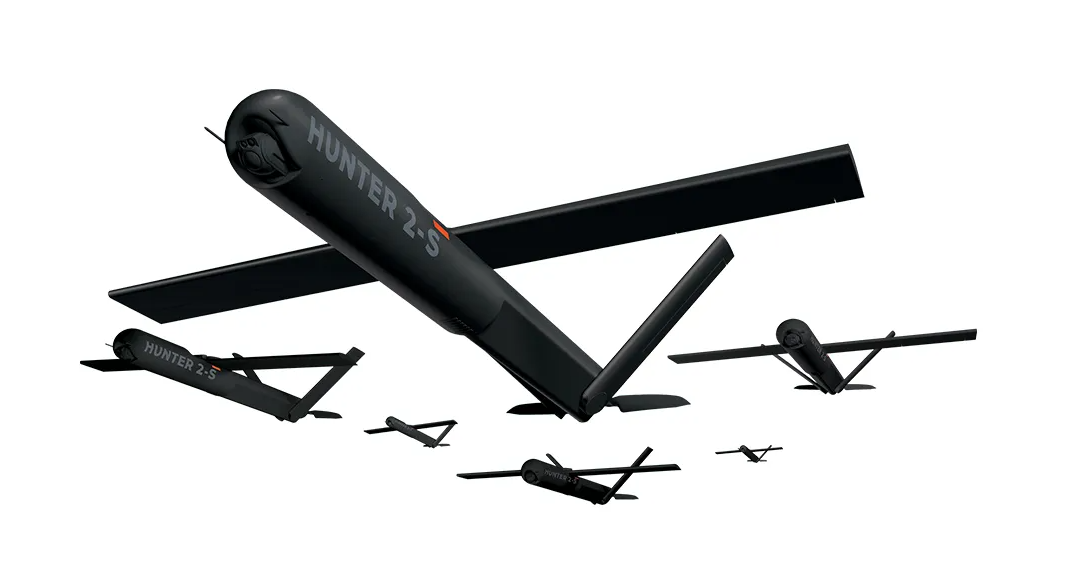
\includegraphics[width=.9\linewidth]{figures/market research/Hunter2S.png}
            \vspace{0.5em} % Space between image and caption
            \text{Hunter 2-S}
        \end{column}
        \begin{column}{0.5\textwidth}
            \centering
            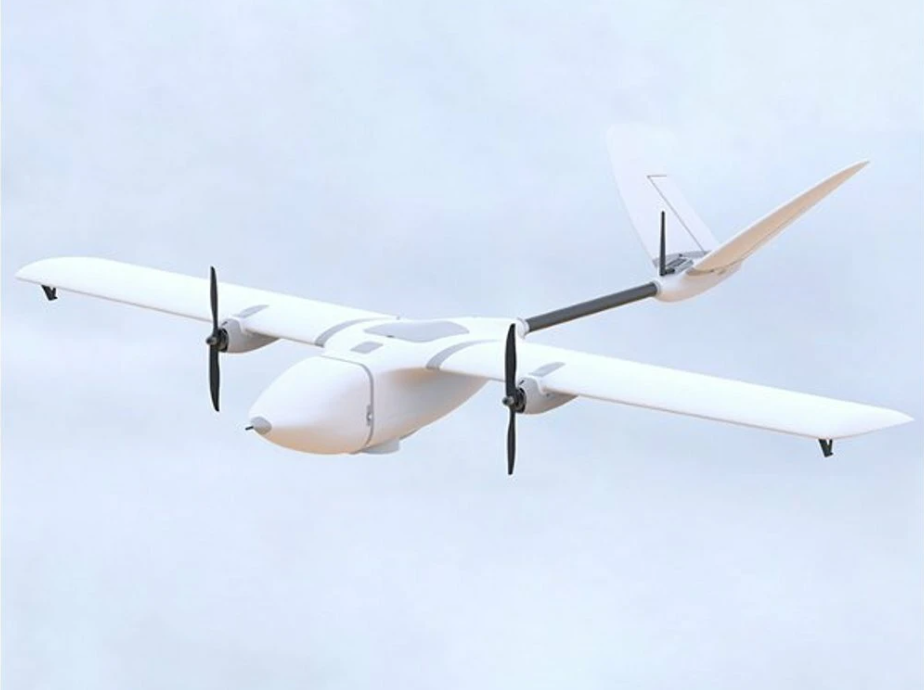
\includegraphics[width=0.65\linewidth]{figures/market research/MFDNimbus.png}
            \vspace{0.5em}
            \text{MyFlyDream Nimbus}
        \end{column}
        \end{columns}
        \vspace{.25em}
        \centering
        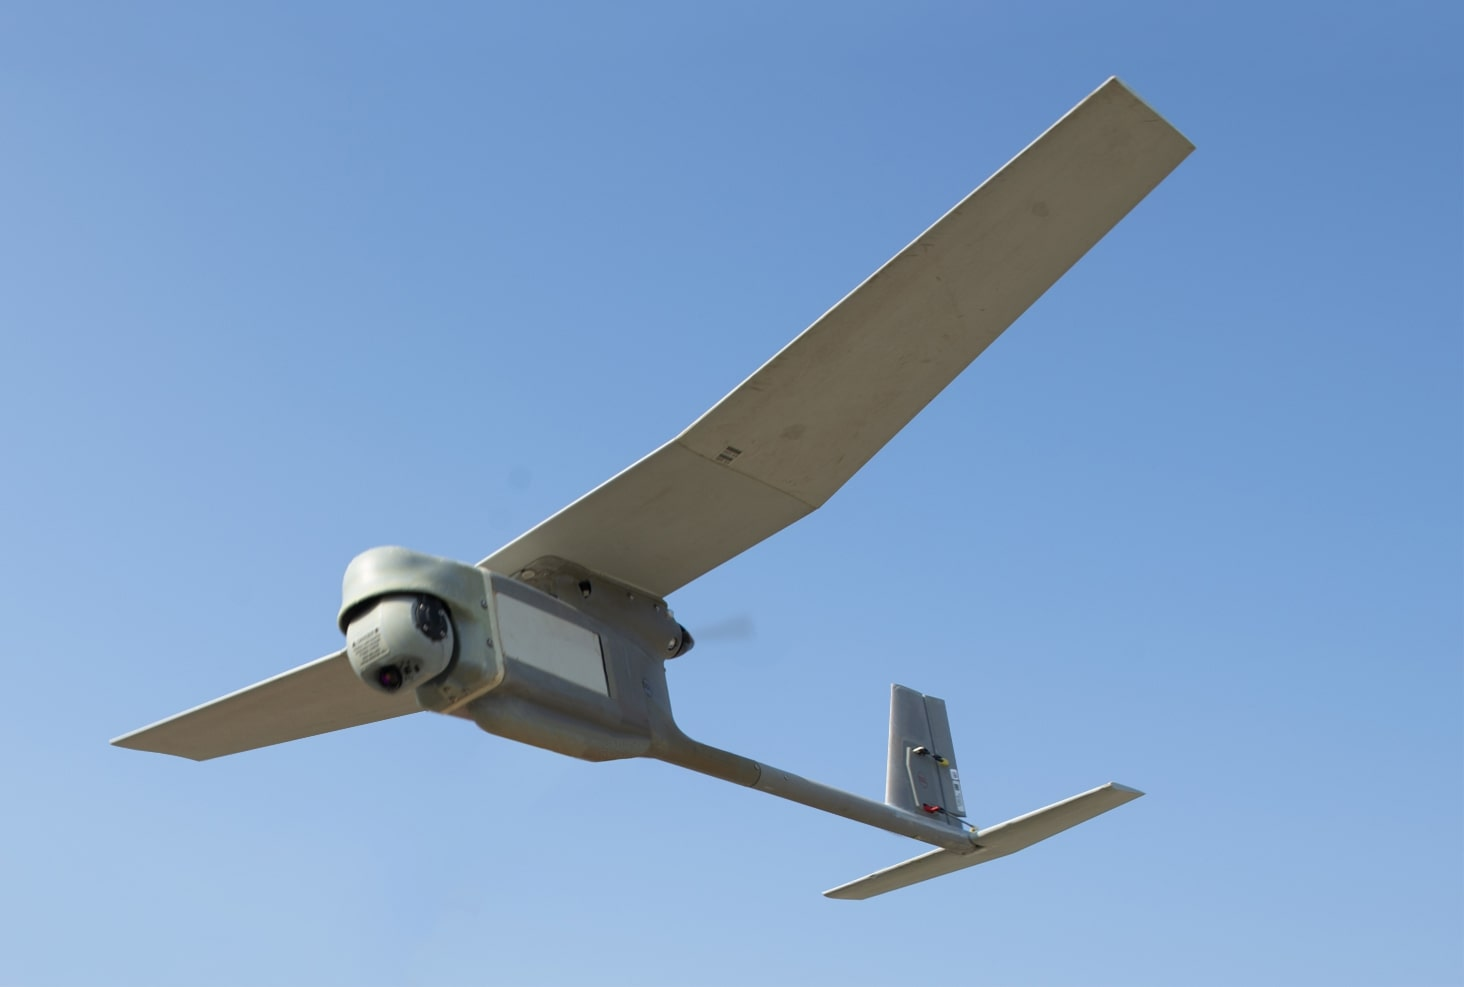
\includegraphics[width=0.35\linewidth]{figures/market research/RQ11Raven.jpg}
        \par
        AeroVironment RQ-11 Raven
    \end{frame}
    
    \begin{frame}
        \centering
        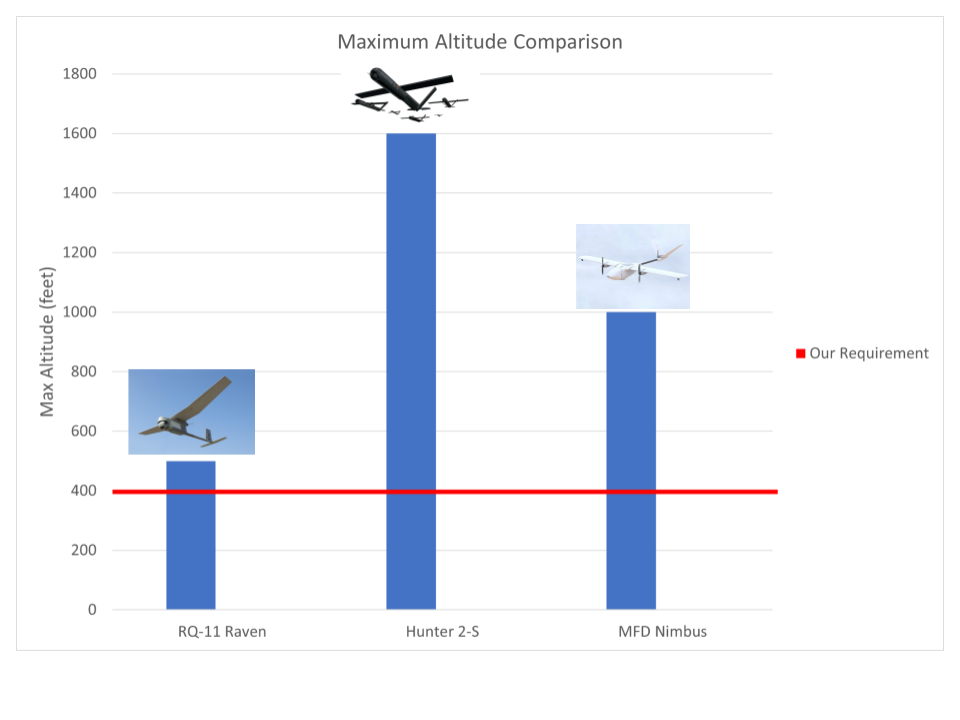
\includegraphics[width=\textwidth]{figures/market research/AltitudeComparison.png}
    \end{frame}
    \begin{frame}
        \centering
        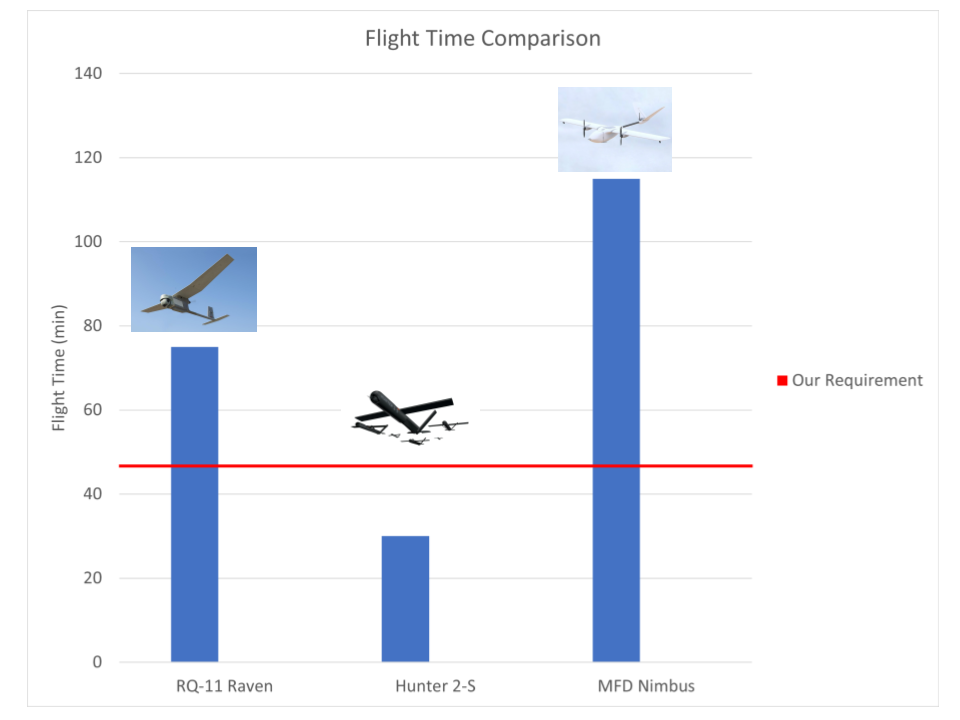
\includegraphics[width=0.9\textwidth]{figures/market research/FlightTimeComparison.png}
    \end{frame}
    \begin{frame}
        \centering
        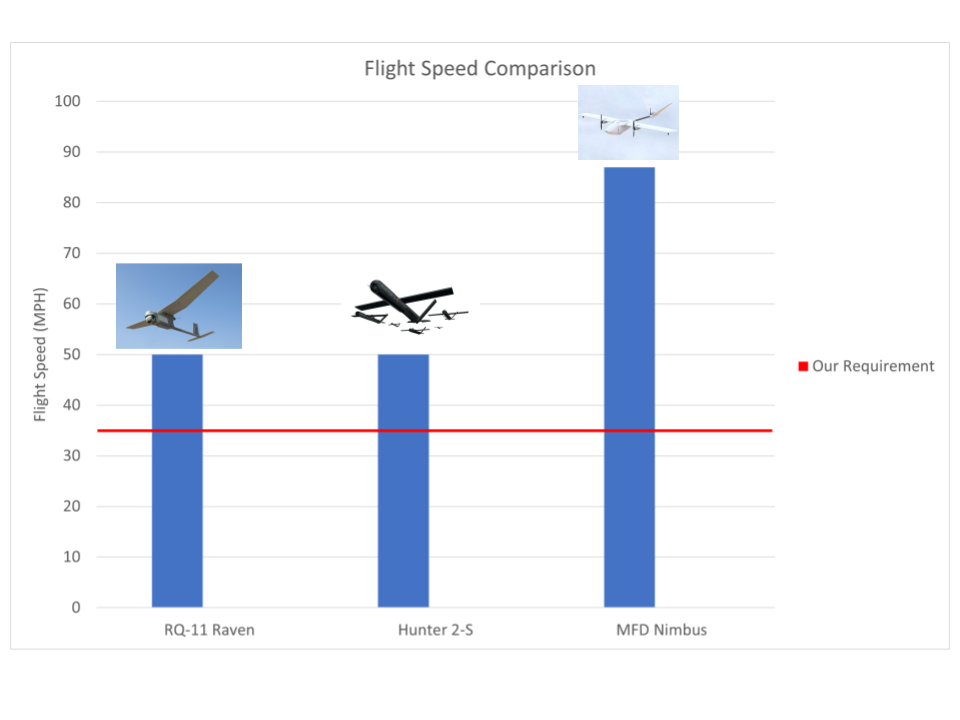
\includegraphics[width=\textwidth]{figures/market research/FlightSpeedComparison.png}
    \end{frame}

    \begin{frame}{Technologies I}
    \begin{columns}
        % Left column for the first image
        \begin{column}{0.5\textwidth}
            \centering
            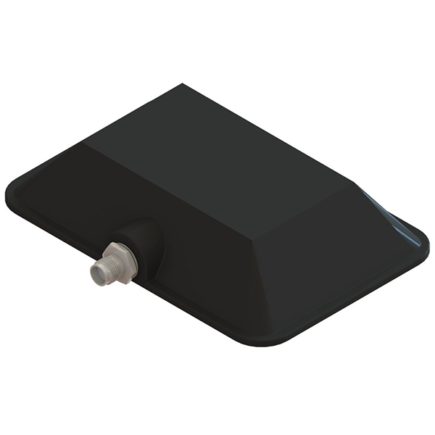
\includegraphics[width=.667\textwidth]{figures/market research/JammingAntenna.png} % Replace with your image path
            \vspace{0.49em} % Space between image and caption
            \text{Jamming Antenna} % Description below the first image
        \end{column}

        % Right column for the second image
        \begin{column}{0.5\textwidth}
            \centering
            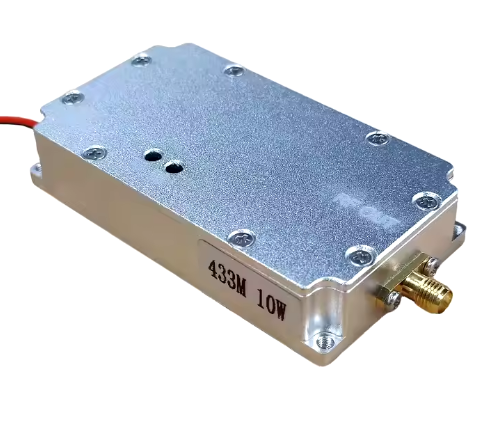
\includegraphics[width=.75\textwidth]{figures/market research/JammingModule.png} % Replace with your image path
            \vspace{0.5em} % Space between image and caption
            \text{Jamming Module} % Description below the second image
        \end{column}
    \end{columns}
    \centering
    \vspace{0.5em}
    Total Weight = \qty{0.50}{lbs}
    \end{frame}

    \begin{frame}{Technologies II}
    \begin{columns}
        % Left column for the first image
        \begin{column}{0.5\textwidth}
            \centering
            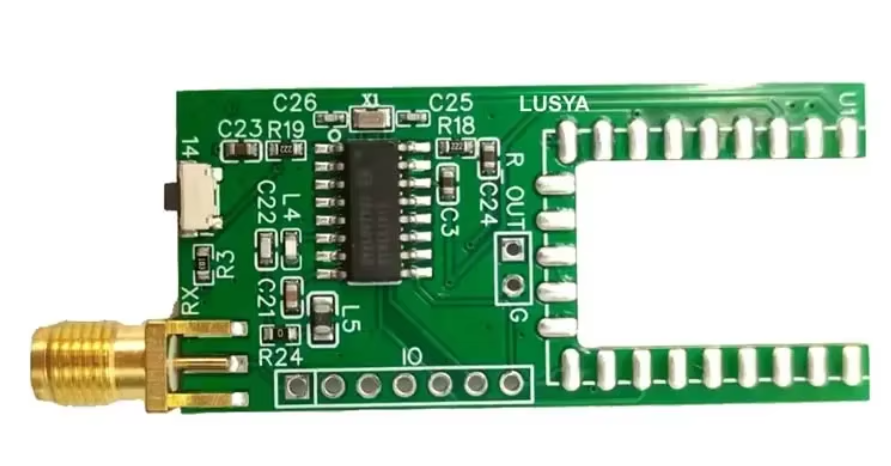
\includegraphics[width=.782\textwidth]{figures/market research/RadioReciever.png} % Replace with your image path
            \vspace{0.5em} % Space between image and caption
            \text{Drone Detector SDR} % Description below the first image
        \end{column}

        % Right column for the second image
        \begin{column}{0.5\textwidth}
            \centering
            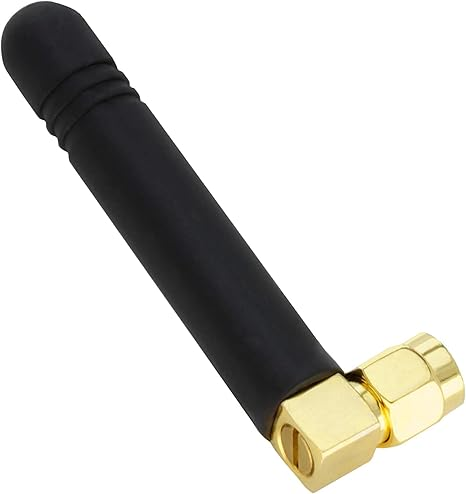
\includegraphics[width=.39\textwidth]{figures/market research/DroneDetectorAntenna.jpg} % Replace with your image path
            \vspace{0.5em} % Space between image and caption
            \text{    Detector Antenna    } % Description below the second image
        \end{column}
    \end{columns}
    \centering
    \vspace{0.5em}
    Total Weight = \qty{0.23}{lbs}
    \end{frame}

    \section{Initial Design}

    \begin{frame}{Initial Design I}
        \centering
        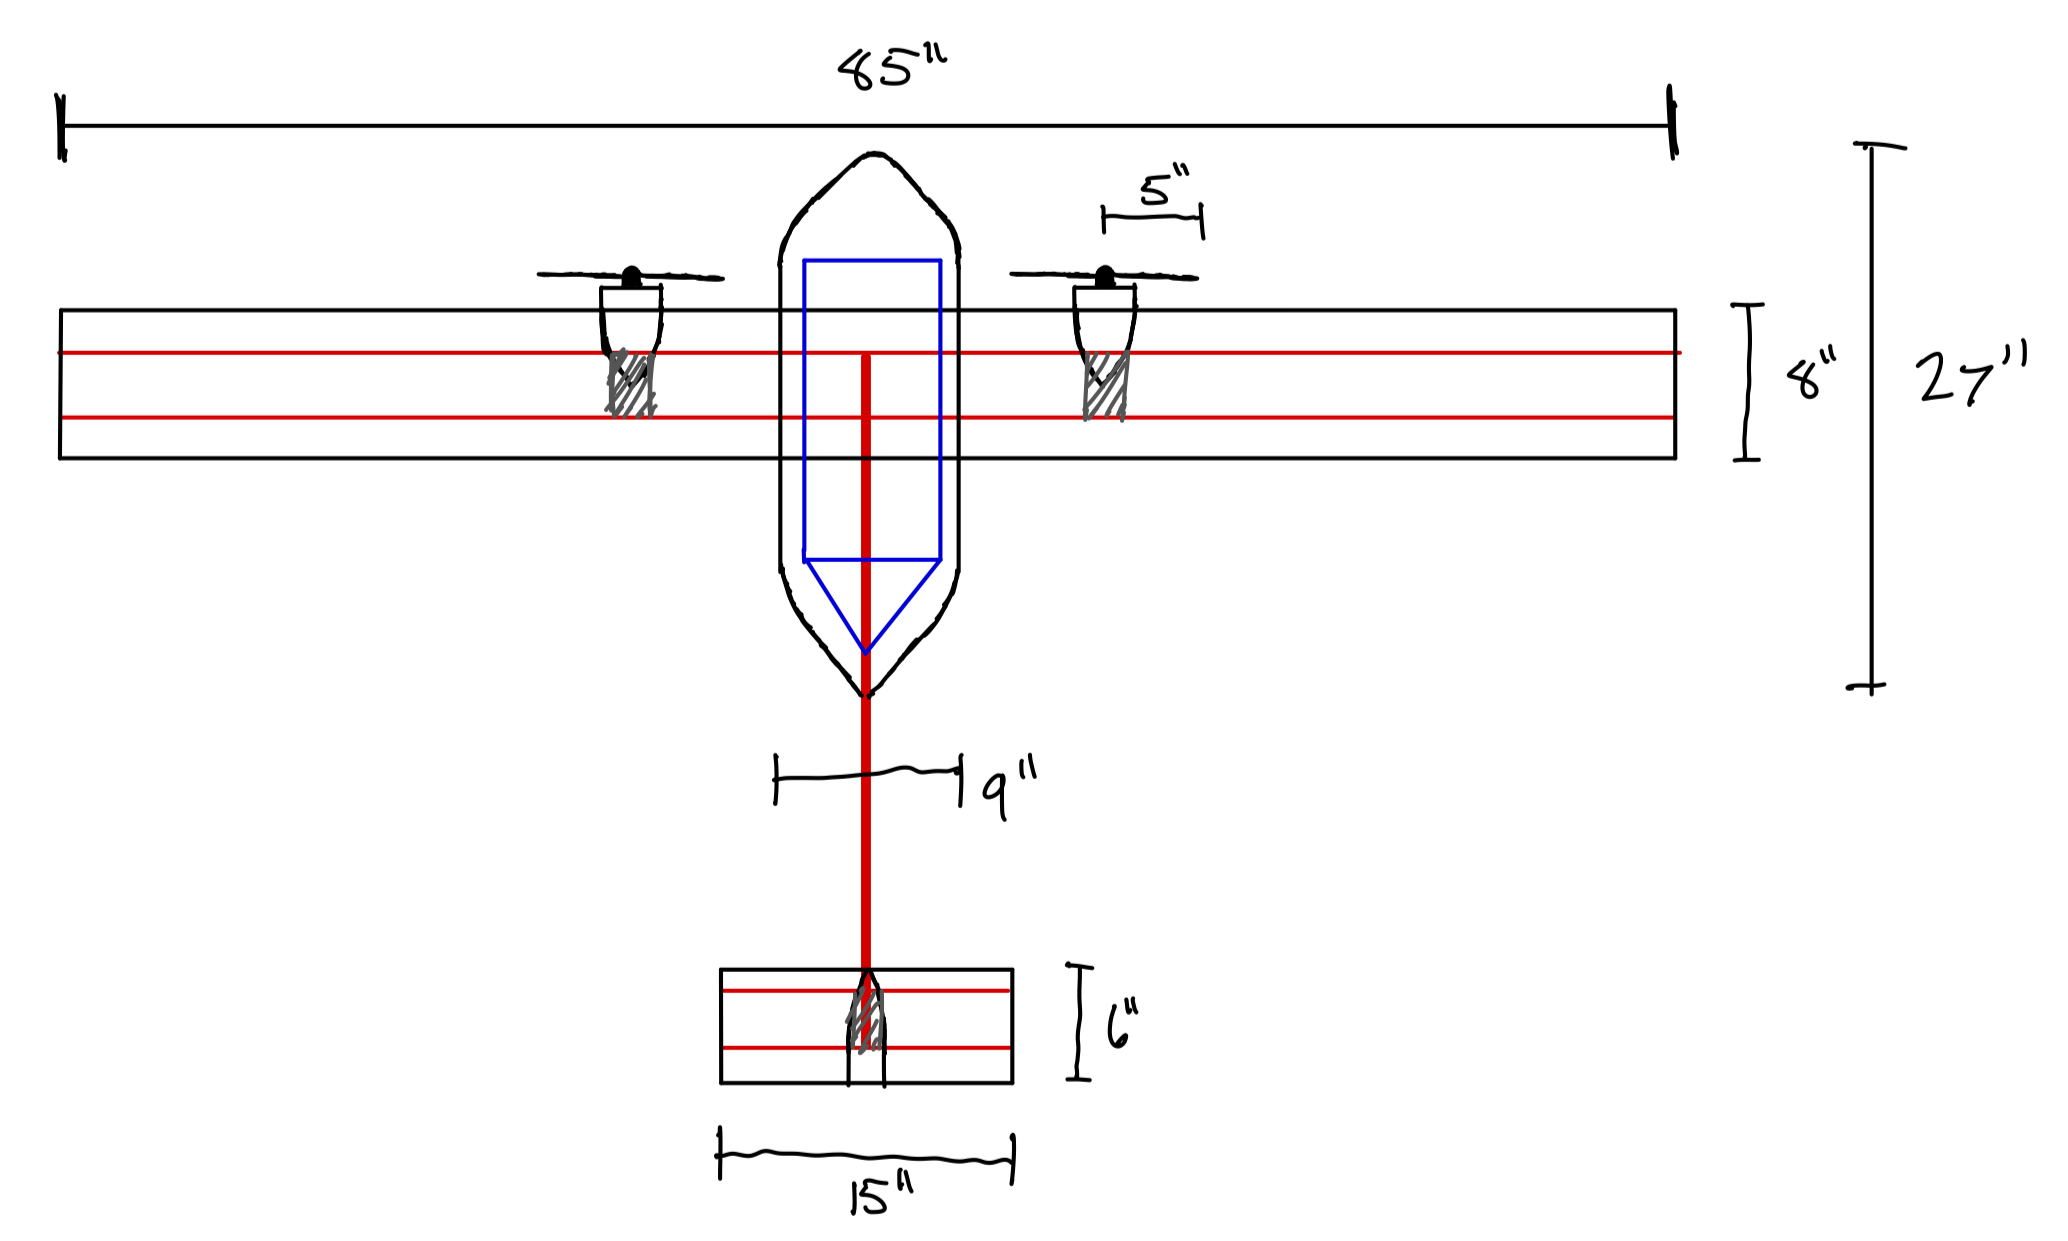
\includegraphics[width=\linewidth]{figures/Initial Design 1.jpeg}
    \end{frame}

    \begin{frame}{Initial Design II}
        \centering
        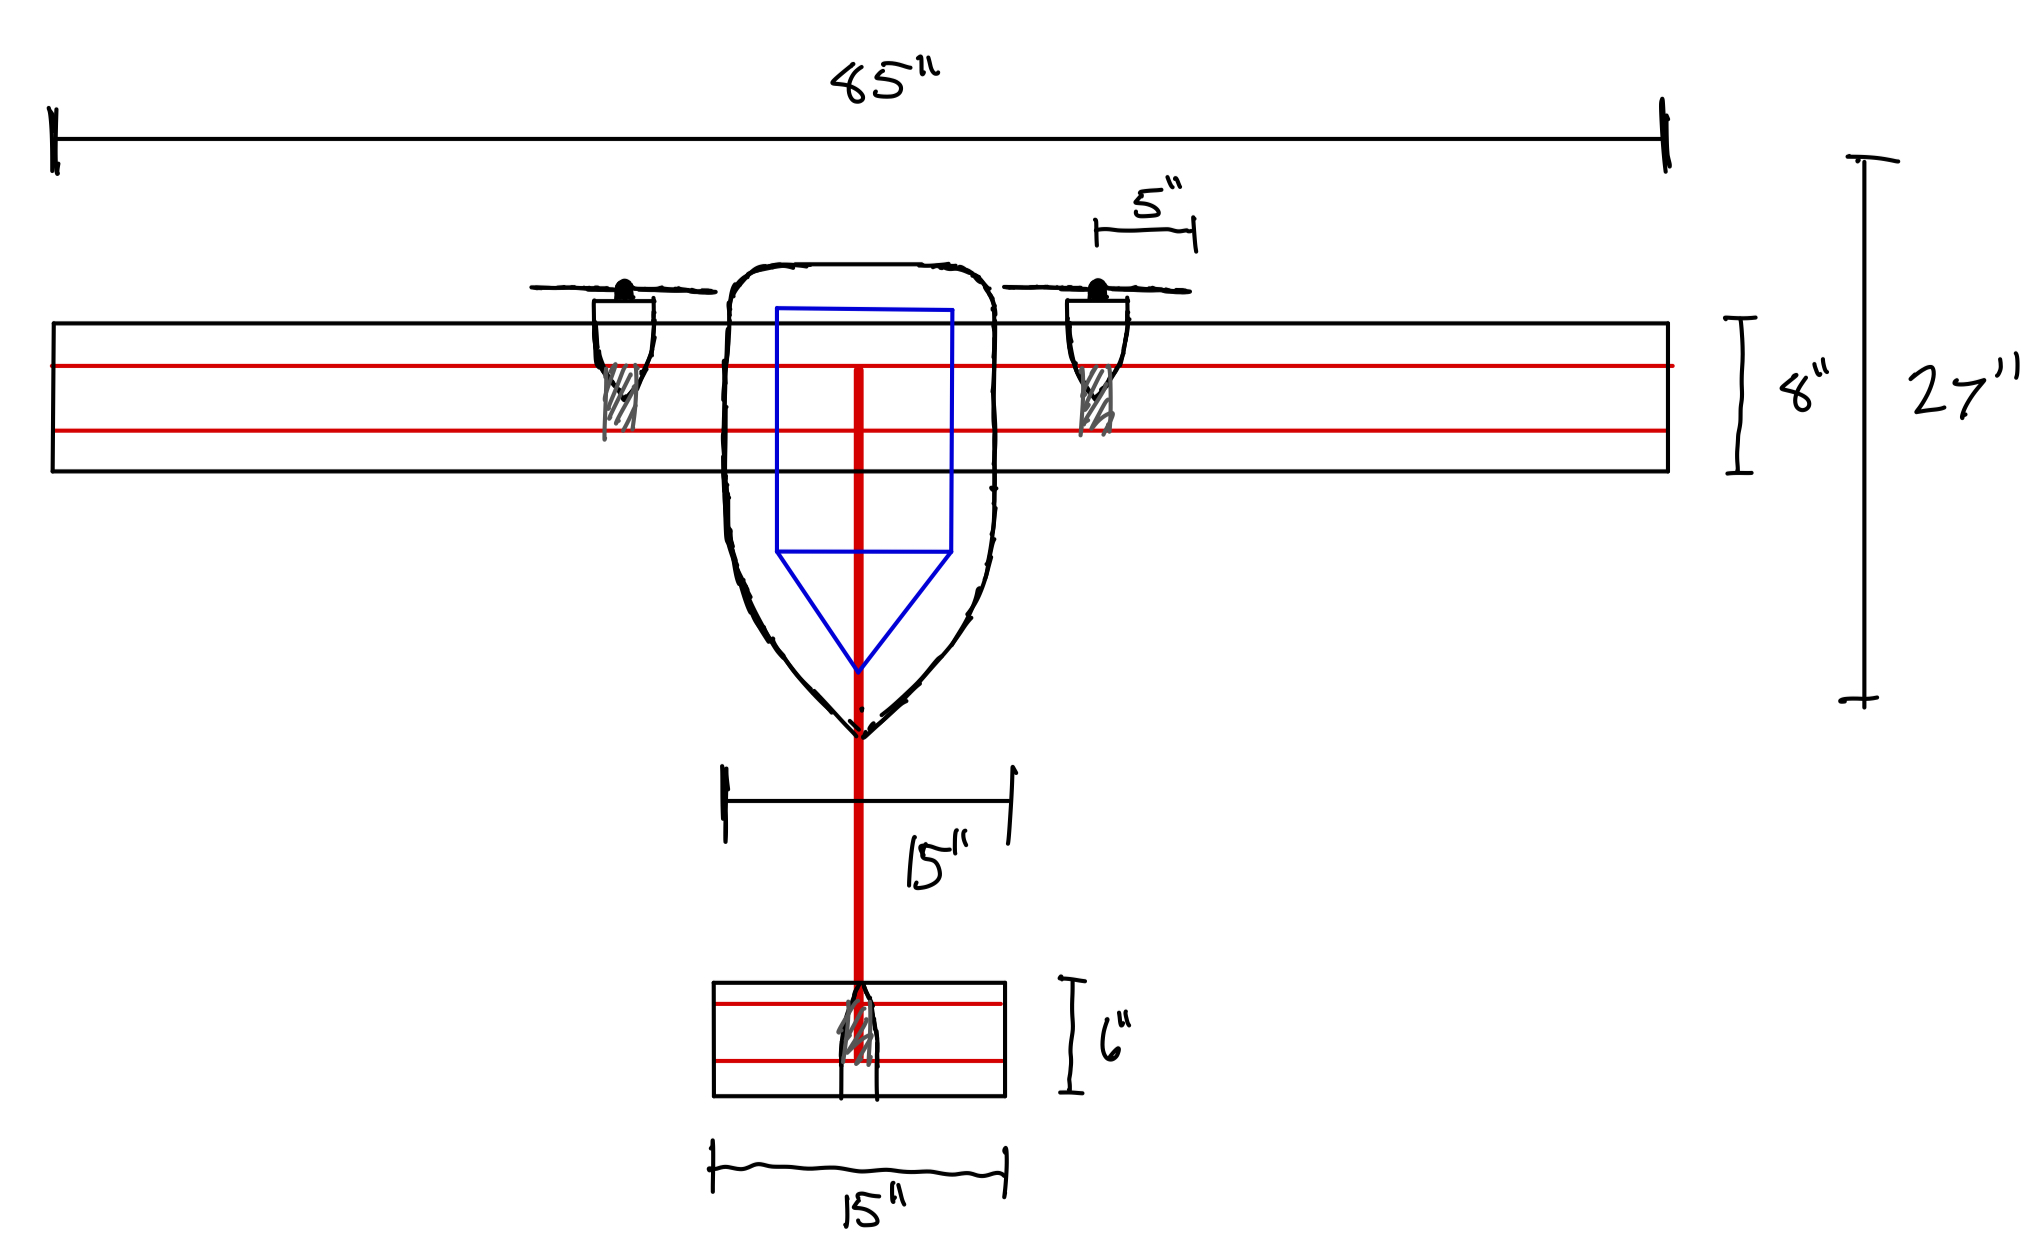
\includegraphics[width=\linewidth]{figures/Initial Design 2.jpeg}
    \end{frame}
    
    
    \begin{frame}{Initial Design III}
        \centering
        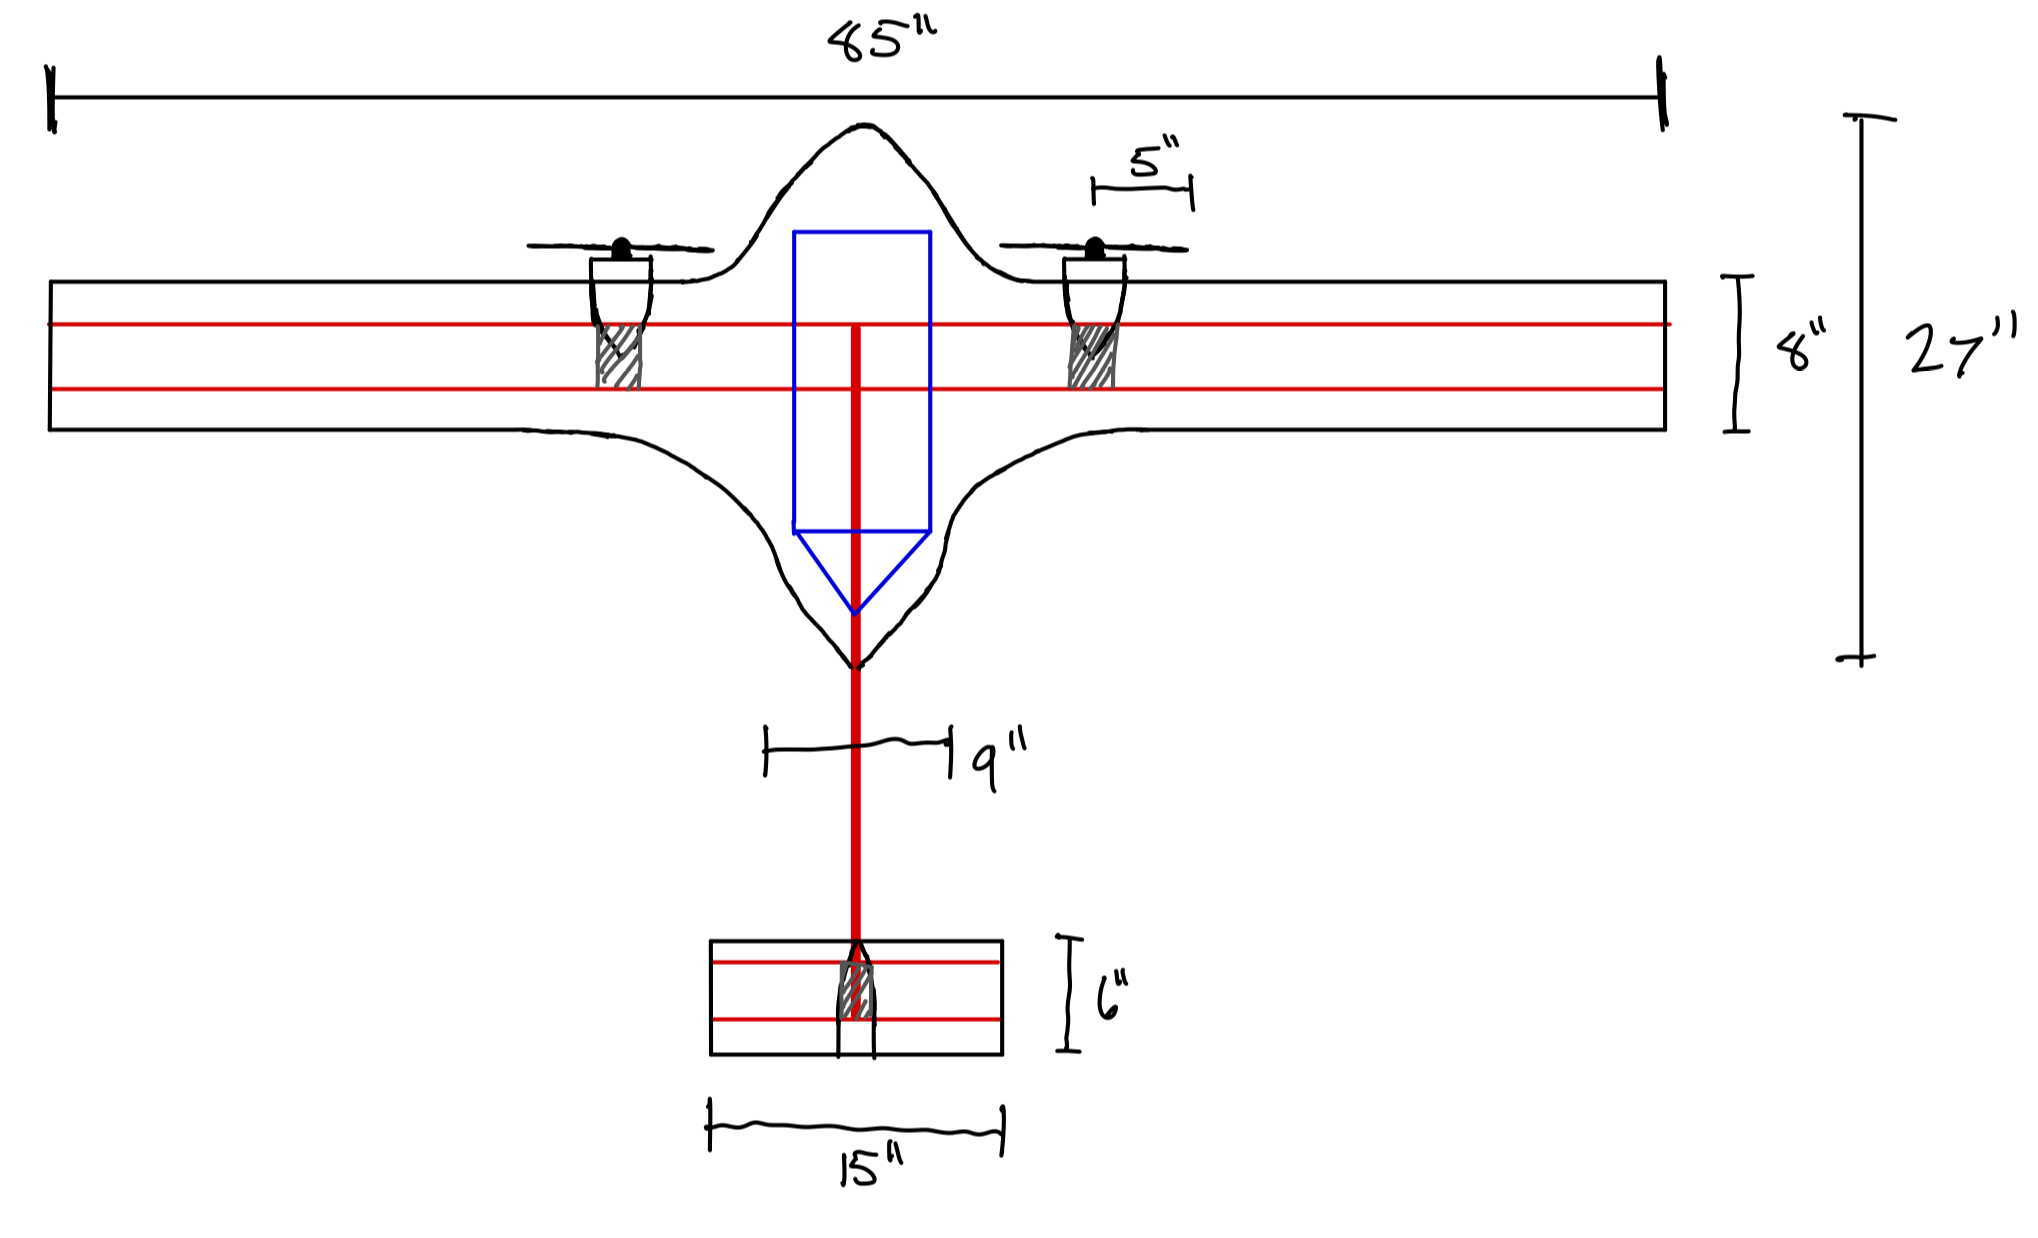
\includegraphics[width=\linewidth]{figures/Initial Design 3.jpeg}
    \end{frame}

    \begin{frame}{Initial Design}
        \centering
        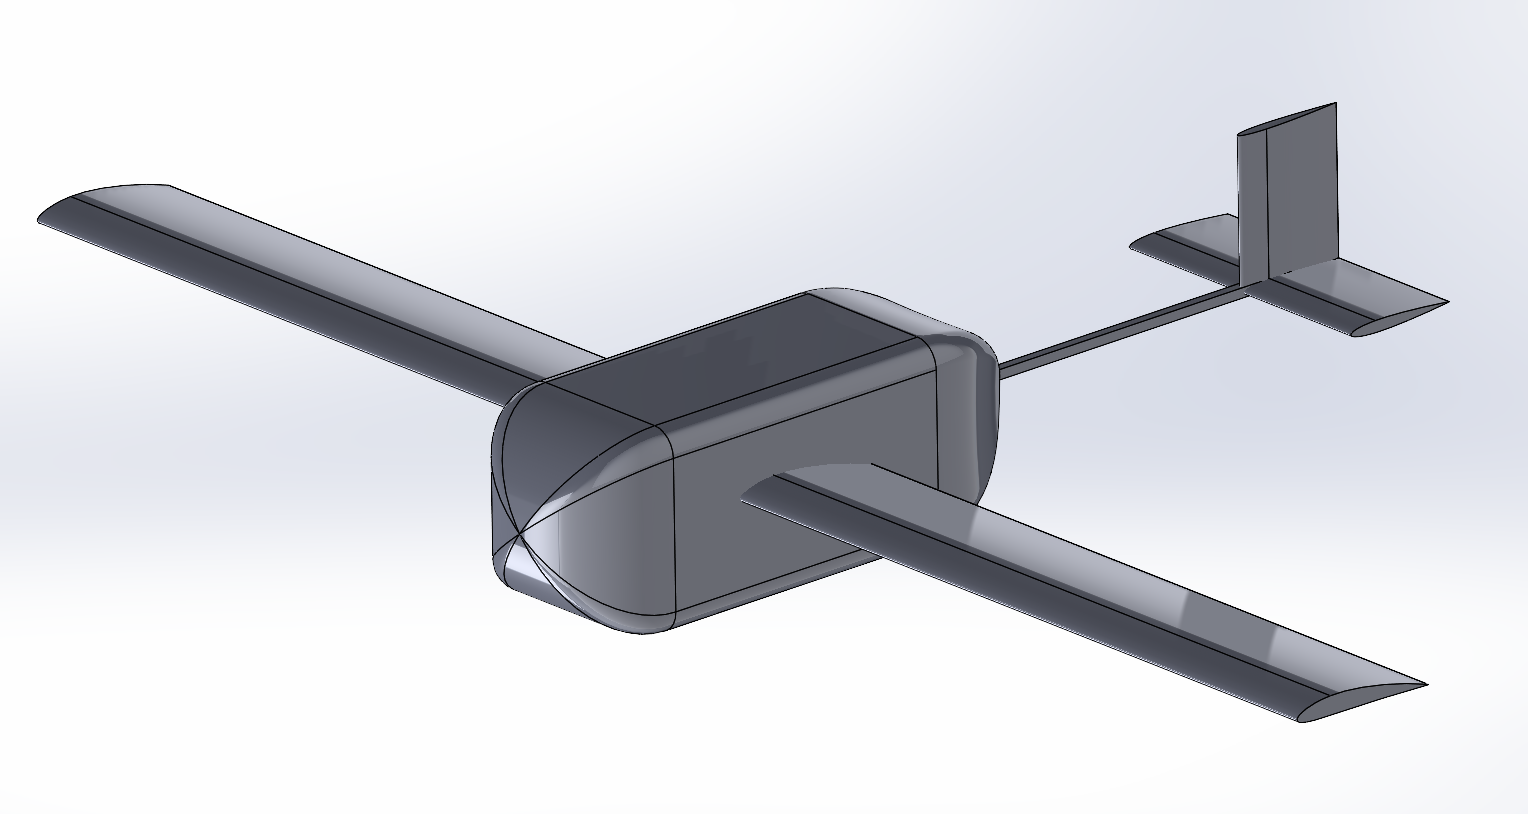
\includegraphics[width=\linewidth]{figures/isometrics over time/Assem1.0.1Iso.png}
        
    \end{frame}

    \section{Trade Studies}

    \subsection{Flight Performance}

    \subsubsection{Airfoil Selection}
    \setpresentername{Patricia Ovono}
    \setpresentertitle{Flight Performance Engineer}
    

    \begin{frame}{Primary Wing Airfoil Selection I}
        \centering
         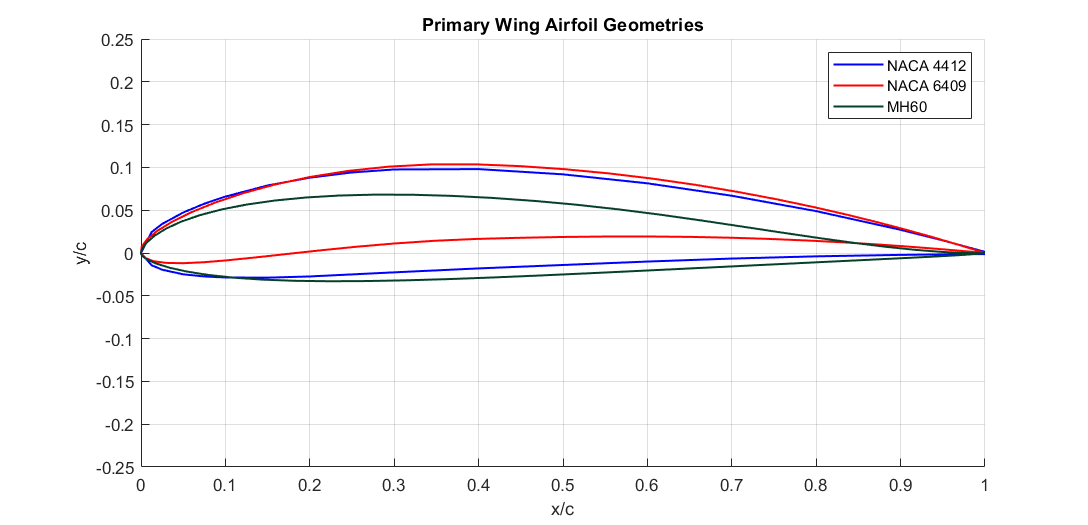
\includegraphics[width=\textwidth]{figures/Mainfoils.png}
    \end{frame}

    \begin{frame}{Primary Wing Airfoil Selection II}
        % \begin{itemize}

        % \end{itemize}
        \centering
        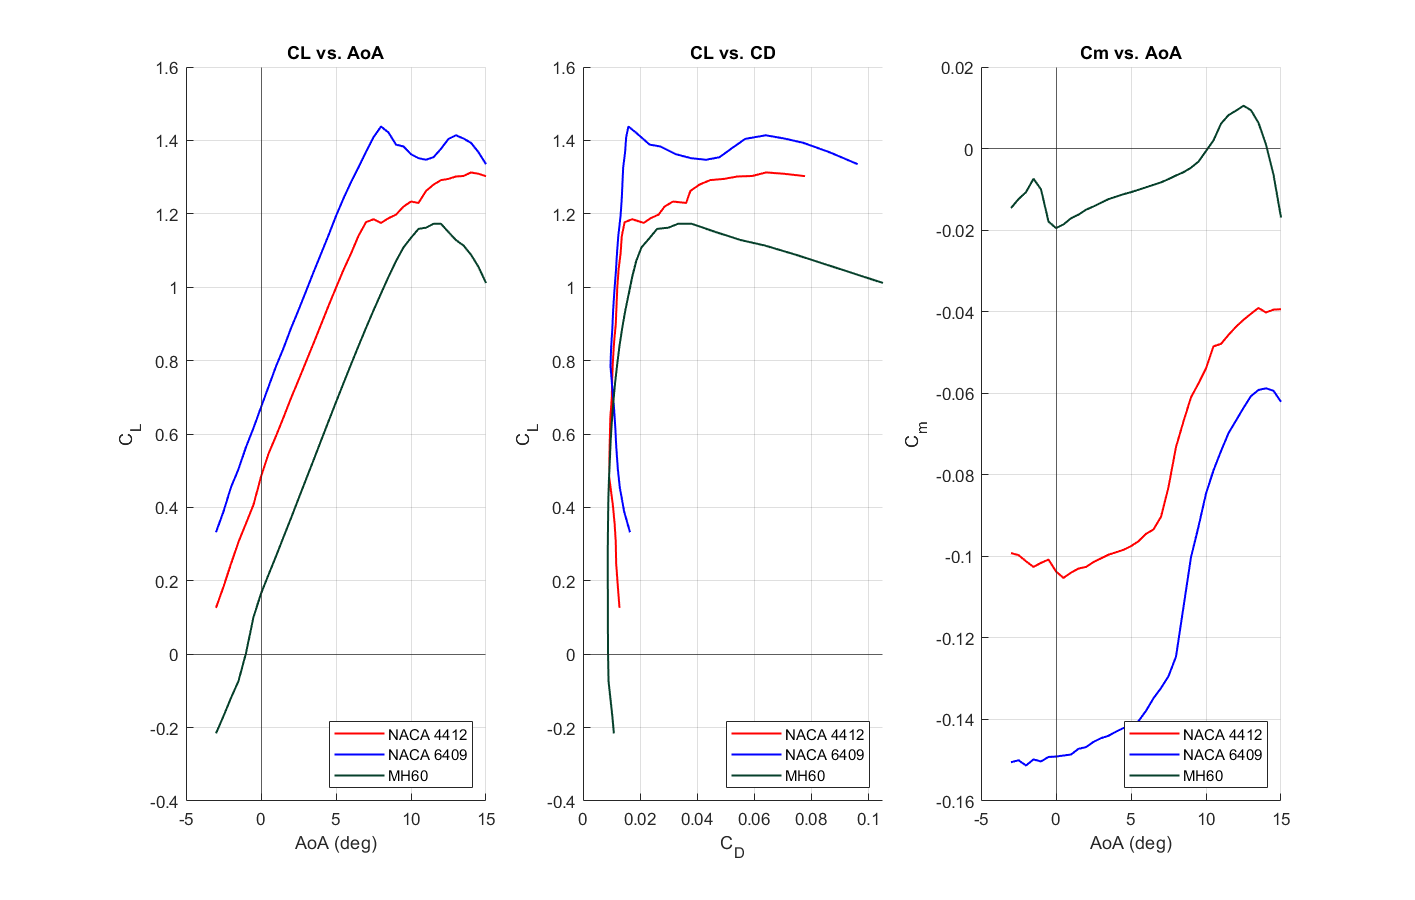
\includegraphics[width=\textwidth]{figures/primarywingplots.png}
    \end{frame}
    
    \begin{frame}{Tail Wing Airfoil Selection I}
        \centering
         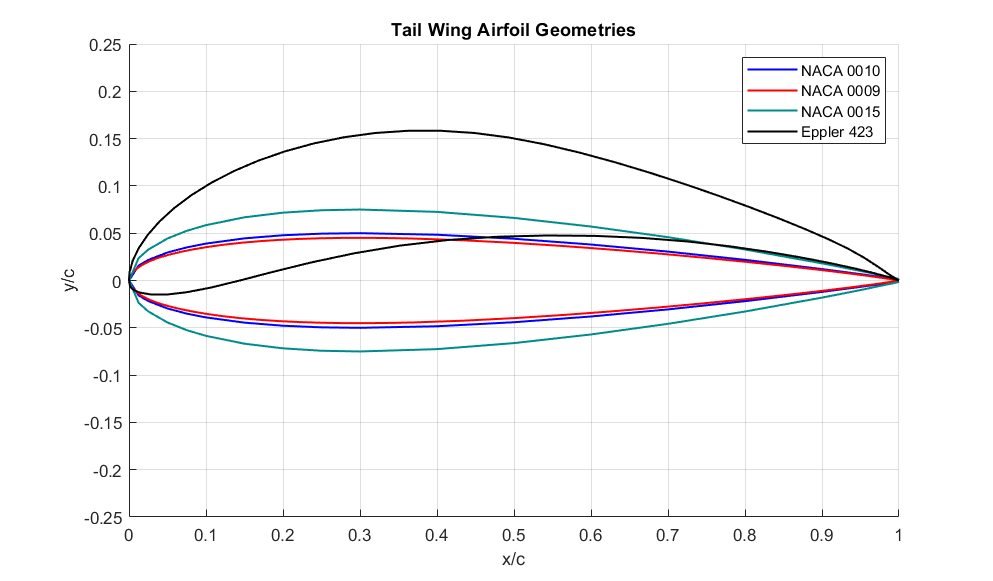
\includegraphics[width=\textwidth]{figures/tailfoils.png}
    \end{frame}
        
    % \begin{frame}{Tail Wing Airfoil Selection II}
    %     \begin{itemize}
    %         \item E423 produced too much lift for a tail stabilizer airfoil
    %         \item NACA 0009 and NACA 0010 data was largely the same but were too thin for tail spars
    %         \item Picked the NACA 0015 foil for easier manufacturing
    %     \end{itemize}
    % \end{frame}

    \begin{frame}{Initial Airfoil Selection Summary}
        % Notes
        % Initially chose NACA 4412 for wing airfoils
        % - Produces high lift at low speeds and generates large,  unstable pitching moments
        % Initially chose NACA 0010 for tail airfoils 
        % - Thickness of tail did not accommodate tail spars, opted for NACA 0015
        \begin{itemize}
            \item Initial choice:
            \begin{itemize}
                \item Primary wing: NACA 4412
                \item Tail: NACA 0015
            \end{itemize}
            % this shit comes from https://m-selig.ae.illinois.edu/ads/coord_database.html pls cite thnks bbg <3
        \end{itemize}
        \centering
        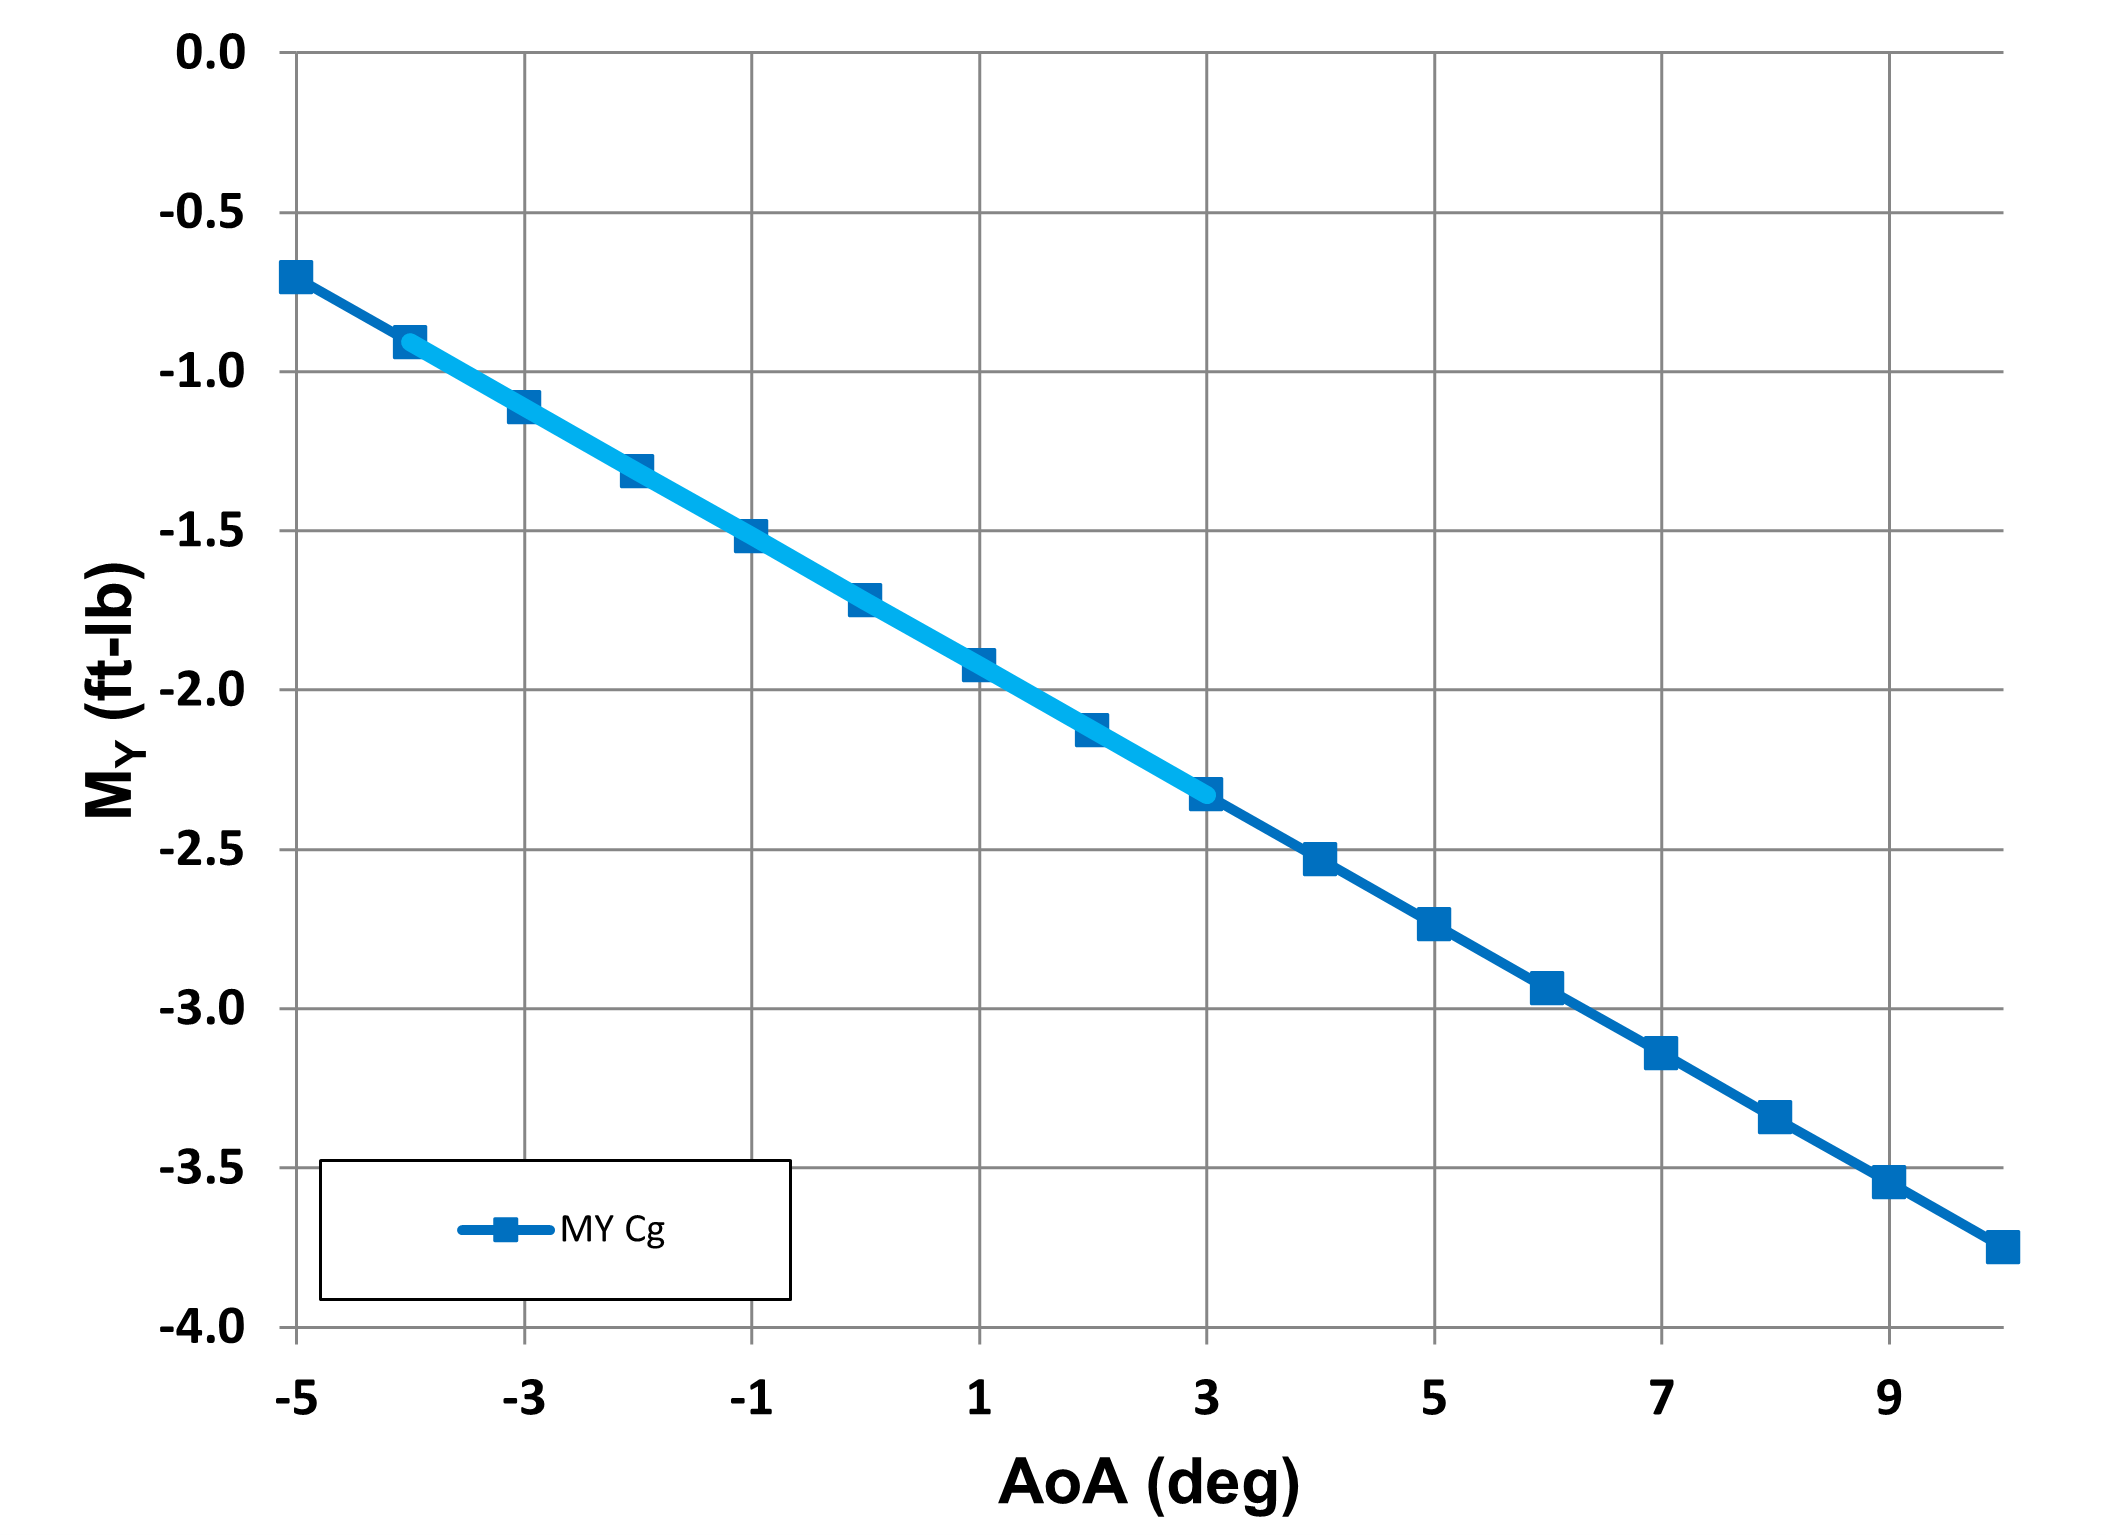
\includegraphics[width=0.75\linewidth]{figures/pitchV1.1.12.png}
    \end{frame}

    \begin{frame}{NACA 2412 vs. NACA 4412 I}
        \centering
        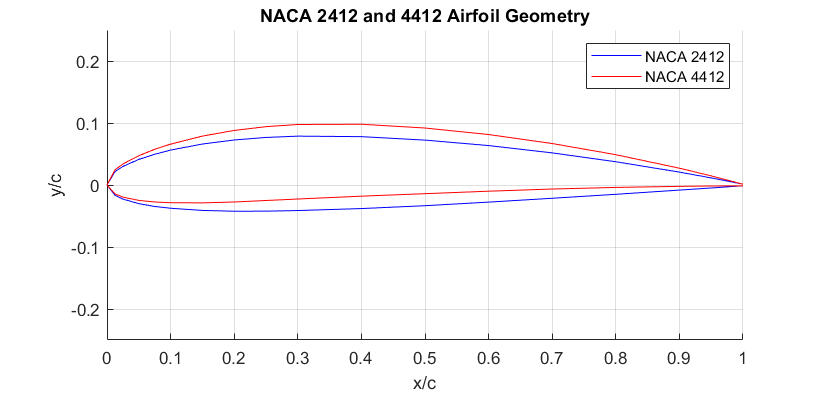
\includegraphics[width=\textwidth]{figures/newfoil.png}
    \end{frame}

    \begin{frame}{NACA 2412 vs. NACA 4412 II}
        \centering
        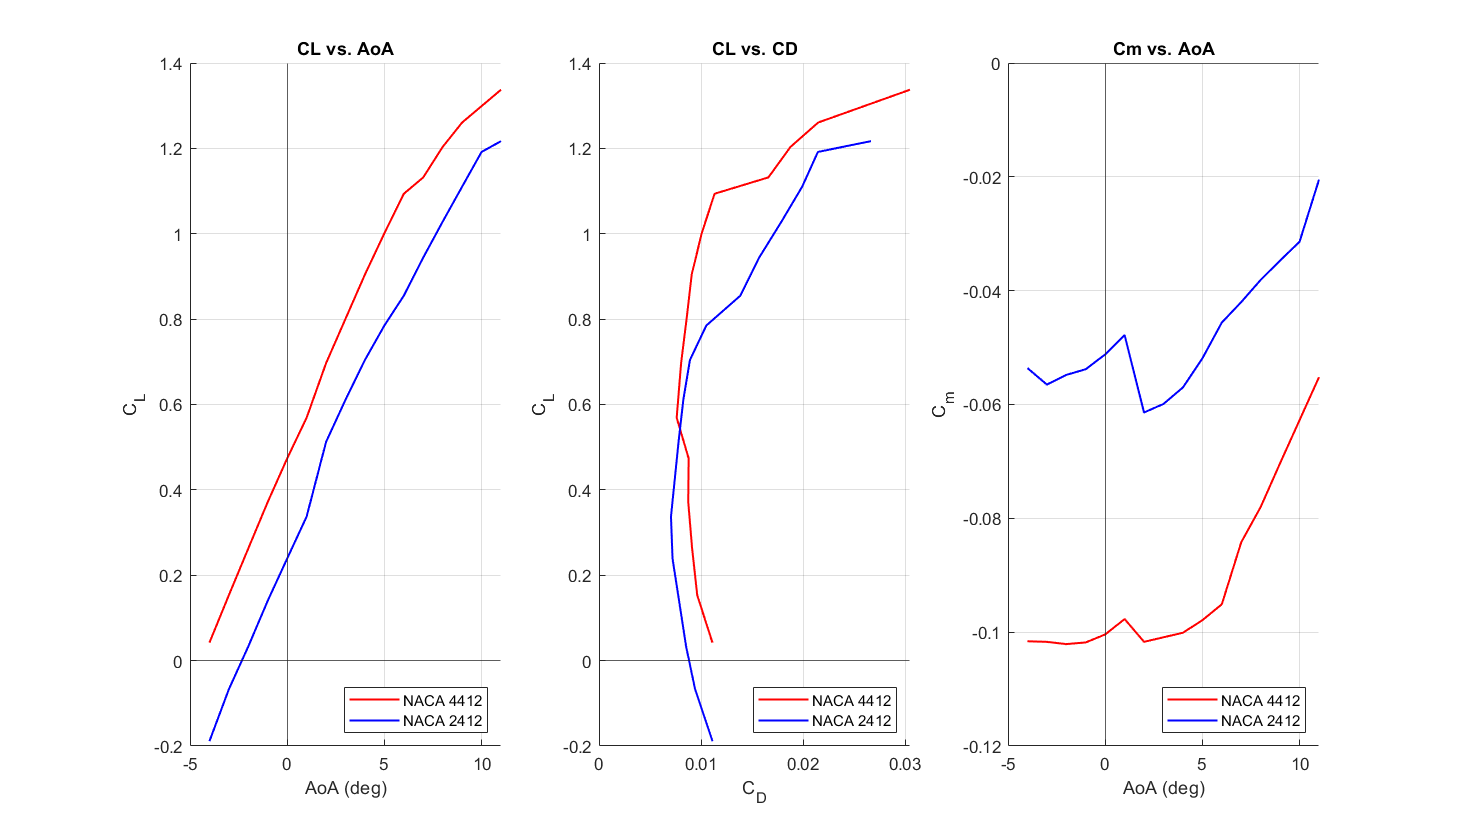
\includegraphics[width=\textwidth]{figures/newfoilplots.png}
    \end{frame}

    \subsubsection{Wing Sizing and Placement}
    % \begin{frame}{Wing Placement Configurations}
    % \begin{itemize}
    %     \item Need to analyze the influence of primary wing position on the location of aerodynamic center
    %     \item Tested range of wing positions 
    %     \begin{itemize}
    %         \item from 7" back from the nose to 10".
    %         \item 7" back moves neutral point closer to CG. 10" back moves neutral point away
    %     \end{itemize}
    % \end{itemize}
    %     % Should show the initial and a representative sample of the other wing placement tests (for the primary and tail wing, if applicable)
    %     % This would preferably be a graphic of some sort.
    % \end{frame}
    \setpresentername{Thomas Housley}
    \setpresentertitle{Lead Flight Performance Engineer}
    \begin{frame}{Wing Placement Analysis}
        % Show the results of the wing placement studies. Choose representative data points if the data is too cluttered.
    \begin{figure}
        \centering
        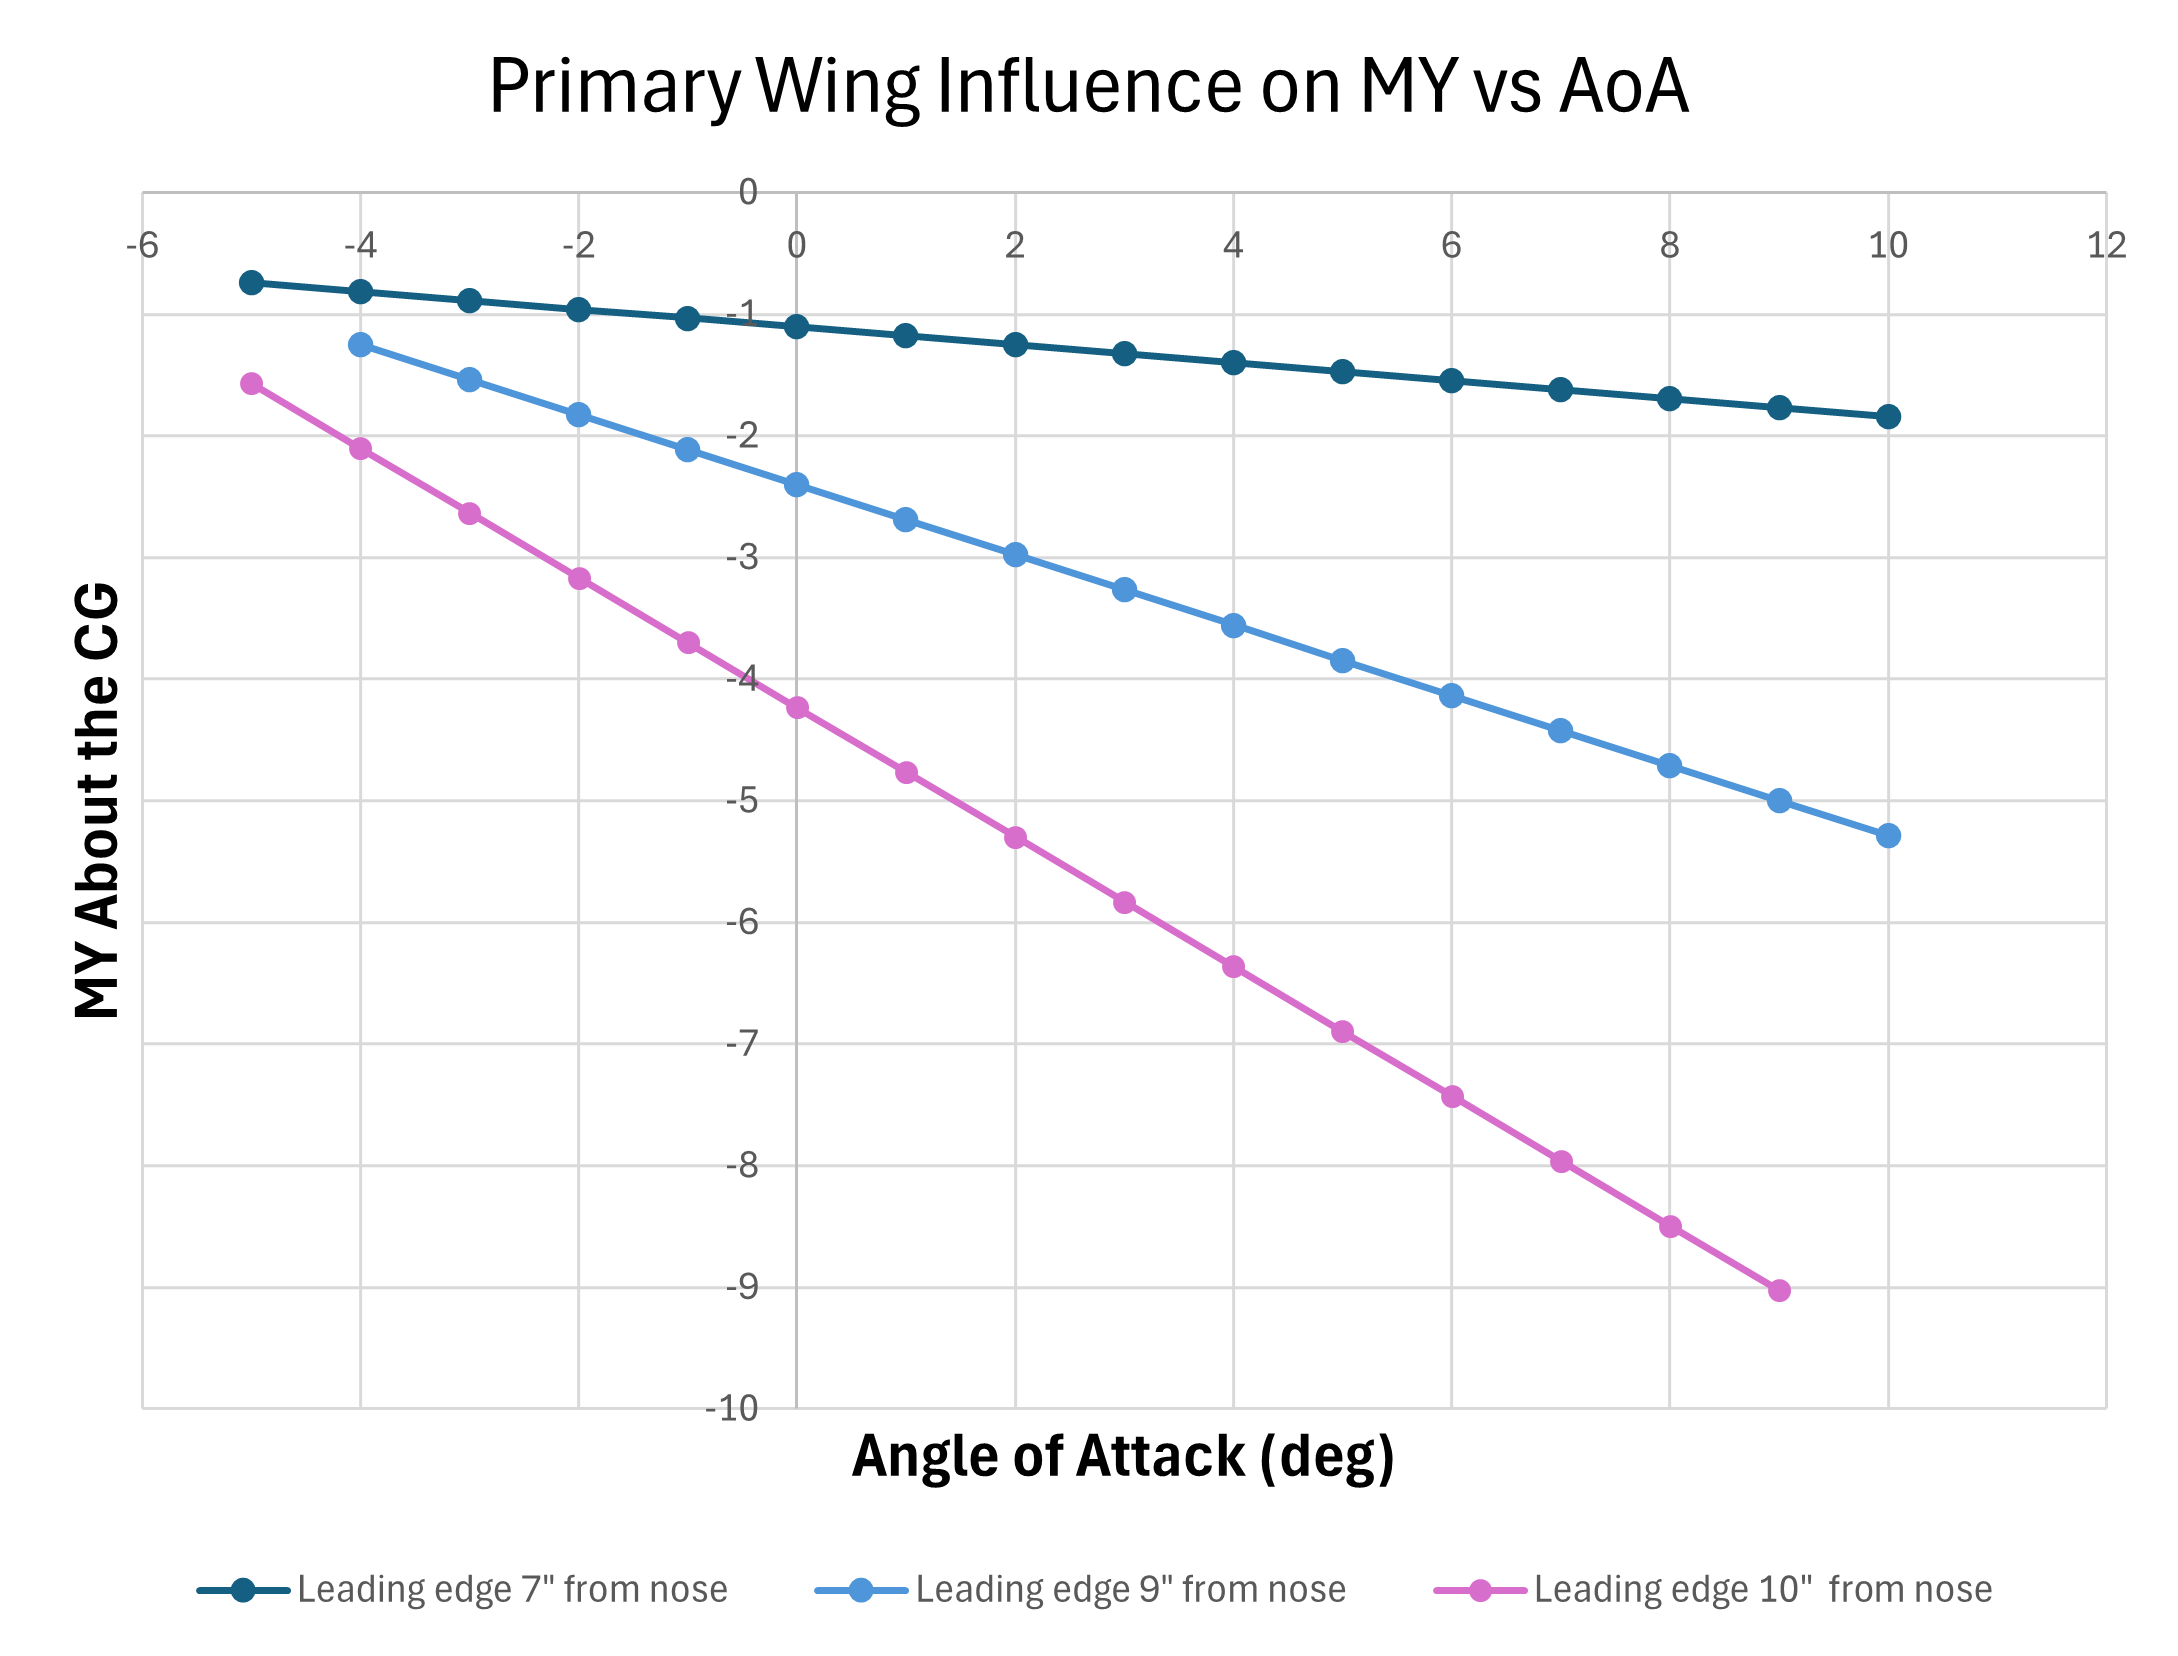
\includegraphics[width=.9\linewidth]{figures/prettygraf.png}
    \end{figure}
    \end{frame}


    
    % \begin{frame}{Wing Sizing Configurations}
    % \begin{itemize}
    %     \item Our initial chord length (8in) was too small
    %     \item Horizontal tail span (12in) was too small
    %     \item Tested range of chord lengths and tail spans for desired pitch dynamics 
    %         \item Needed to find the relationship between primary wing and tail platform area against pitch moment about the center of gravity,


    % \end{itemize}
    %     % Should show the initial and a representative sample of the other wing sizes tests (for the primary and tail wing, if applicable)
    %     % This would preferably be a graphic of some sort.
    % \end{frame}

    \begin{frame}{Wing Sizing Analysis}
    % \begin{itemize}
    %     \item Increasing tail platform raises $M_y$ at AoA = 0
    %     \item Increasing chord shifts curve down
    % \end{itemize}
        \centering
        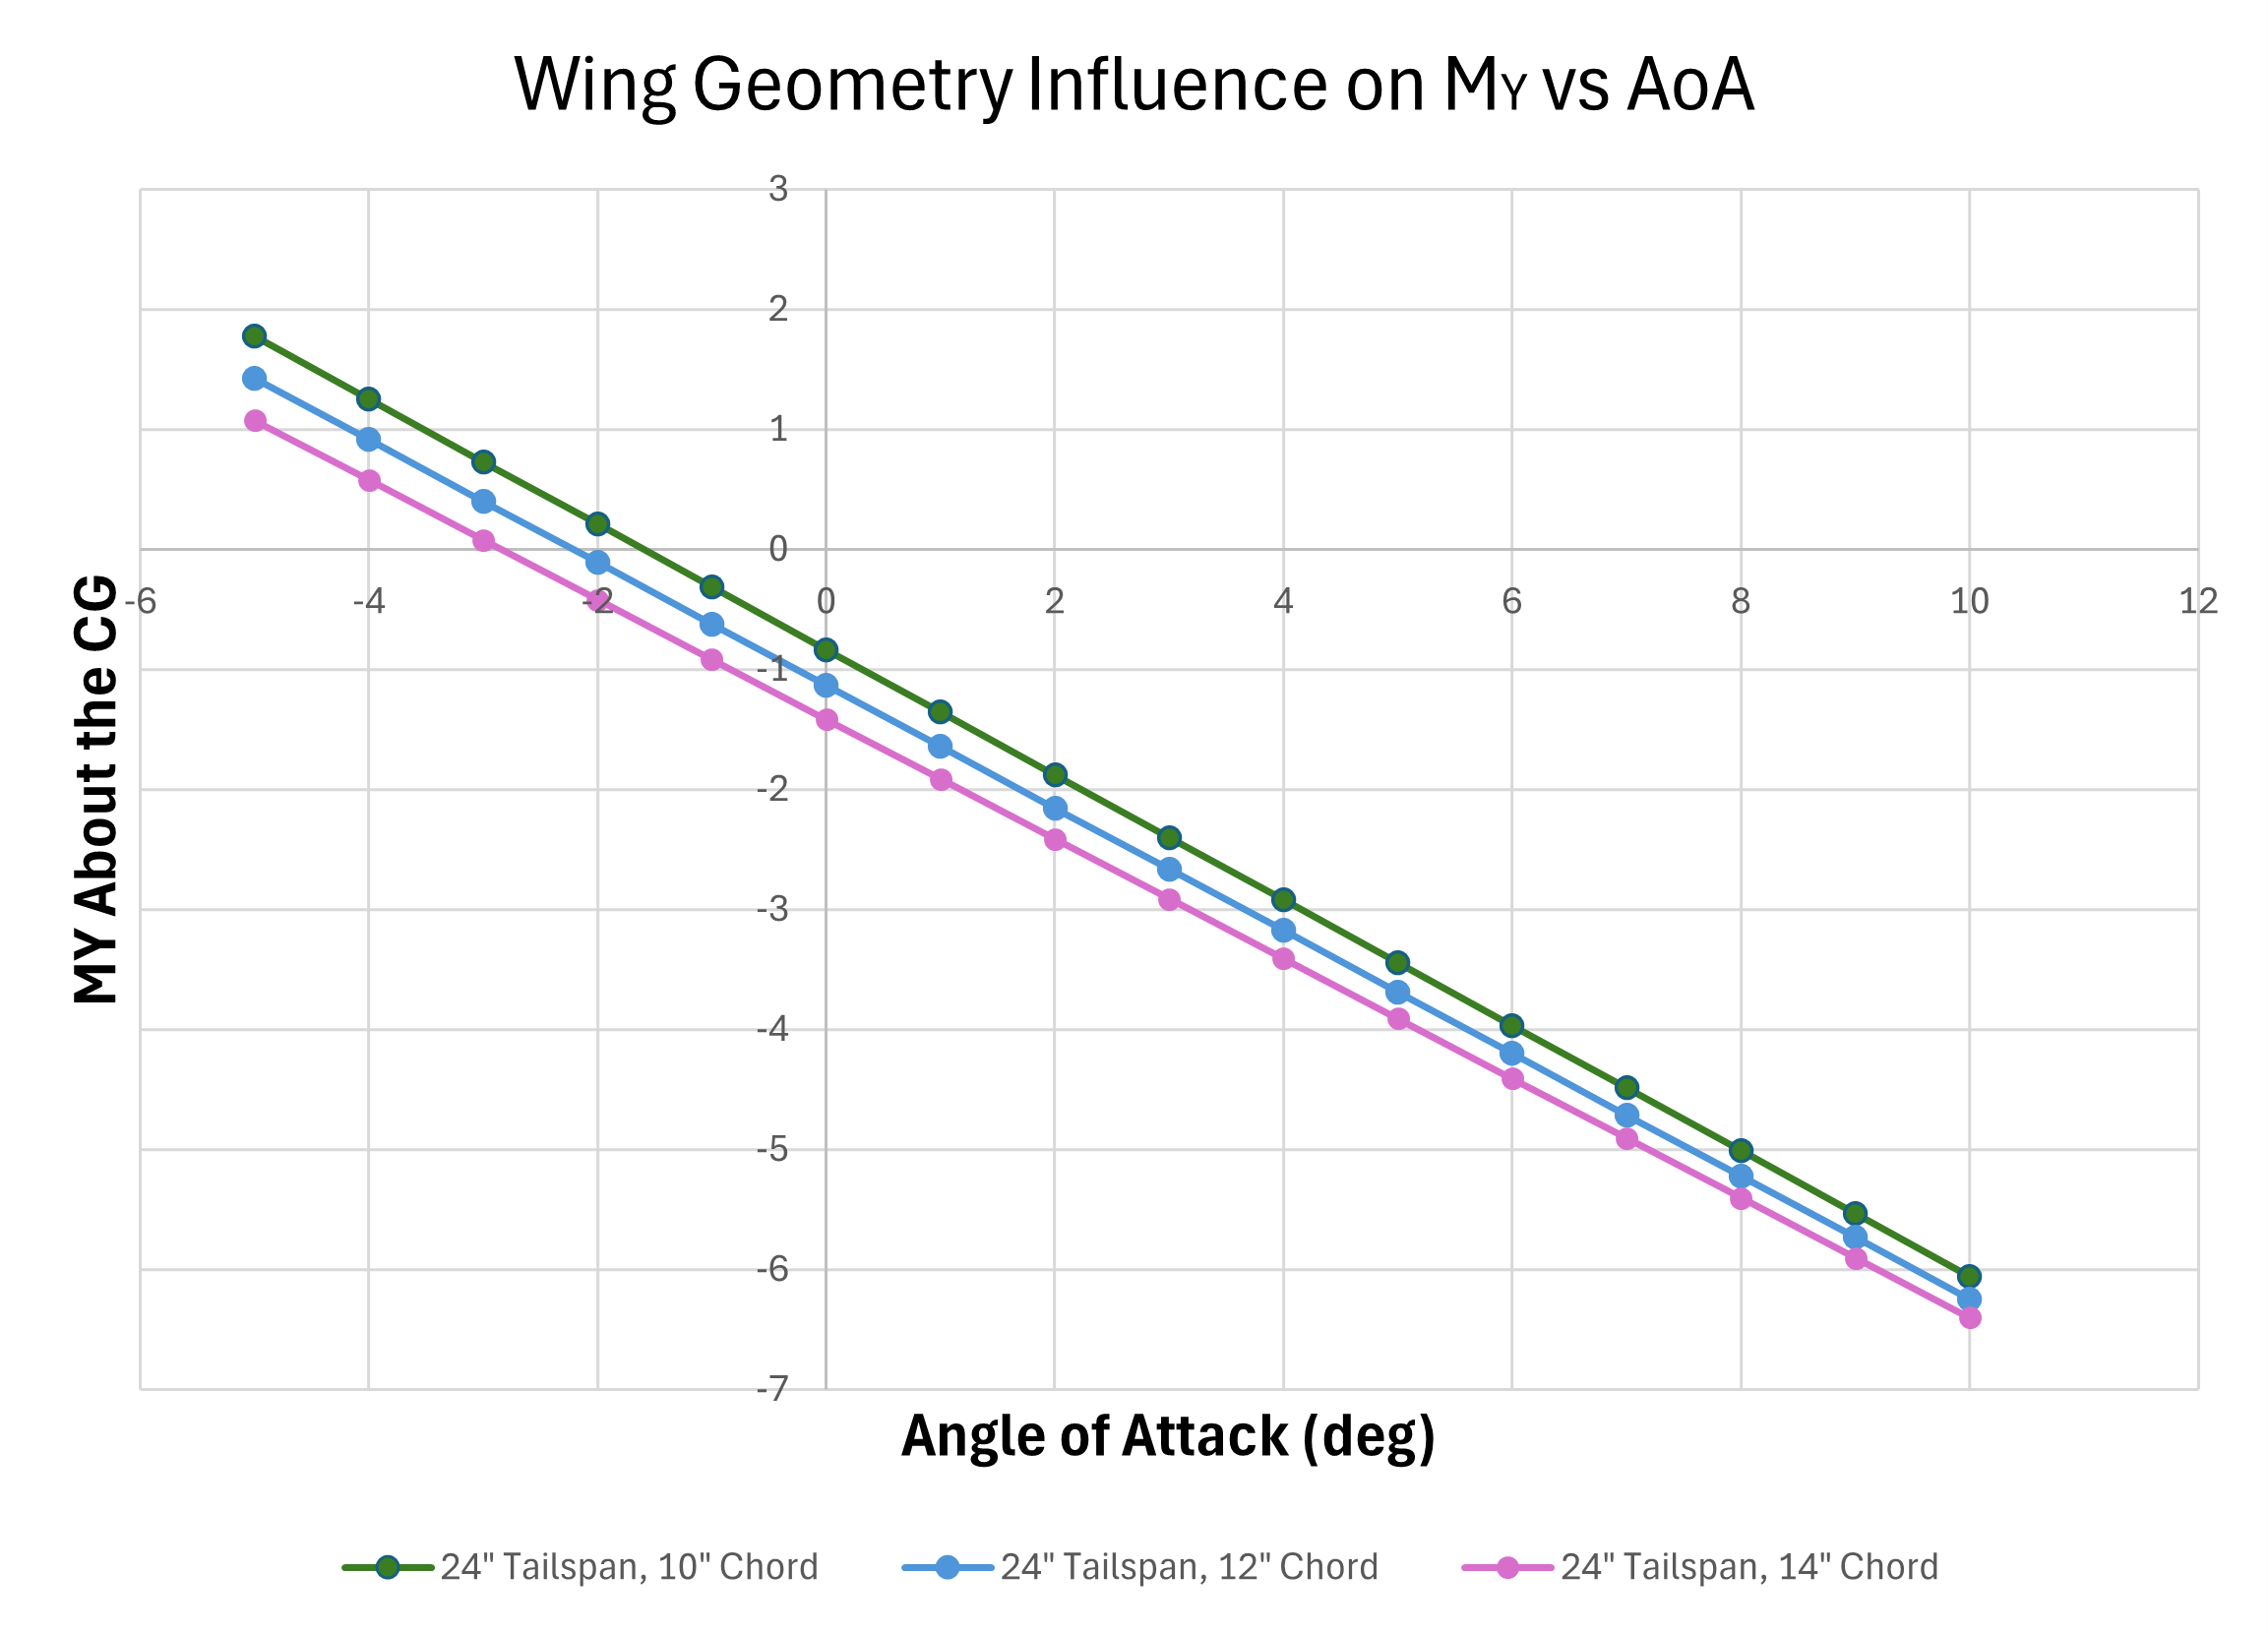
\includegraphics[width=.9\linewidth]{figures/MyVSAoa.png}
        % Show the results of the wing sizing studies. Choose representative data points if the data is too cluttered.
    \end{frame}

    \subsubsection{Fuselage Design}

    \setpresentername{Lucas Tavares Vasconcellos}
    \setpresentertitle{Structural Engineer}

\begin{frame}{Fuselage Designs}
    \begin{columns}[T]
            \begin{column}{0.5\textwidth}
                \centering
                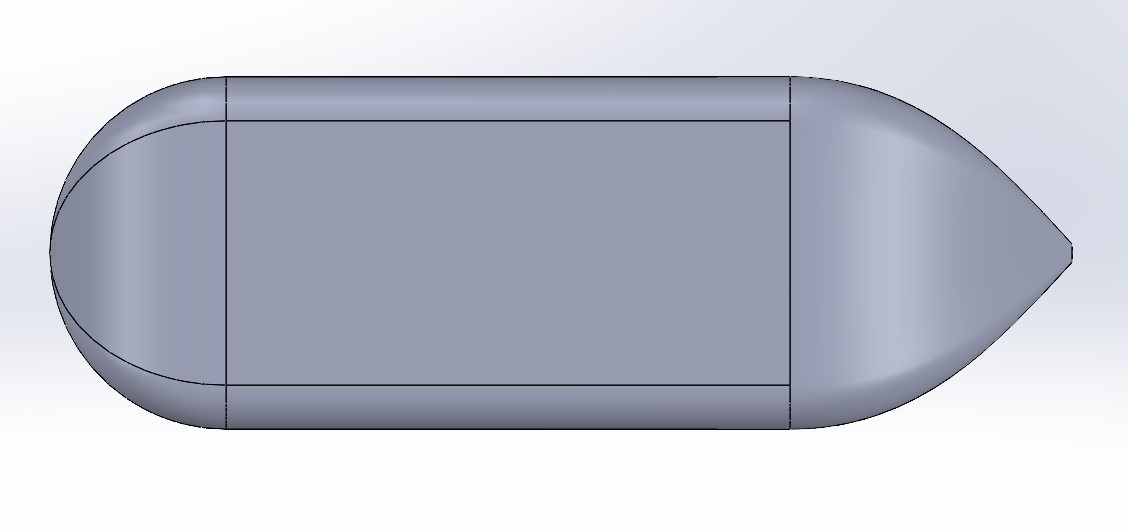
\includegraphics[width=\textwidth]{figures/fuselage/Fuselage1.0.0.jpg}
                \vspace{0.5em} % Space between image and caption
                \text{Initial Design Model}
            \end{column}
    
            \begin{column}{0.5\textwidth}
                \centering
                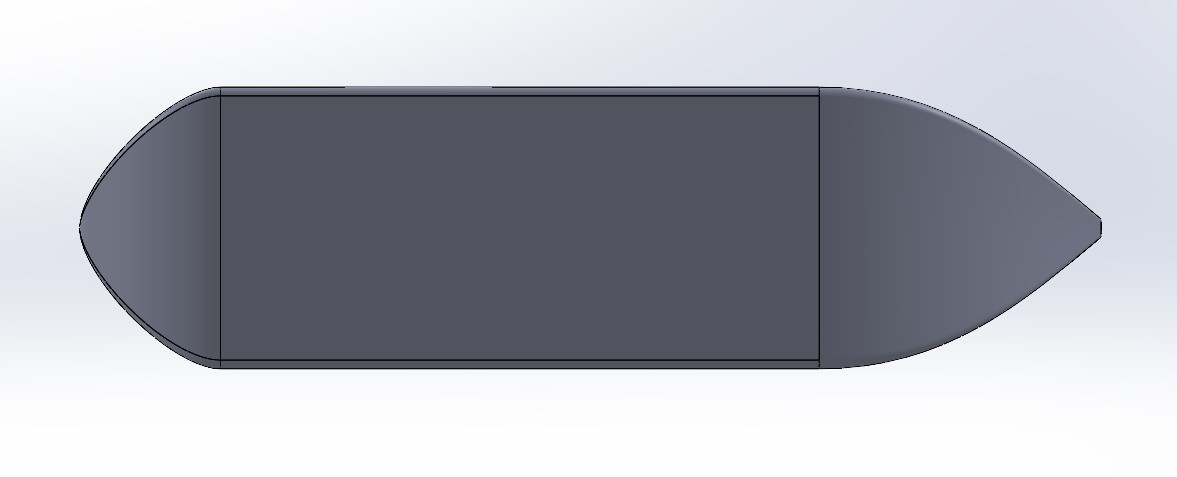
\includegraphics[width=\textwidth]{figures/fuselage/Fuselage1.2.1.jpg}
                \vspace{0.5em} % Space between image and caption
                \text{Model A}
            \end{column}
        \end{columns}
    
        \vspace{1em}
    
        \begin{columns}[T]
            \begin{column}{0.5\textwidth}
                \centering
                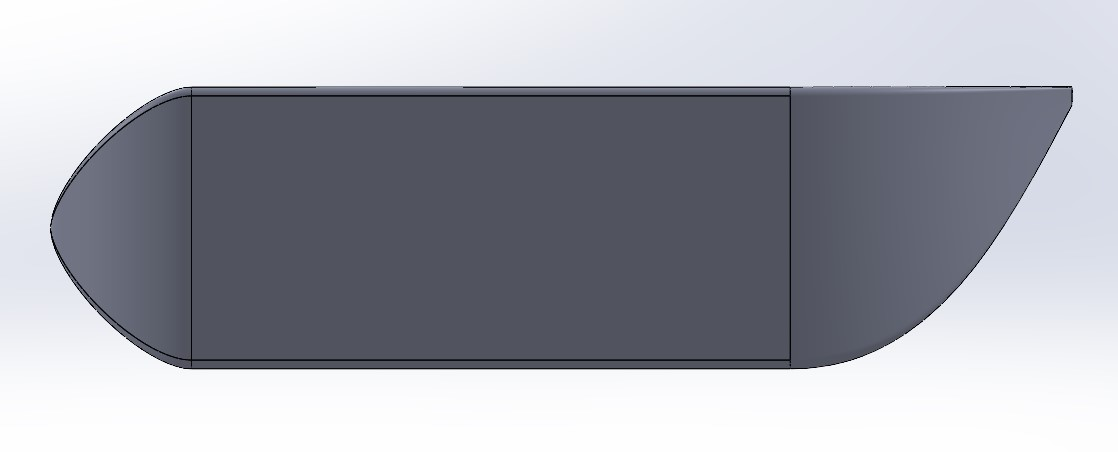
\includegraphics[width=\textwidth]{figures/fuselage/Fuselage1.2.2.jpg}
                \vspace{0.5em} % Space between image and caption
                \text{Model B}
            \end{column}
    
            \begin{column}{0.5\textwidth}
                \centering
                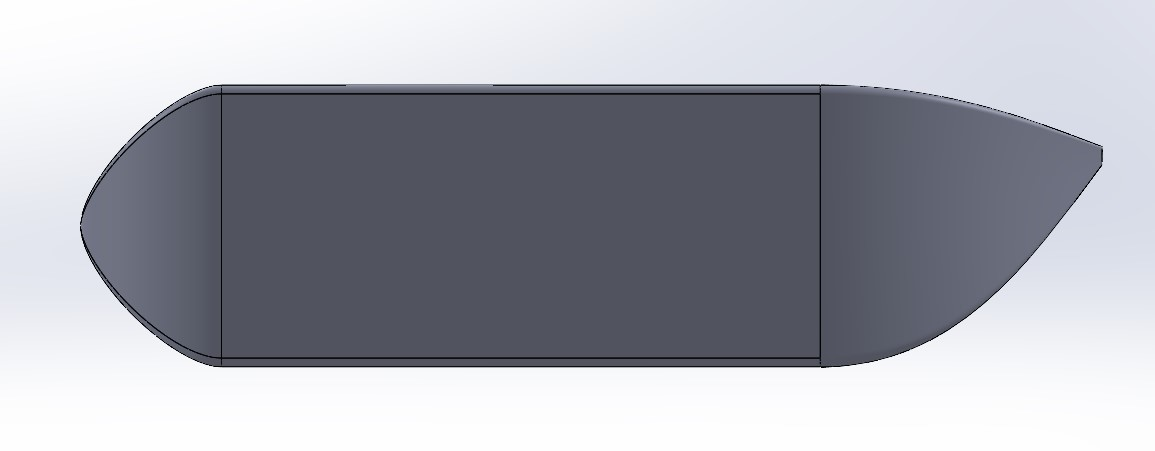
\includegraphics[width=\textwidth]{figures/fuselage/Fuselage1.2.3.jpg}
                \vspace{0.5em} % Space between image and caption
                \text{Model C}
            \end{column}
        \end{columns}
\end{frame}
    
    \subsection{Propulsion}

    \setpresentername{Lucas Tavares Vasconcellos}
    \setpresentertitle{Structural Engineer}

    \begin{frame}{Propulsion Analysis I}
        \centering
        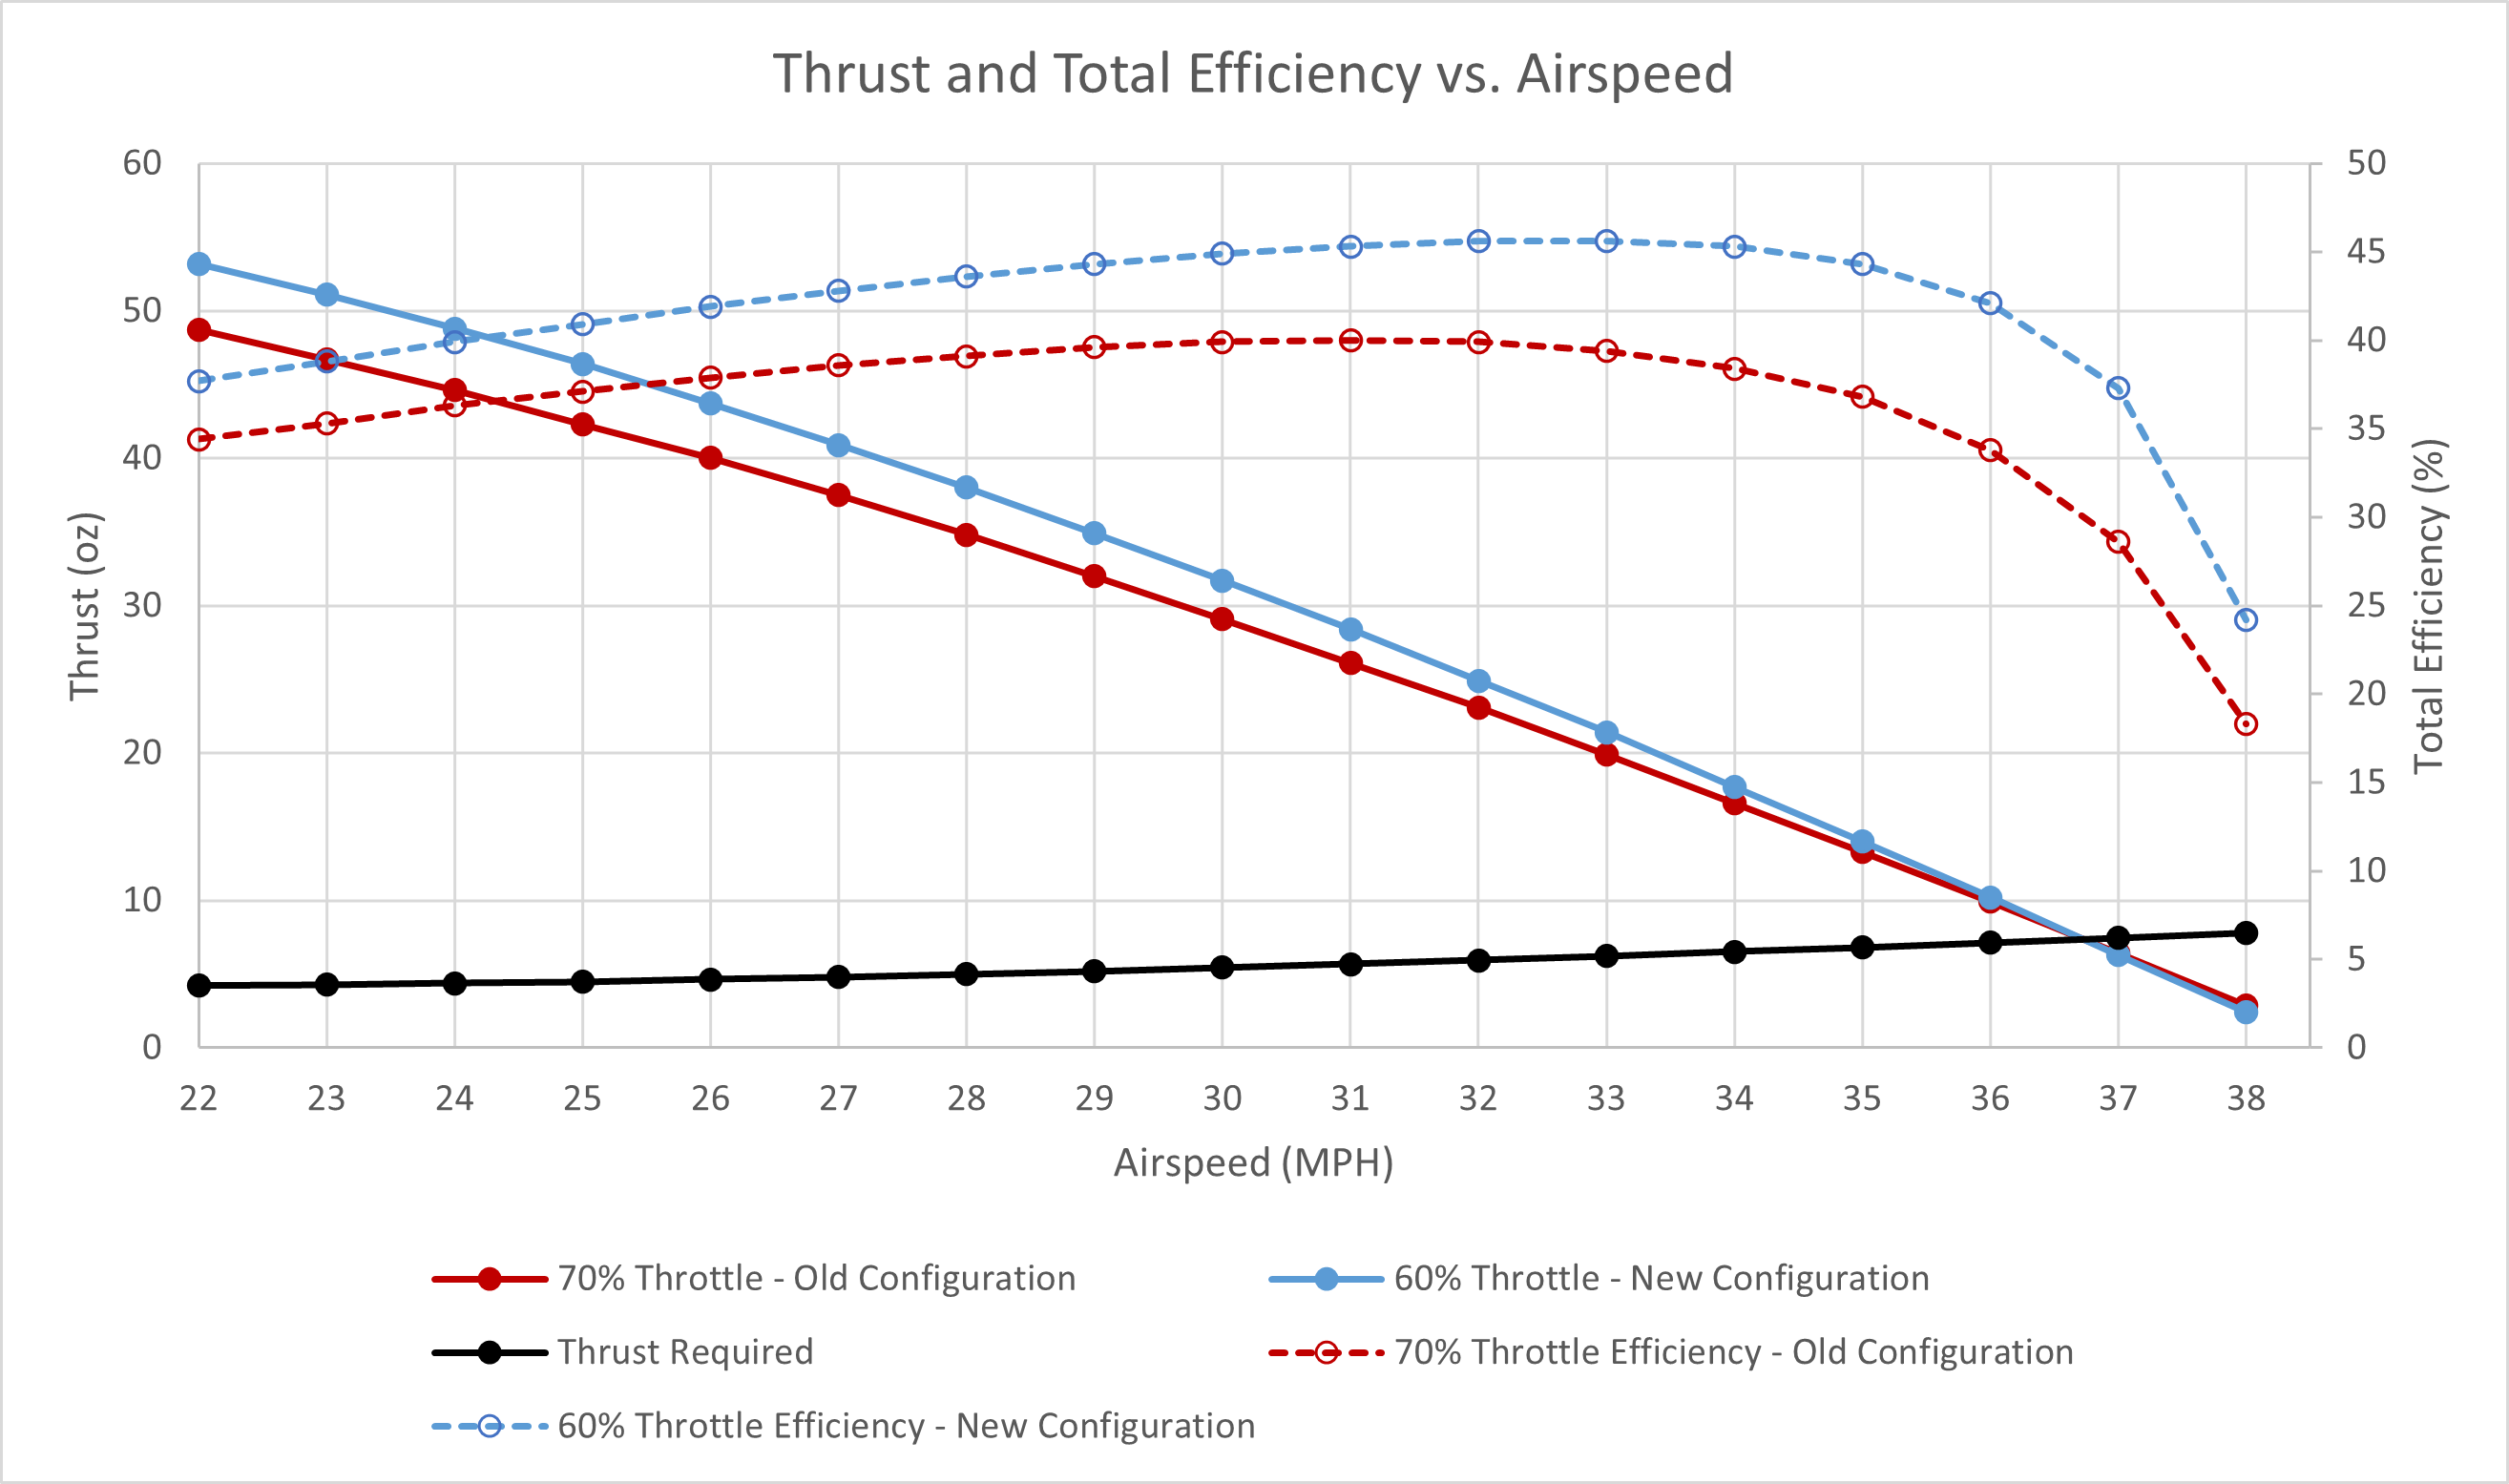
\includegraphics[width=1\linewidth]{figures/thrust_eff_vs_airspeed_comparisson.png}
    \end{frame}

    % \begin{frame}{Propulsion Analysis II}
    %     \centering
    %     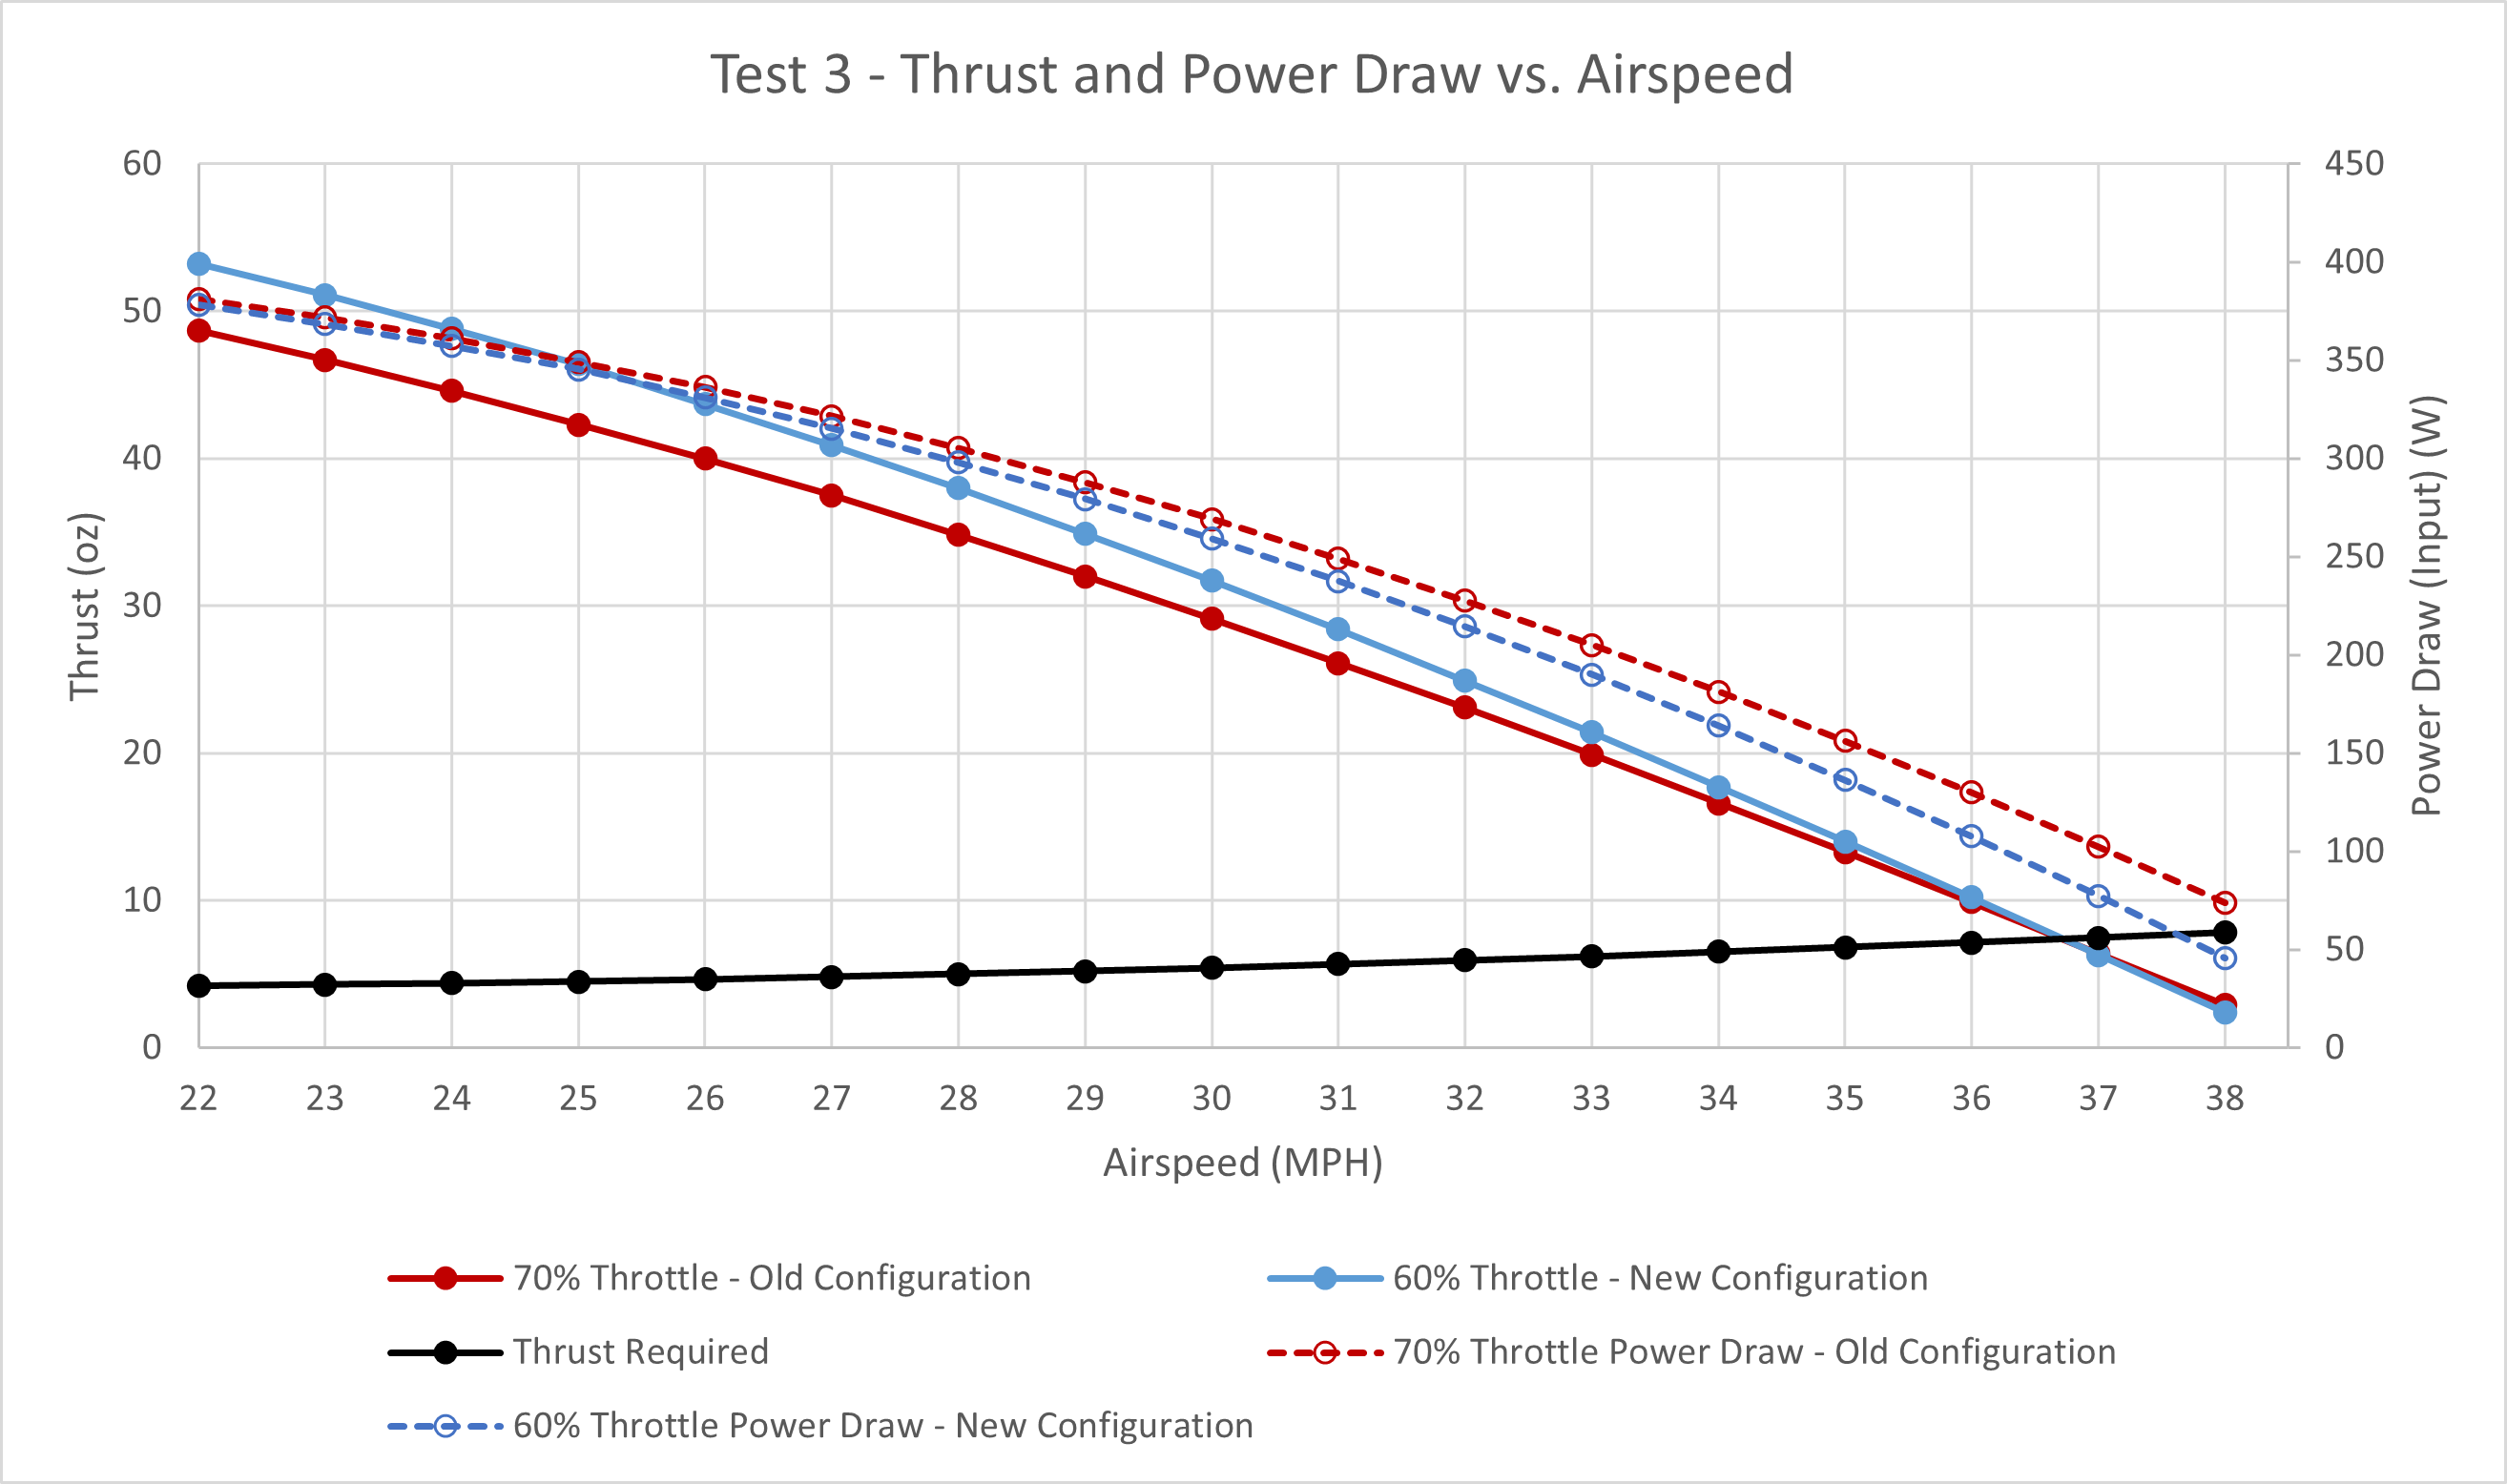
\includegraphics[width=1\linewidth]{figures/thrust_powerDraw_vs_airspeed_comparrison.png}
    % \end{frame}

    \begin{frame}{Current Propulsion System I}
        \begin{itemize}
            \item Motor: E-Flite Power 32 (770 Kv)
            \item Propeller: APC 13x6.5E
            \item Battery: Thunder Power 5S 5000 mAh
            \item Flight time at cruise speed: 40min 24s
        \end{itemize}

        \begin{figure}[htbp]
            \centering
            \begin{subfigure}{0.32\textwidth}
                \centering
                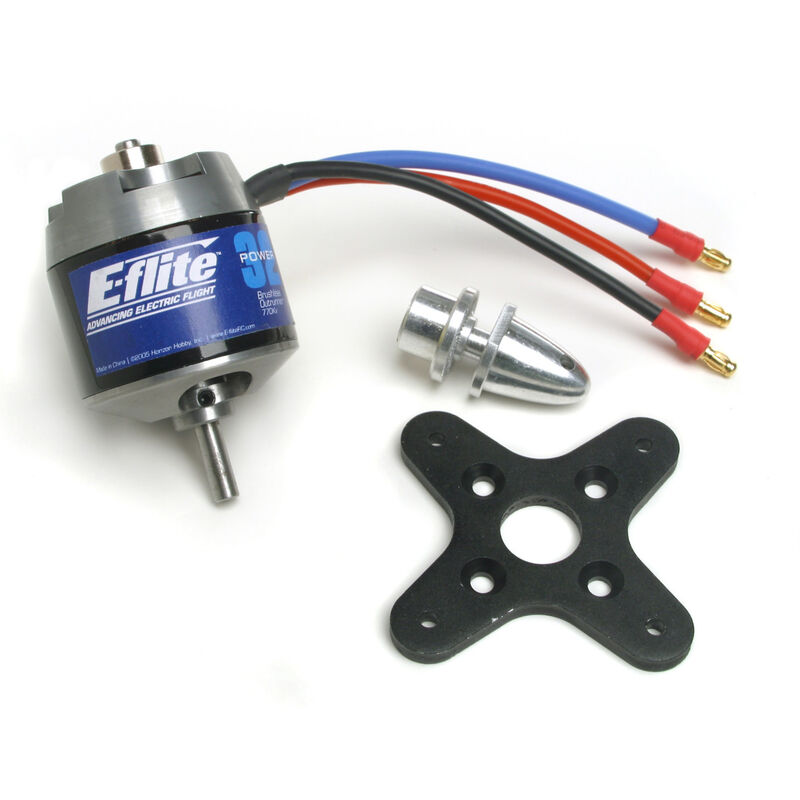
\includegraphics[width=\textwidth]{figures/eflite_motor.jpg}
            \end{subfigure}
            \hfill
            \begin{subfigure}{0.32\textwidth}
                \centering
                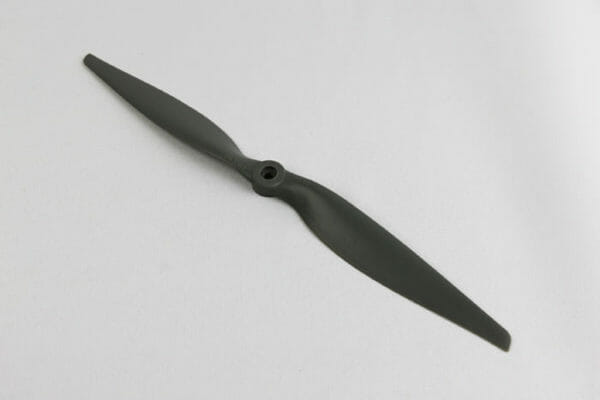
\includegraphics[width=\textwidth]{figures/apc_prop.jpg}
            \end{subfigure}
            \hfill
            \begin{subfigure}{0.32\textwidth}
                \centering
                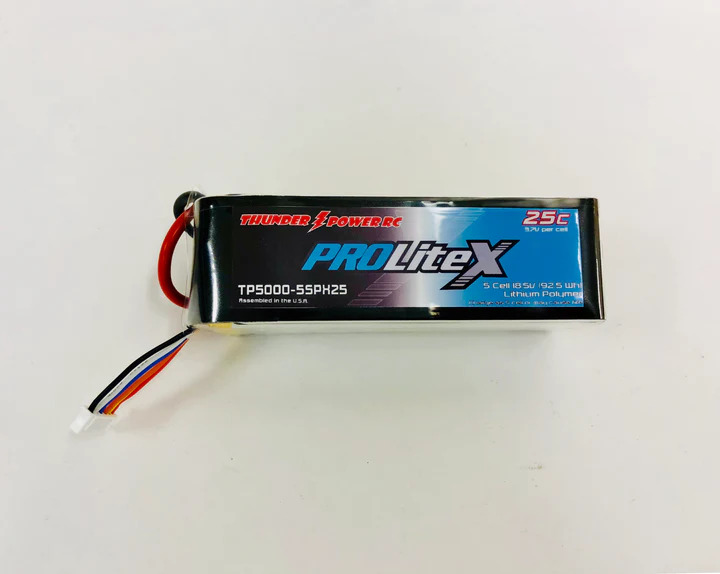
\includegraphics[width=\textwidth]{figures/tp_battery.jpg}
            \end{subfigure}
        \end{figure}
    \end{frame}

    \begin{frame}{Current Propulsion System II}
        \begin{figure}[htpb]
            \centering
            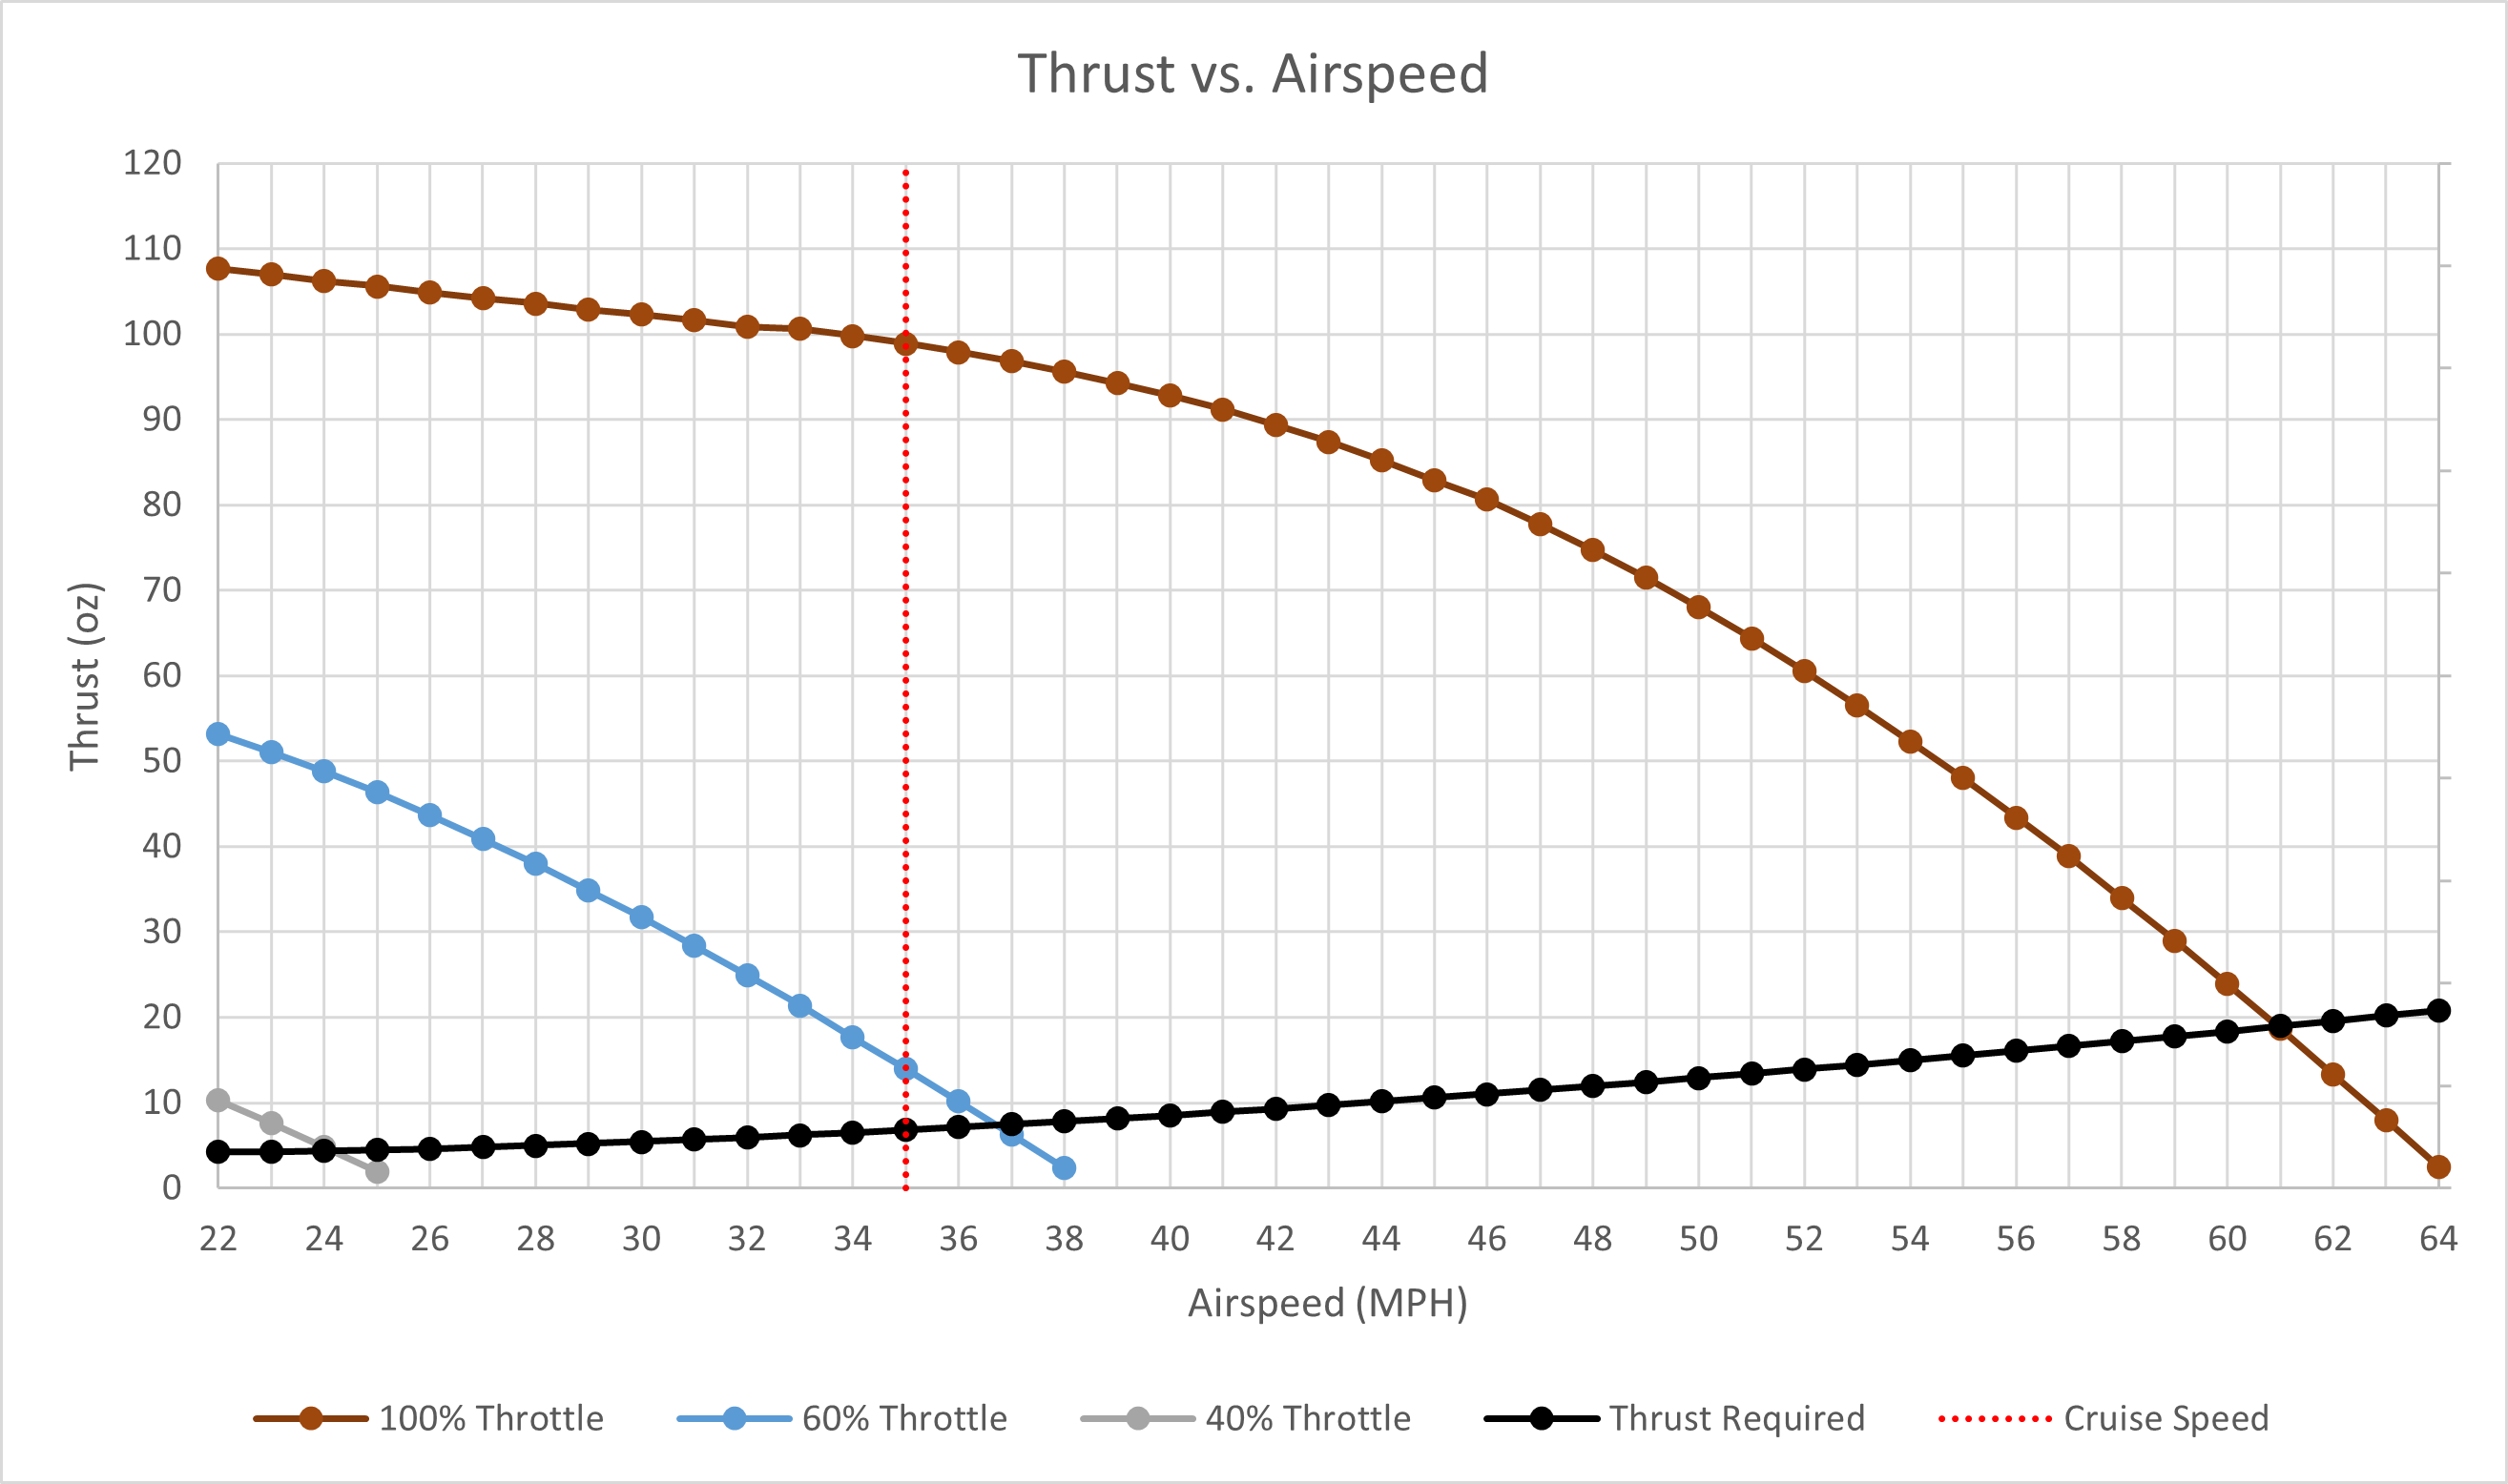
\includegraphics[width=1\linewidth]{figures/thrust_vs_airspeed.png}
        \end{figure}
    \end{frame}

    \begin{frame}{Current Propulsion System III}
        \centering
        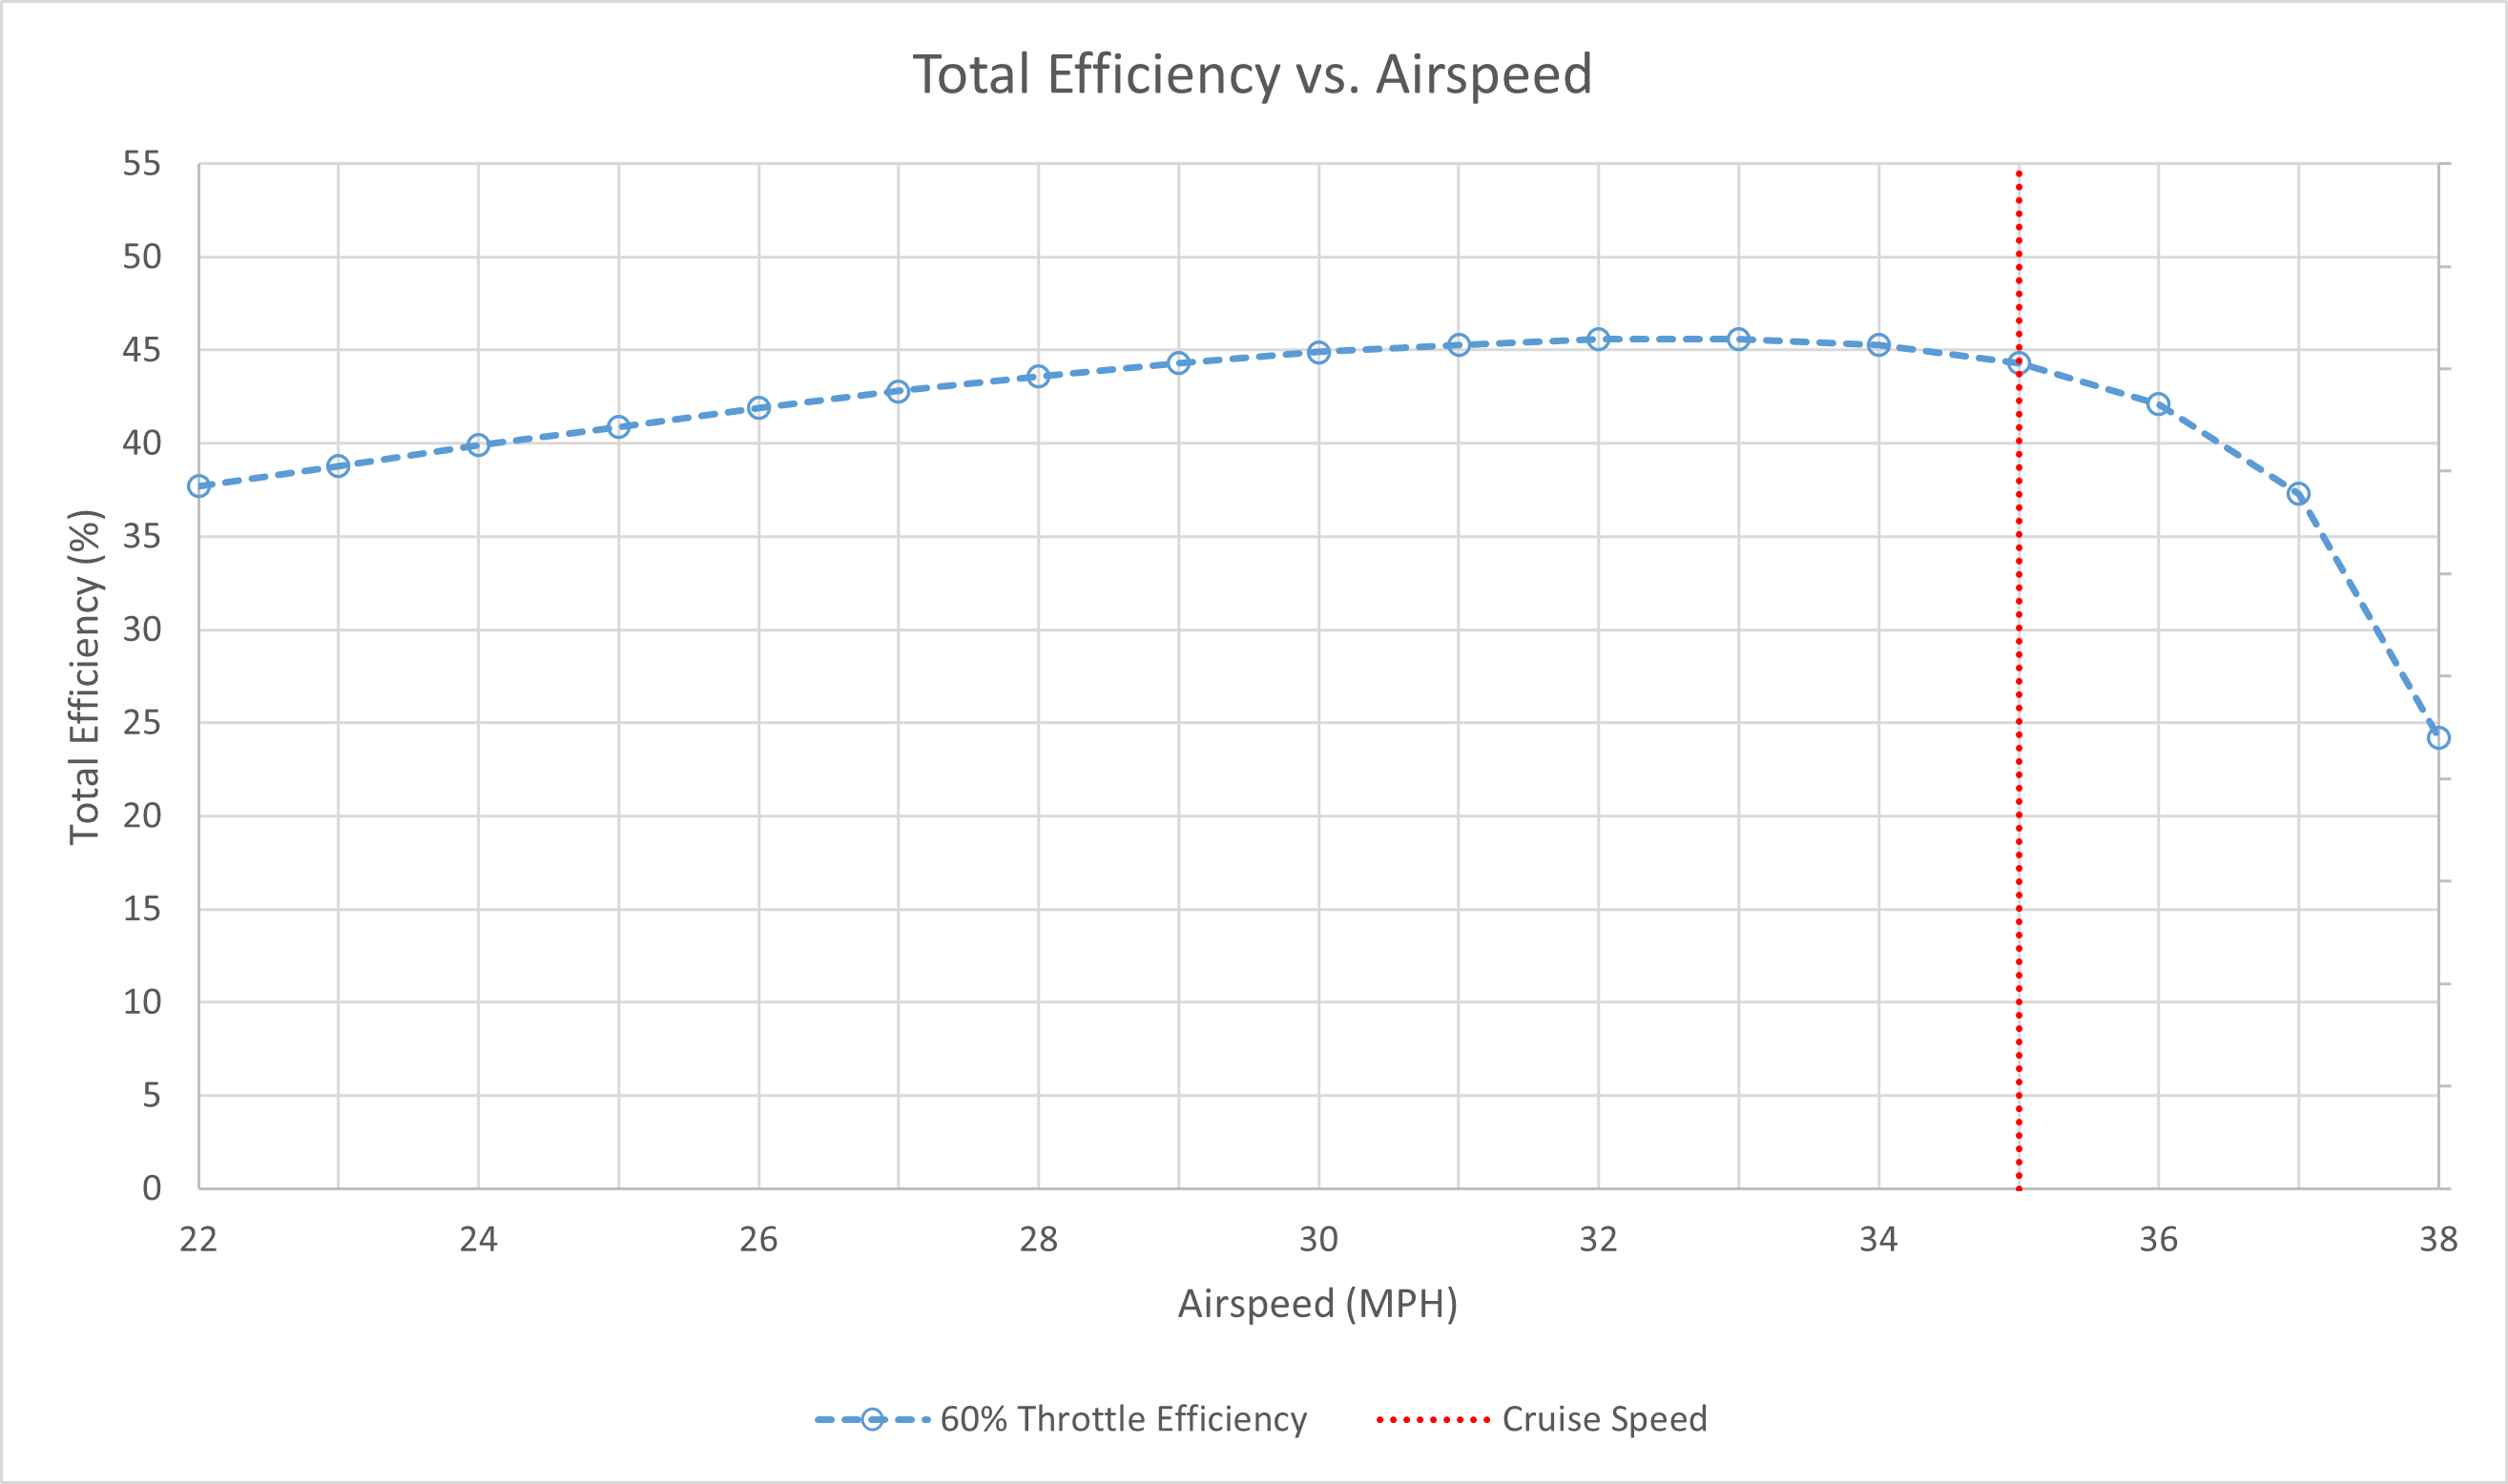
\includegraphics[width=\linewidth]{figures/eff_vs_airspeed.png}
    \end{frame}

    \begin{frame}{Current Propulsion System IV}
        \centering
        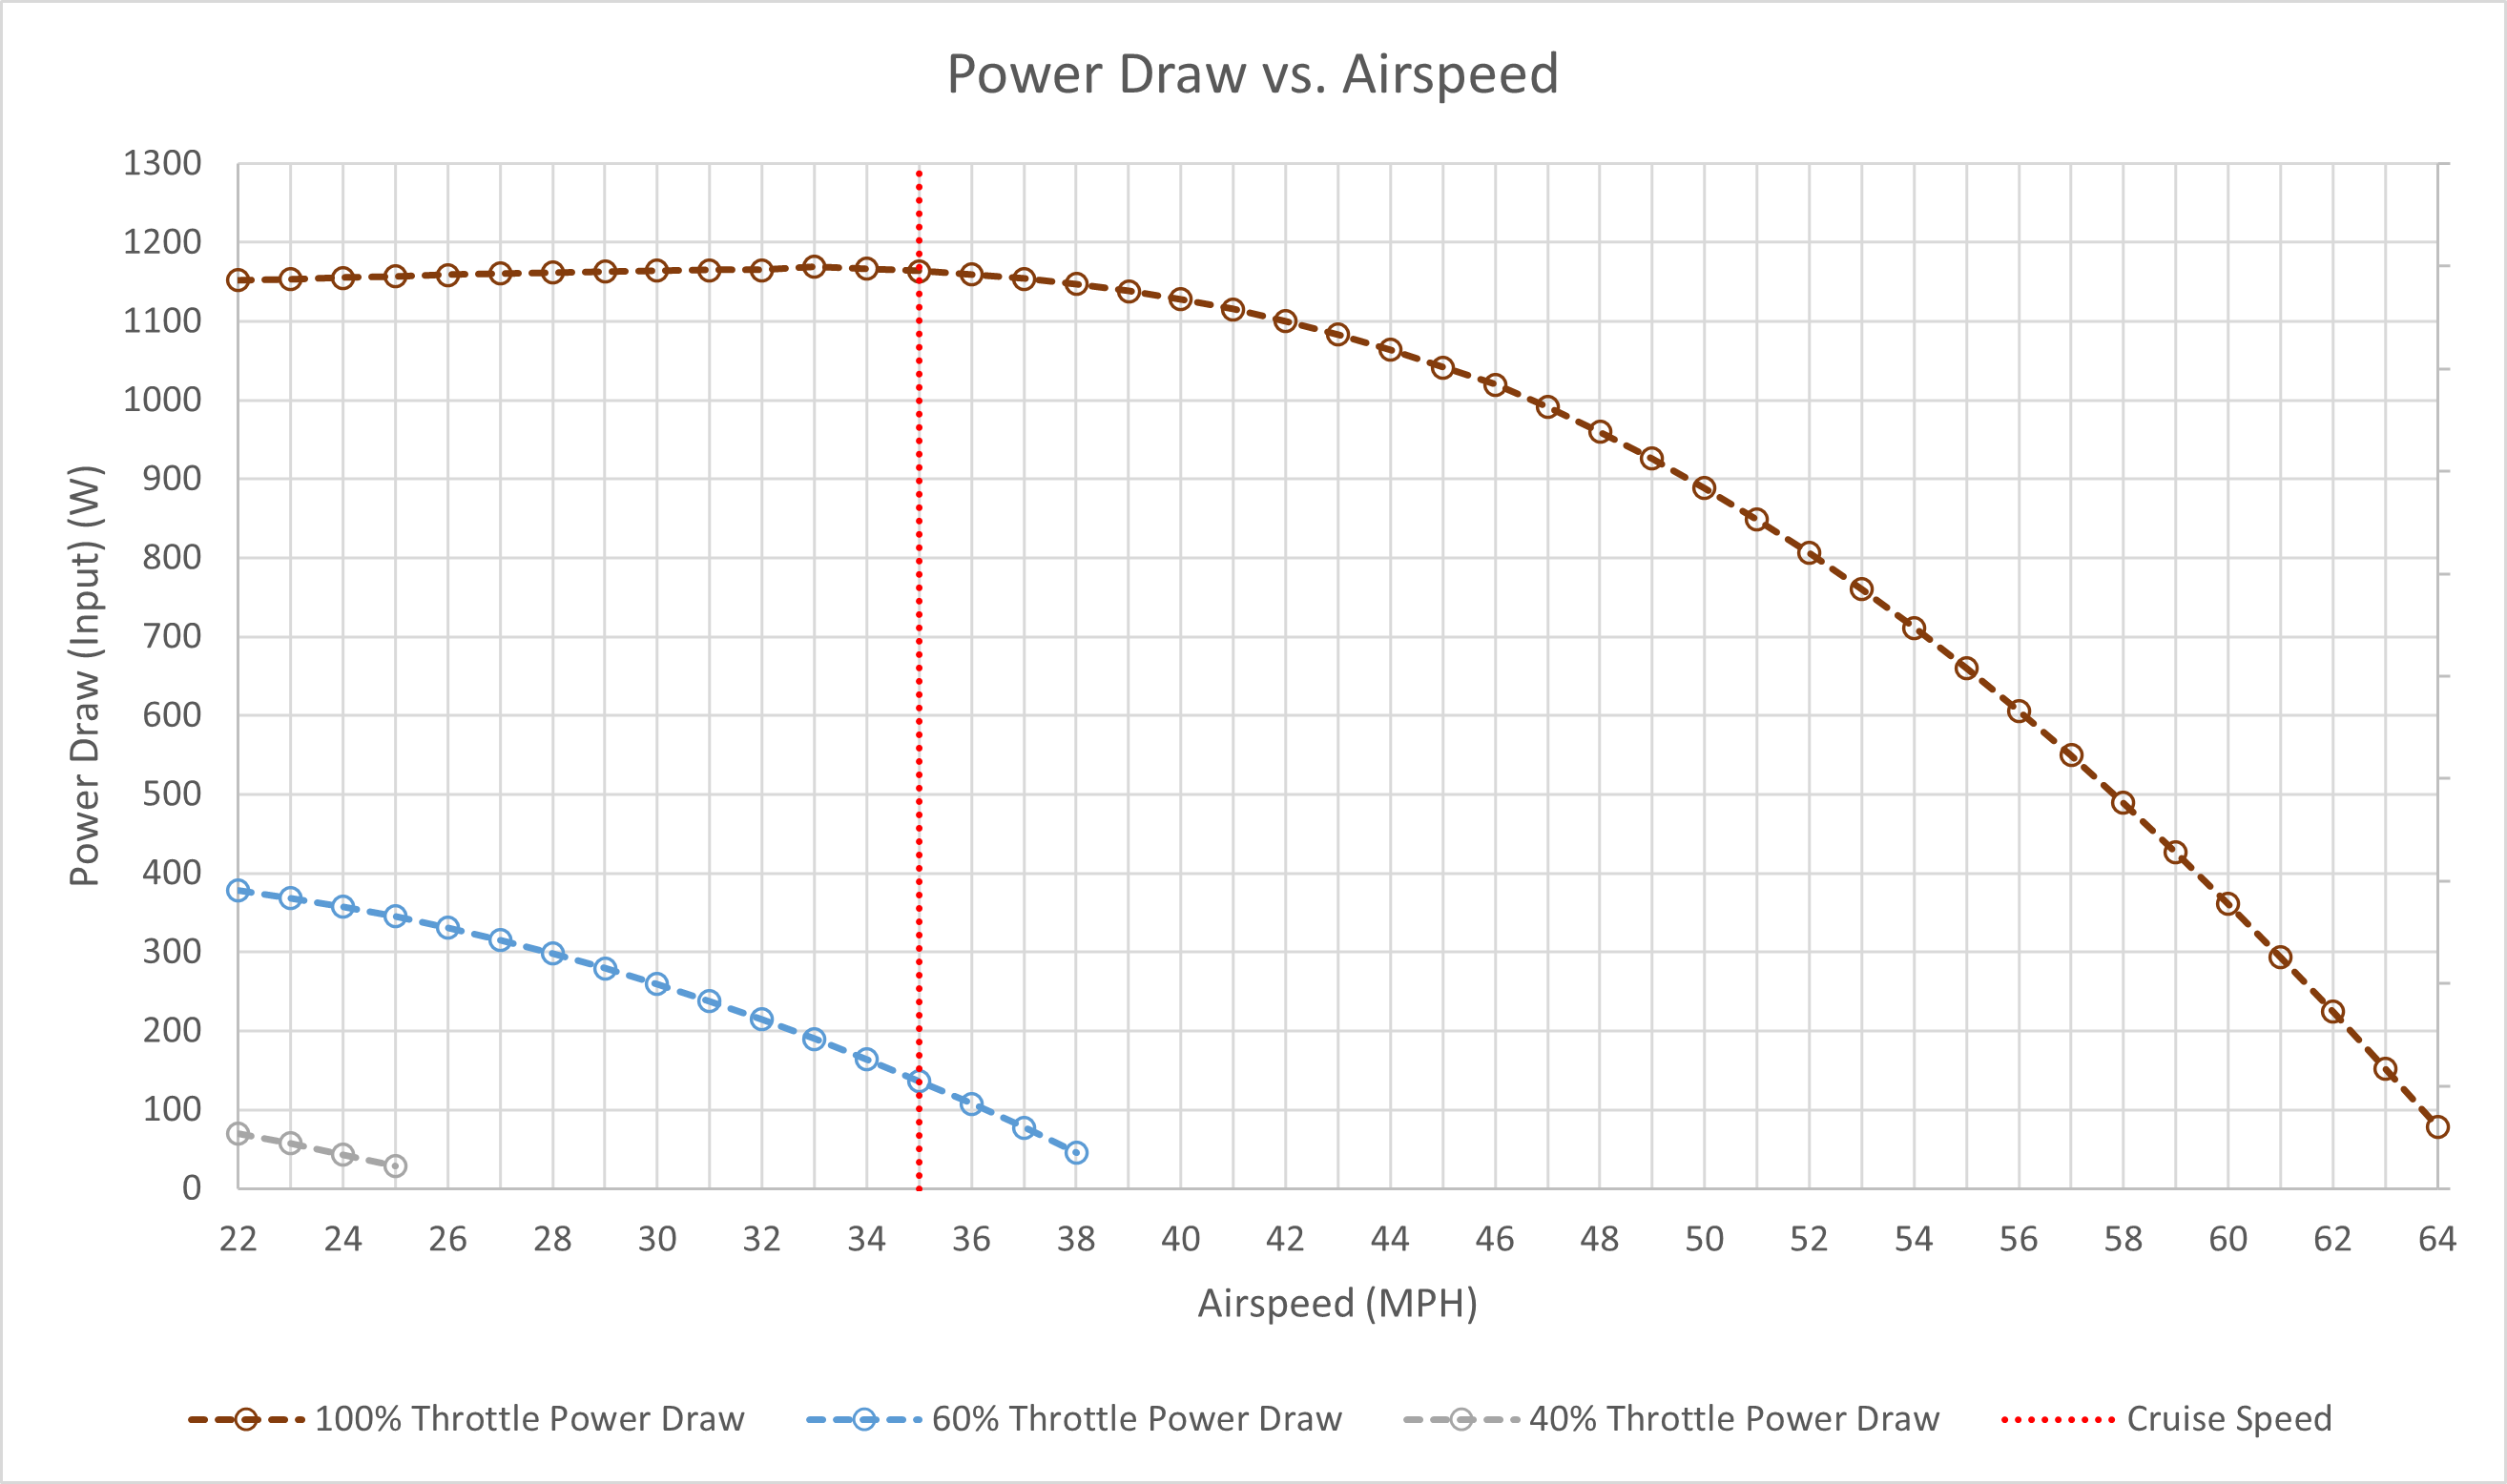
\includegraphics[width=1\linewidth]{figures/powerDraw_vs_airspeed.png}
    \end{frame}

    \subsection{Structures}

    \setpresentername{Ethan Witt}
    \setpresentertitle{Lead Structural Engineer}

    \begin{frame}{Structures I} % Going over initial spar selection assuming 2 identical spars per wing
        \begin{figure}[htbp]
            \centering
            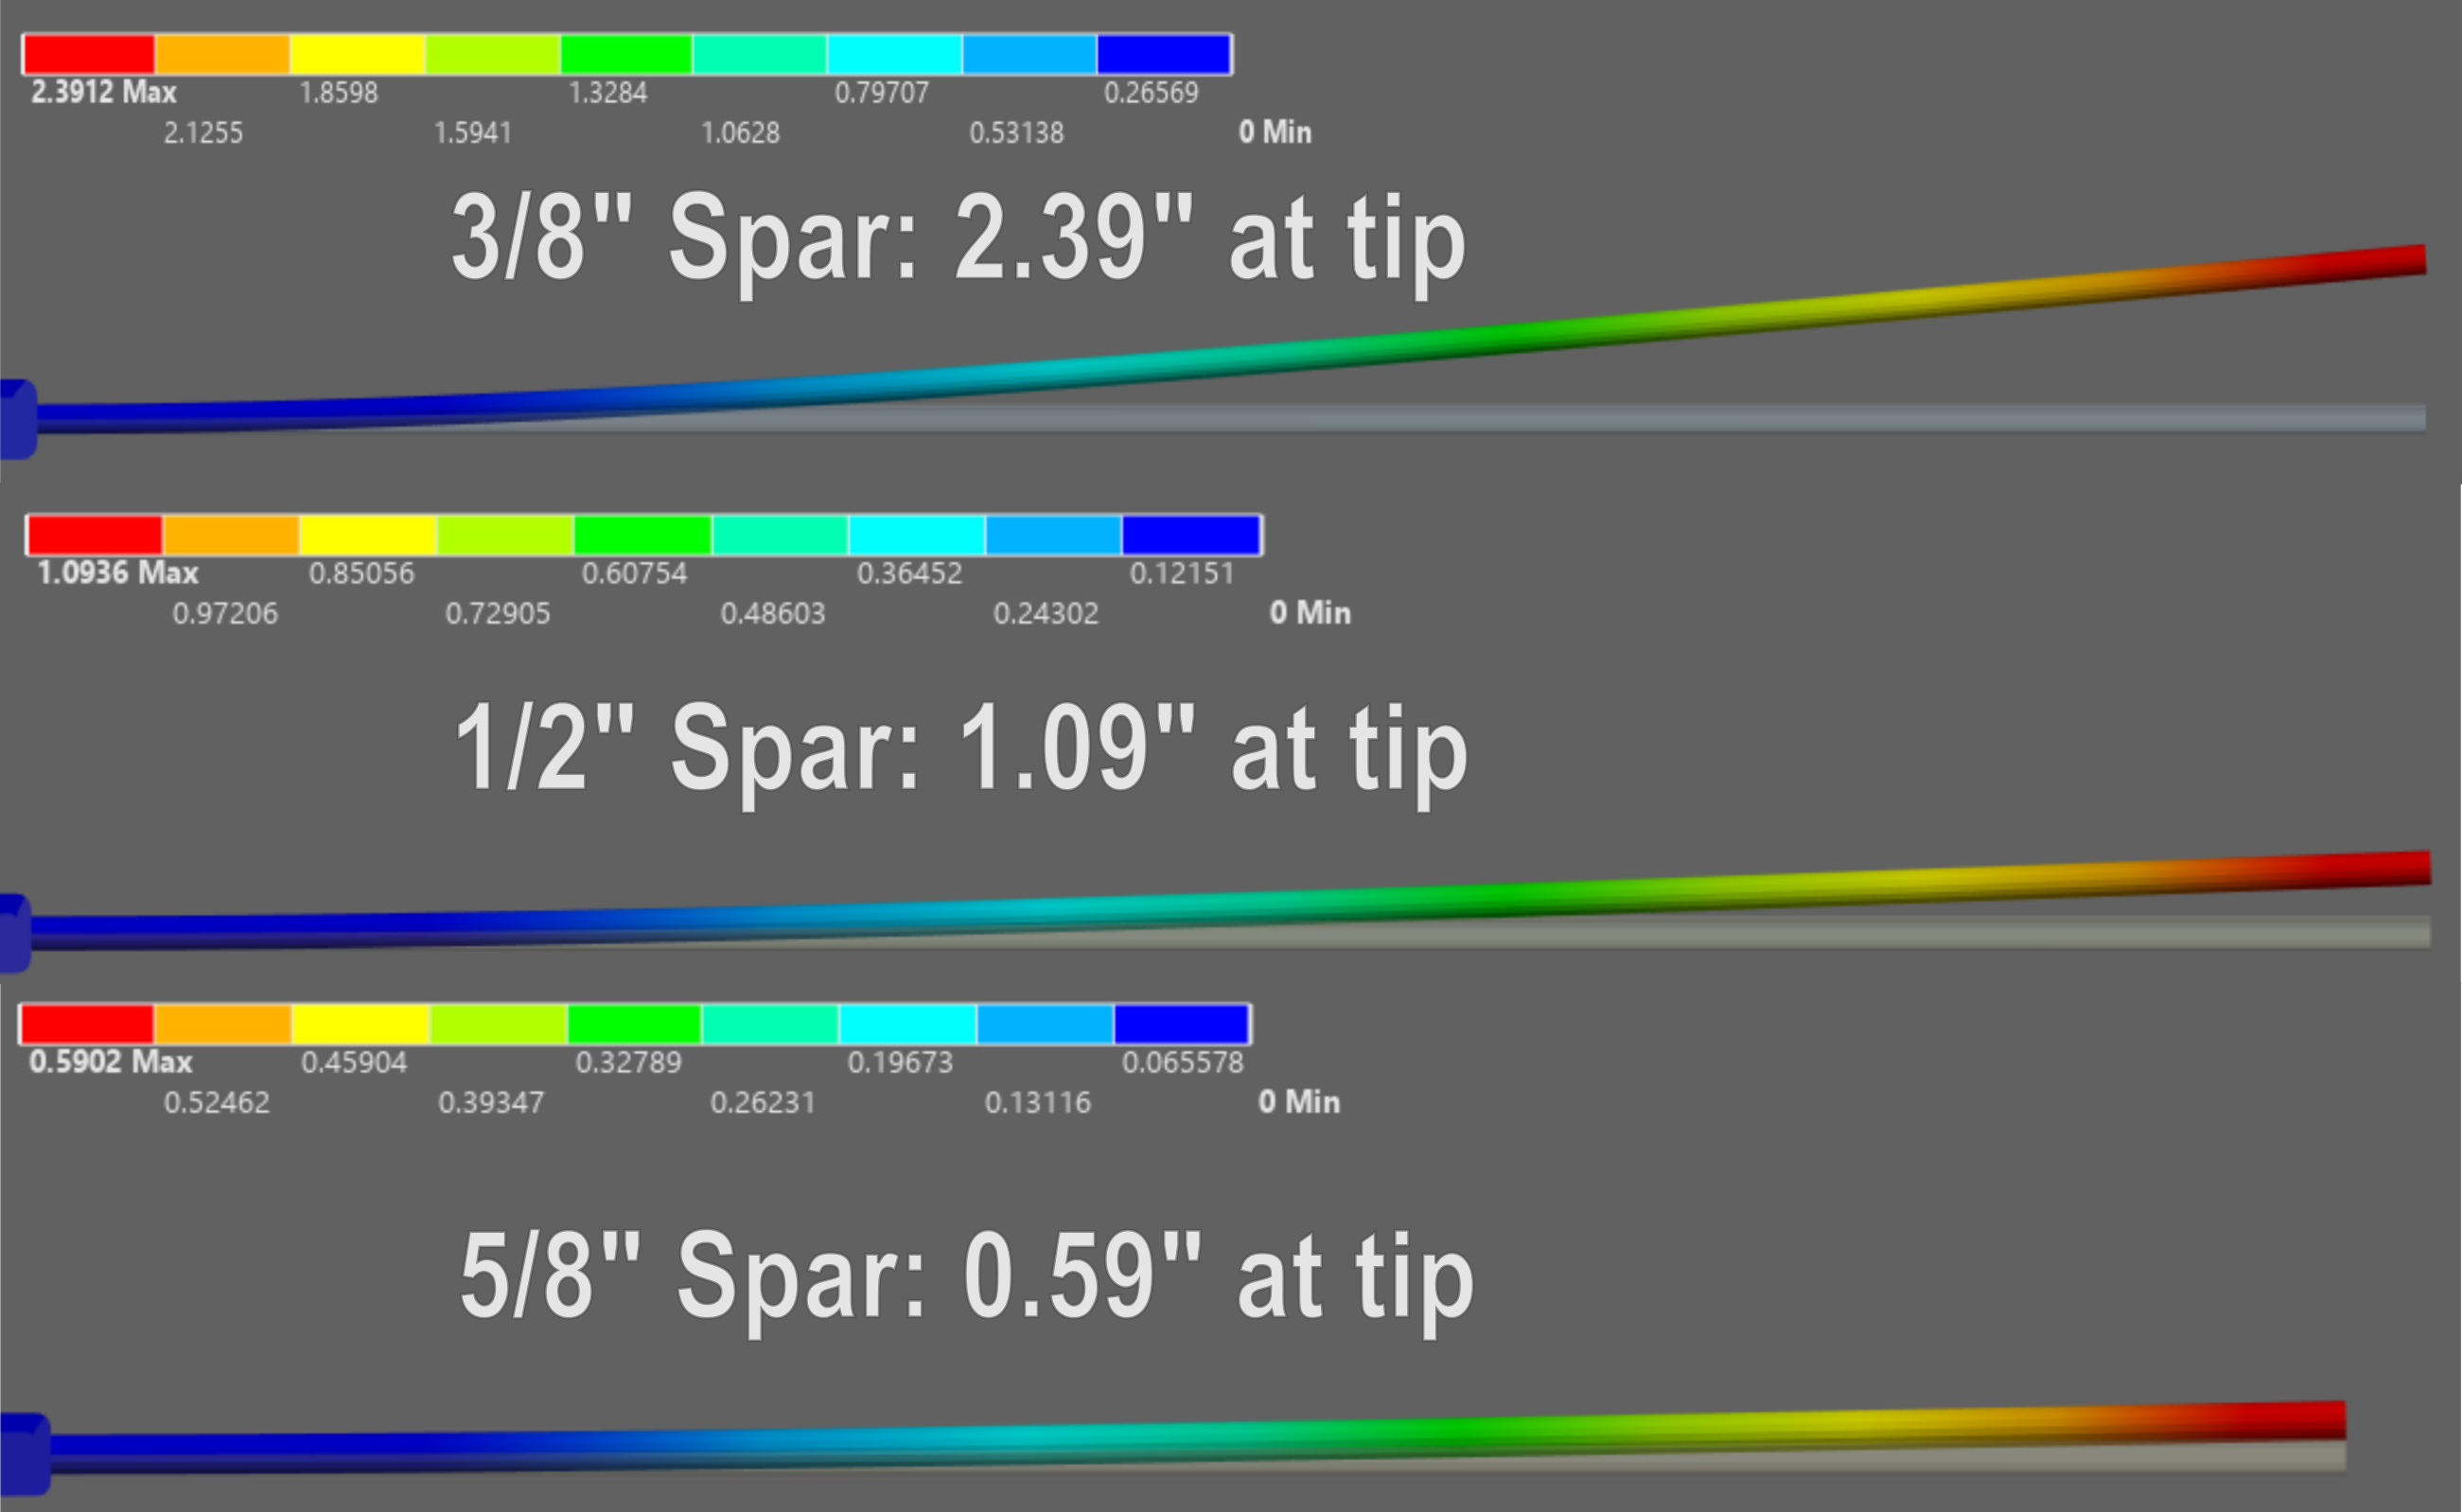
\includegraphics[width=\textwidth]{figures/Structures I Conglomerate.png}
        \end{figure}
    \end{frame}

    \begin{frame}{Structures II} % Going over spar differentiation assuming a smaller rear spar, and a more realistic load application (3G Elliptical Distribution)
        \begin{figure}[htbp]
            \centering
            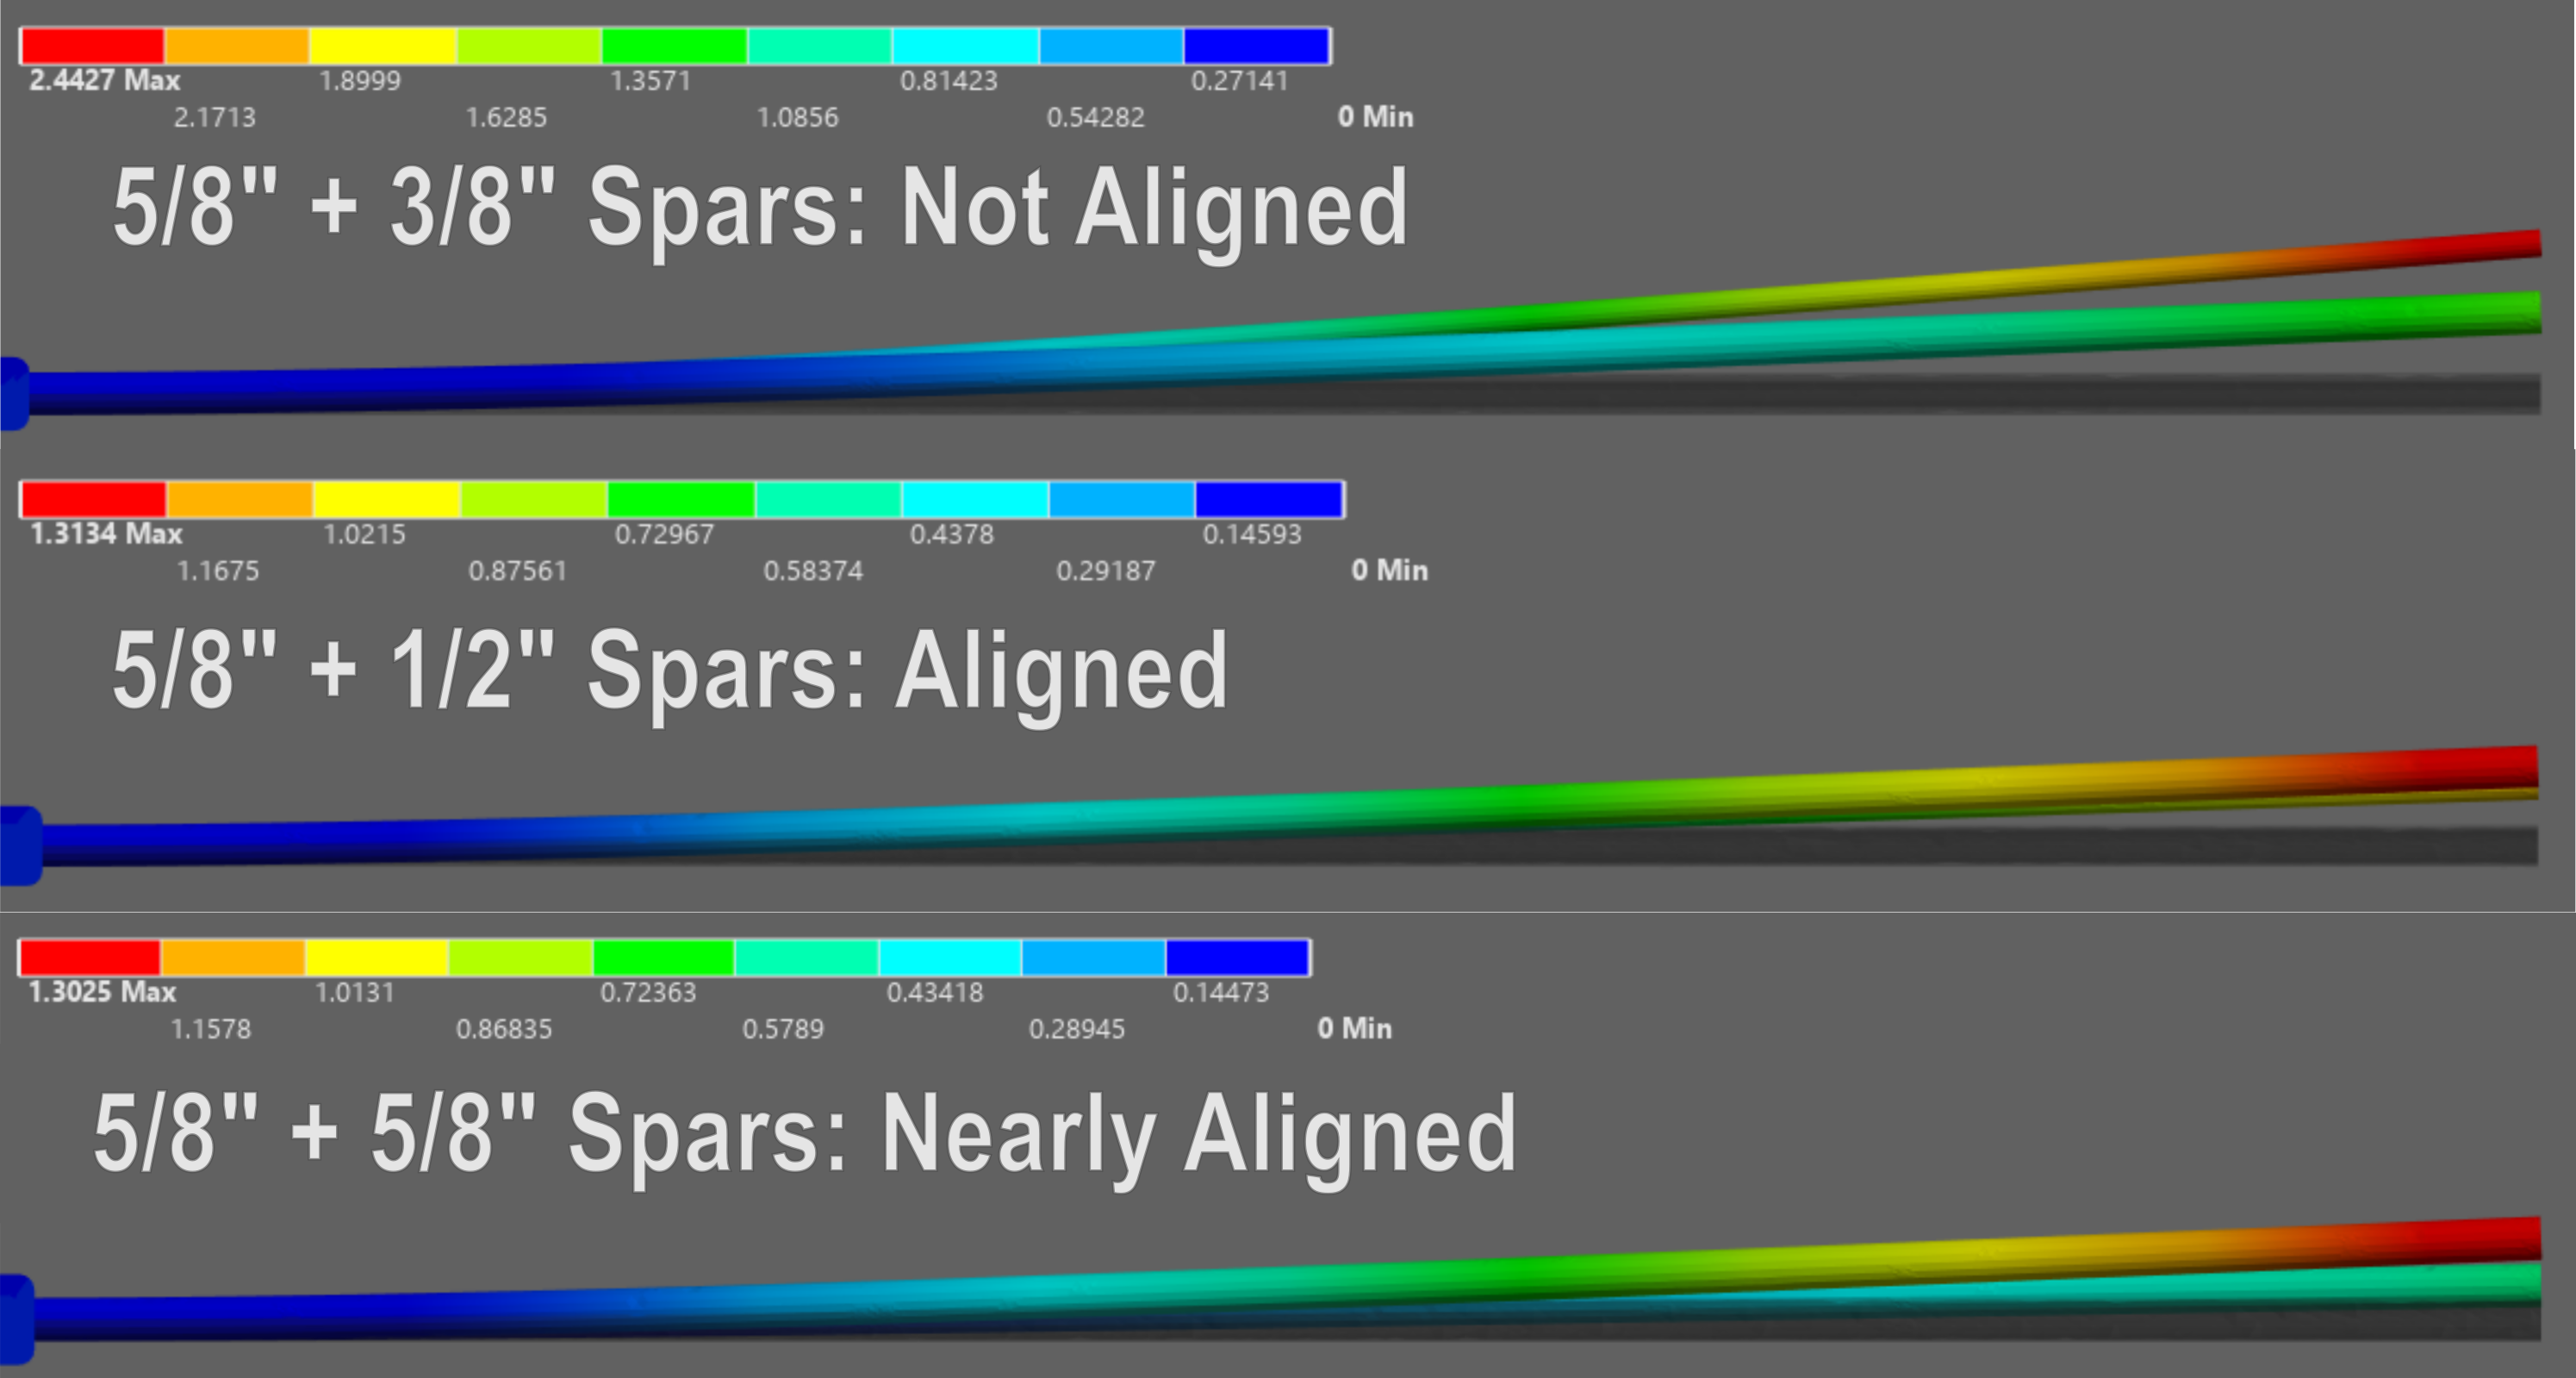
\includegraphics[width=\textwidth]{figures/Structures II Conglomerate.png}
        \end{figure}
    \end{frame}

    \begin{frame}{Structures III} % Going over final structural design and load distribution diagram
        \begin{figure}[htbp]
            \centering
            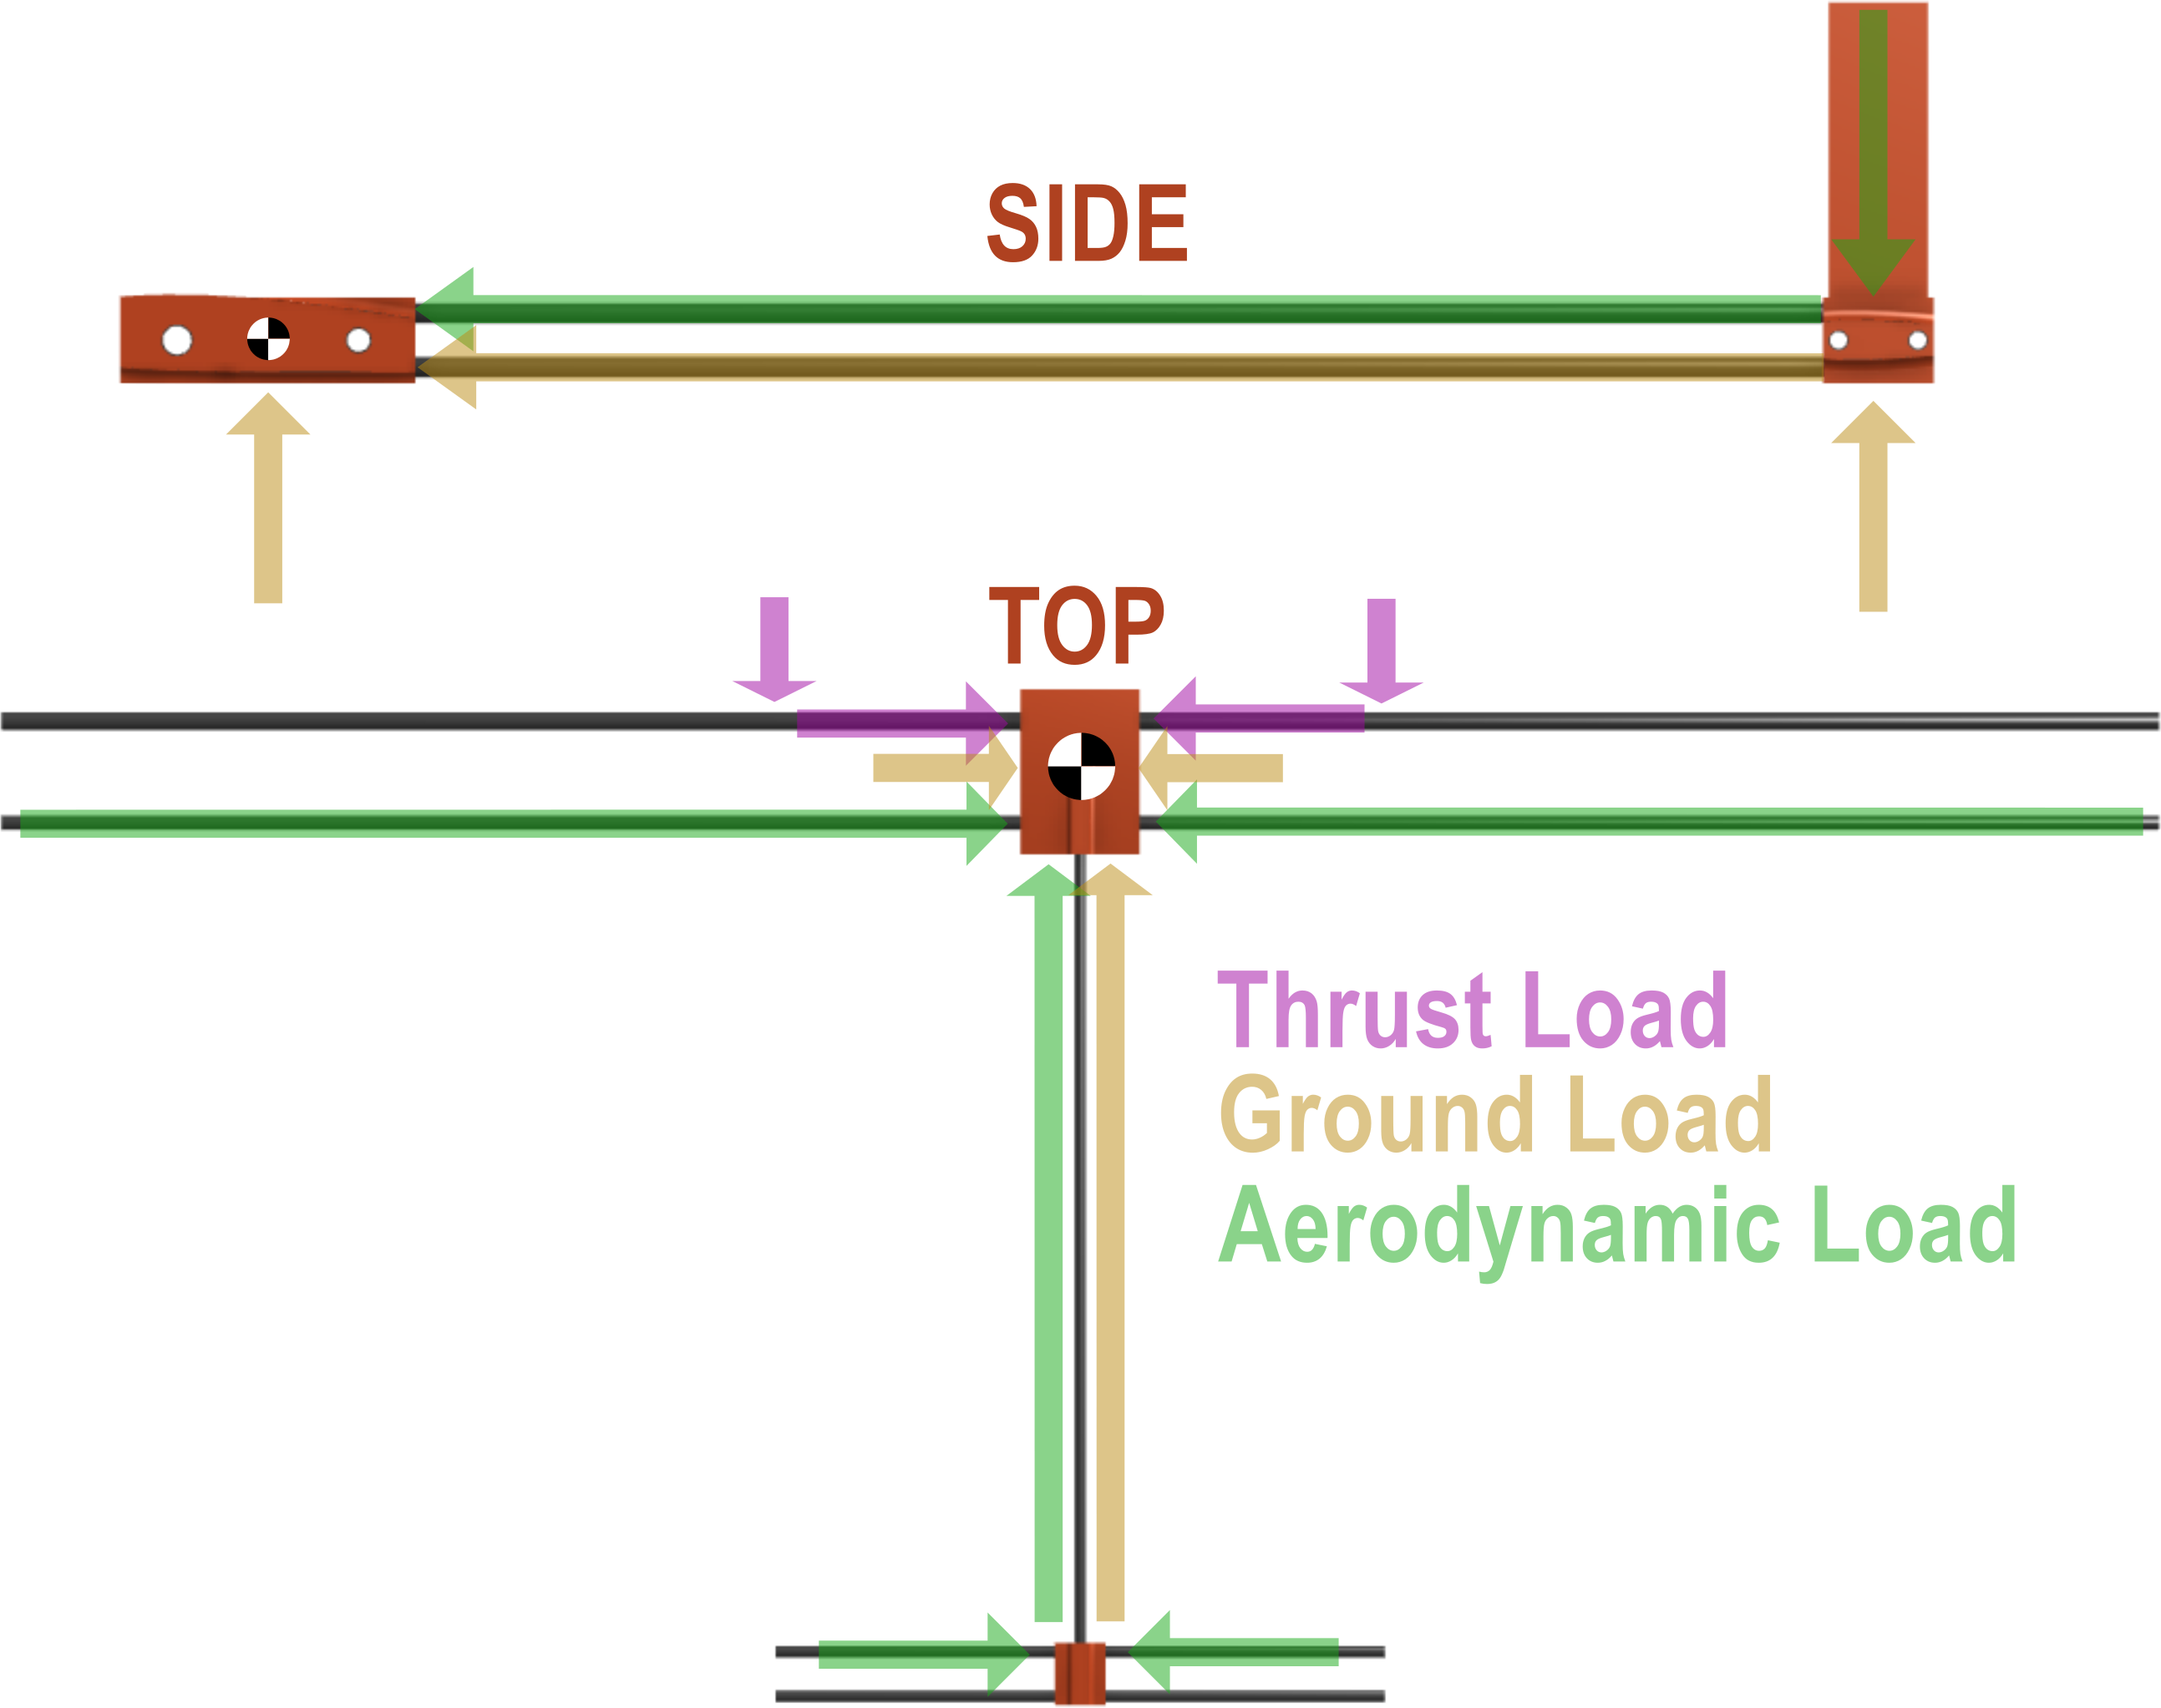
\includegraphics[width=0.97\textwidth]{figures/Structures III Load Map.png}
        \end{figure}
    \end{frame}

    \section{Current Concept}
    \setpresentername{Bradley Nordwall}
    \setpresentertitle{Lead CAD Engineer}
    \begin{frame}{Aircraft Progression}
        \begin{columns}[T]
            \begin{column}{0.5\textwidth}
                \centering
                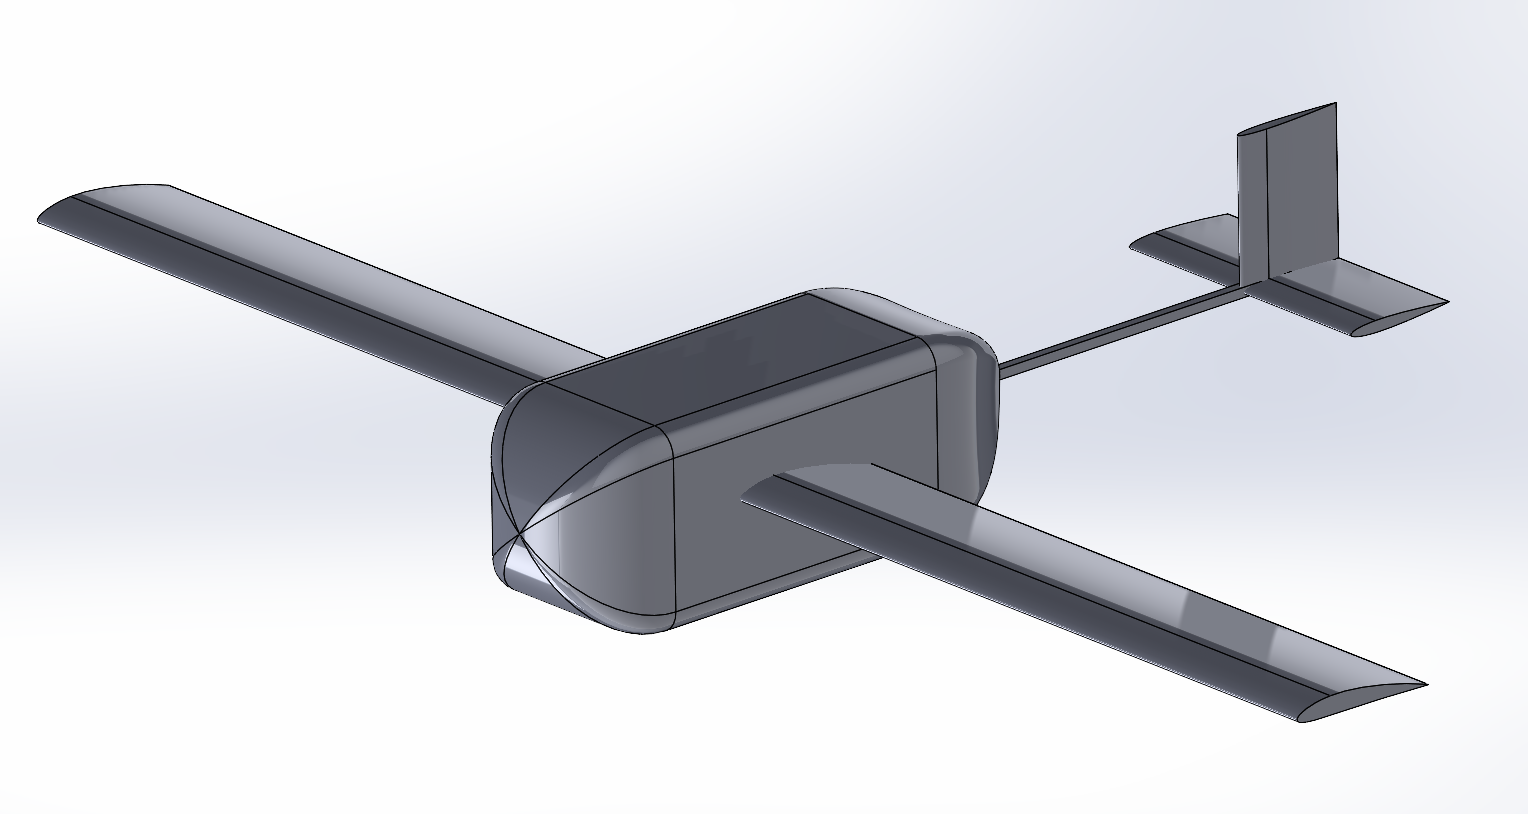
\includegraphics[width=\textwidth]{figures/isometrics over time/Assem1.0.1Iso.png}
                \vspace{0.5em} % Space between image and caption
                \text{Initial Design}
            \end{column}
    
            \begin{column}{0.5\textwidth}
                \centering
                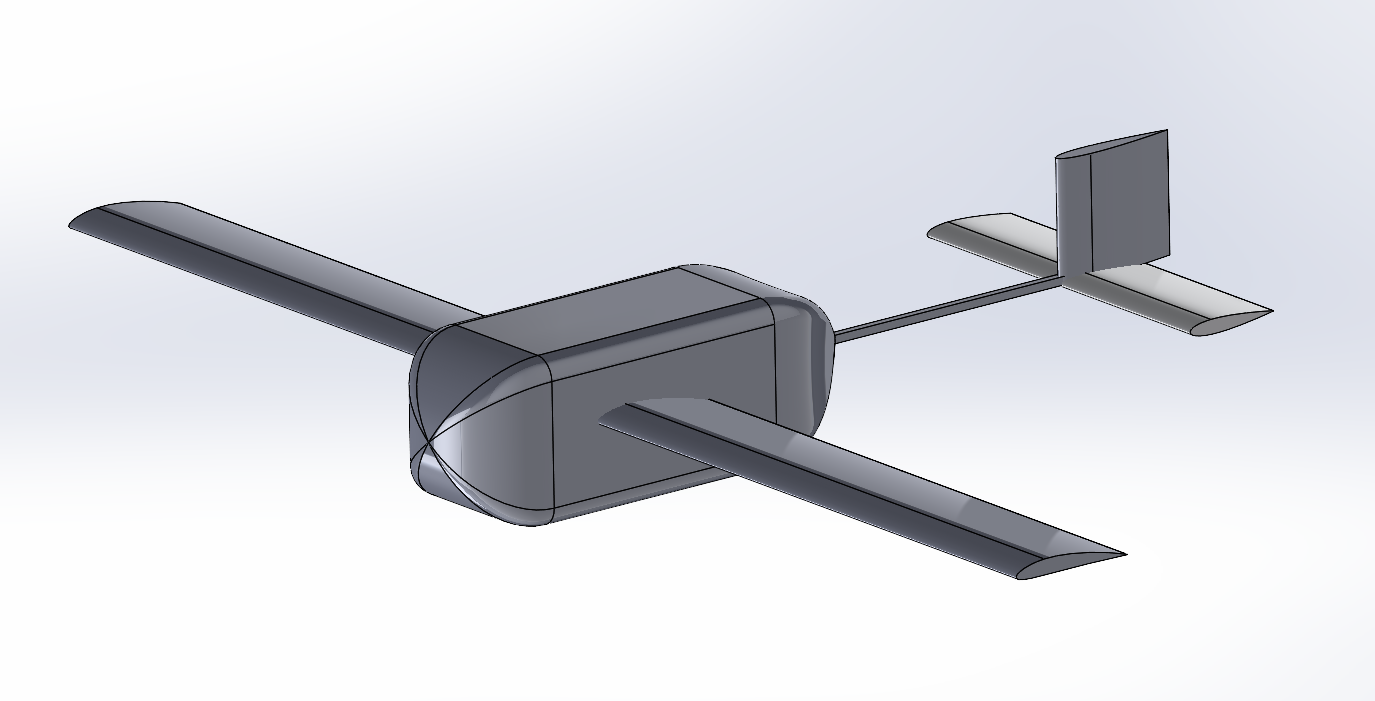
\includegraphics[width=\textwidth]{figures/isometrics over time/Assem1.1.12Iso.png}
                \vspace{0.5em} % Space between image and caption
                \text{Iteration 1}
            \end{column}
        \end{columns}
    
        \vspace{1em}
    
        \begin{columns}[T]
            \begin{column}{0.5\textwidth}
                \centering
                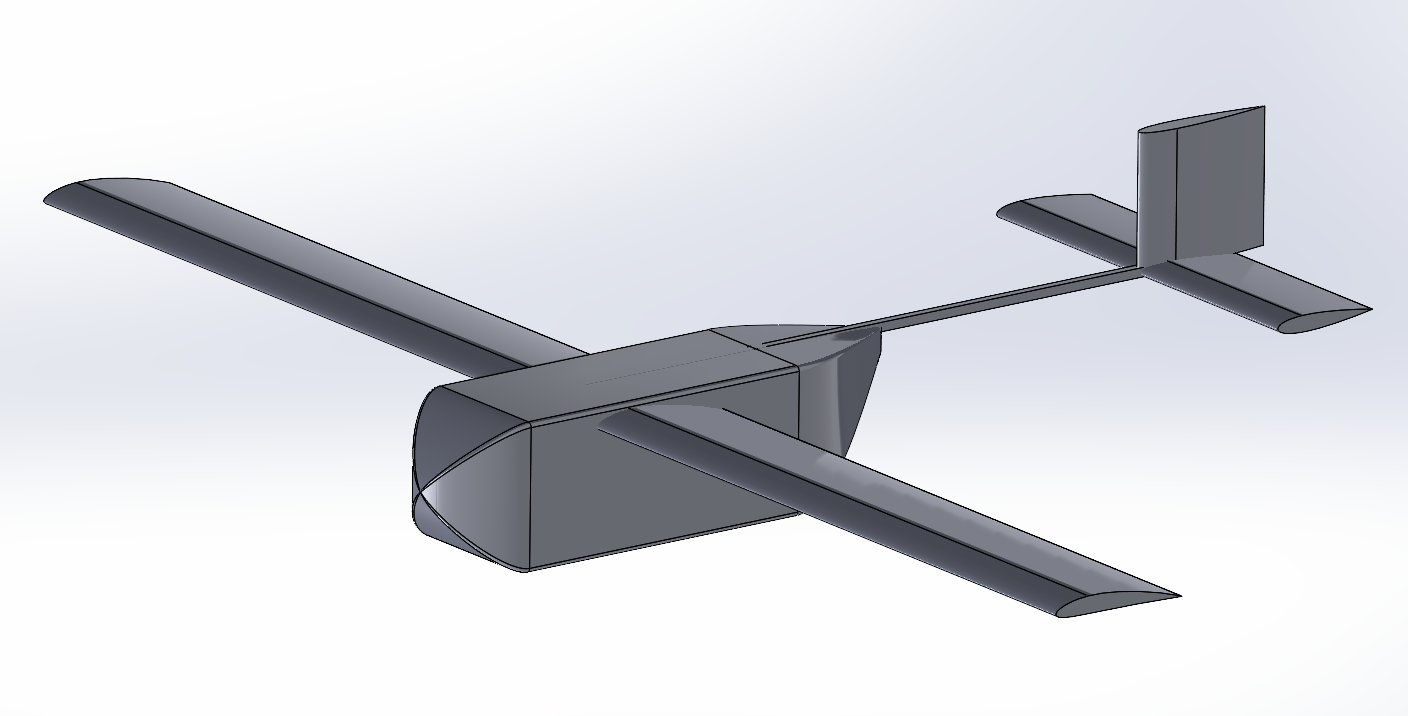
\includegraphics[width=\textwidth]{figures/isometrics over time/Assem2.0.0Iso.png}
                \vspace{0.5em} % Space between image and caption
                \text{Iteration 2}
            \end{column}
    
            \begin{column}{0.5\textwidth}
                \centering
                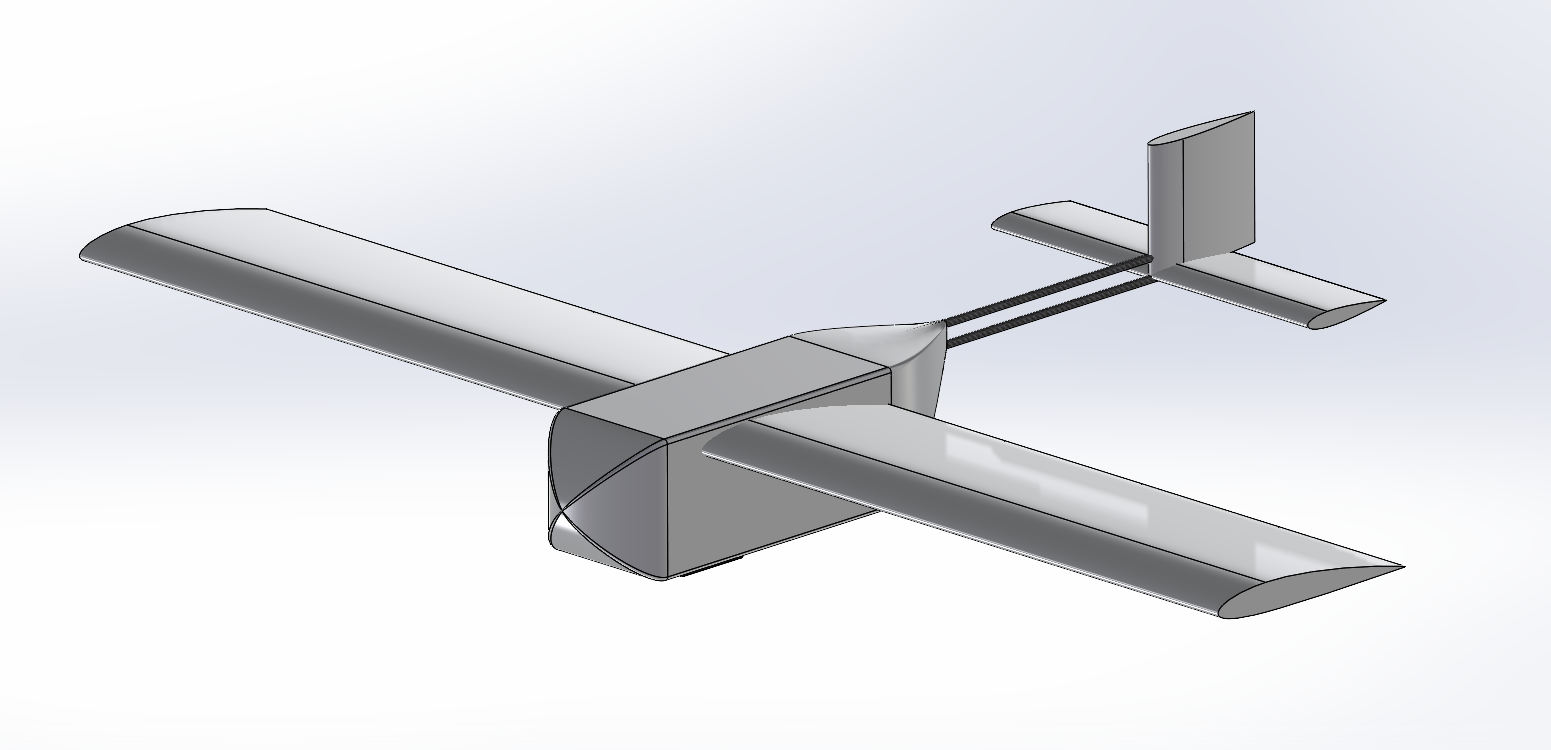
\includegraphics[width=\textwidth]{figures/isometrics over time/Assem3.0.0Iso.png}
                \vspace{0.5em} % Space between image and caption
                \text{Iteration 3}
            \end{column}
        \end{columns}
    \end{frame}

    \begin{frame}{Current Aircraft I}
        \centering
        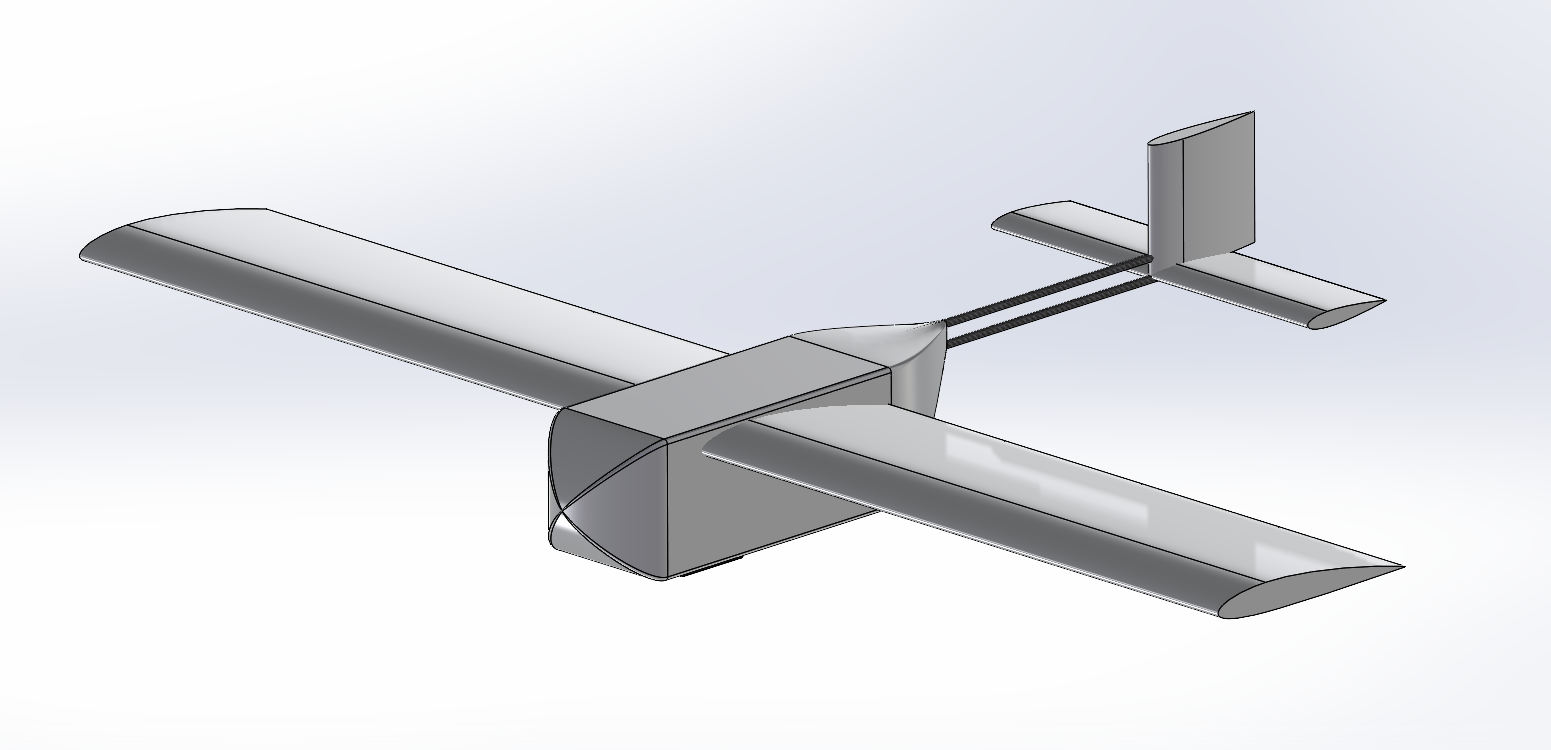
\includegraphics[width=\textwidth]{figures/current/Current Iso.png}
    \end{frame}

    \begin{frame}{Current Aircraft II}
        \begin{columns}[T]
            \begin{column}{0.5\textwidth}
                \centering
                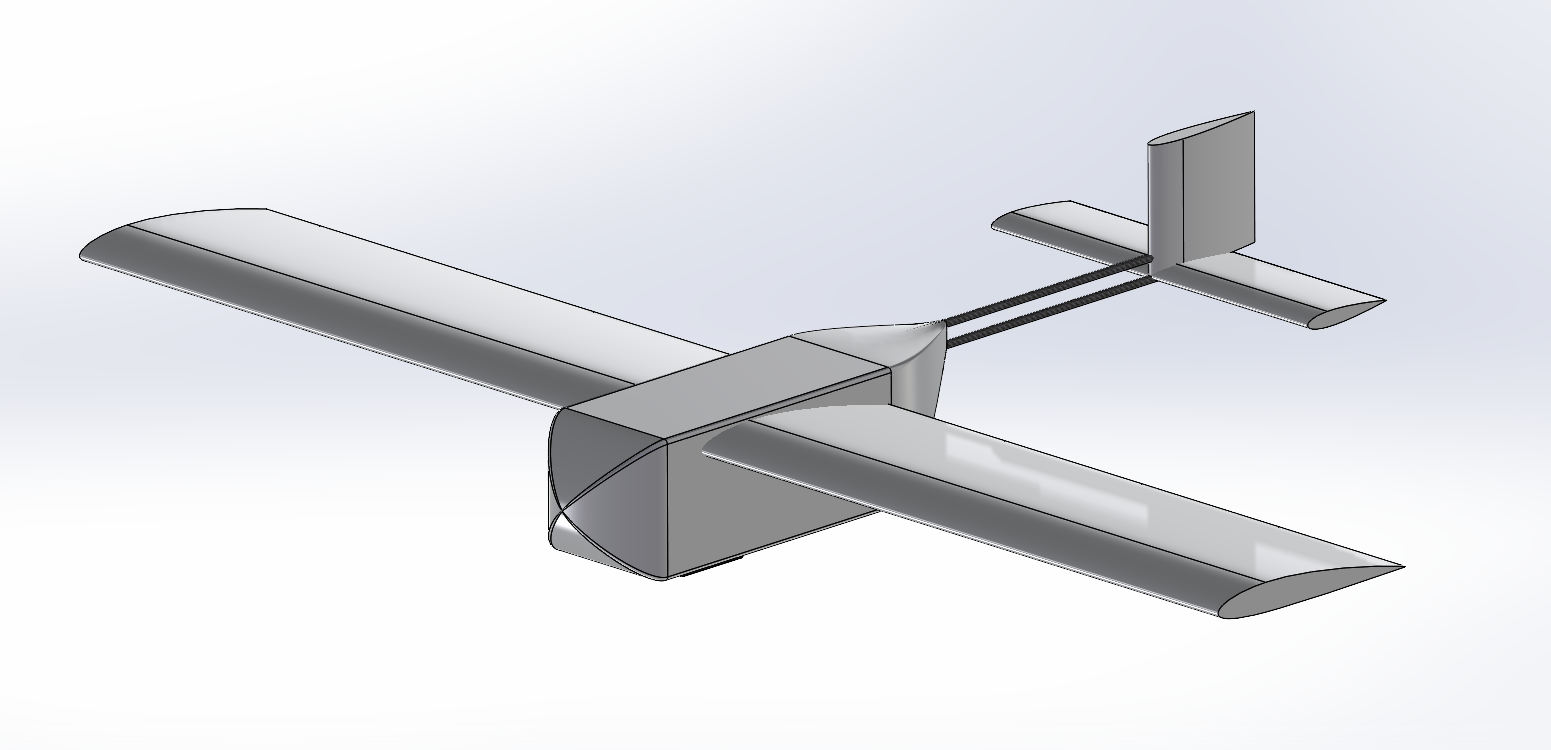
\includegraphics[width=\textwidth]{figures/current/Current Iso.png}
            \end{column}
    
            \begin{column}{0.5\textwidth}
                \centering
                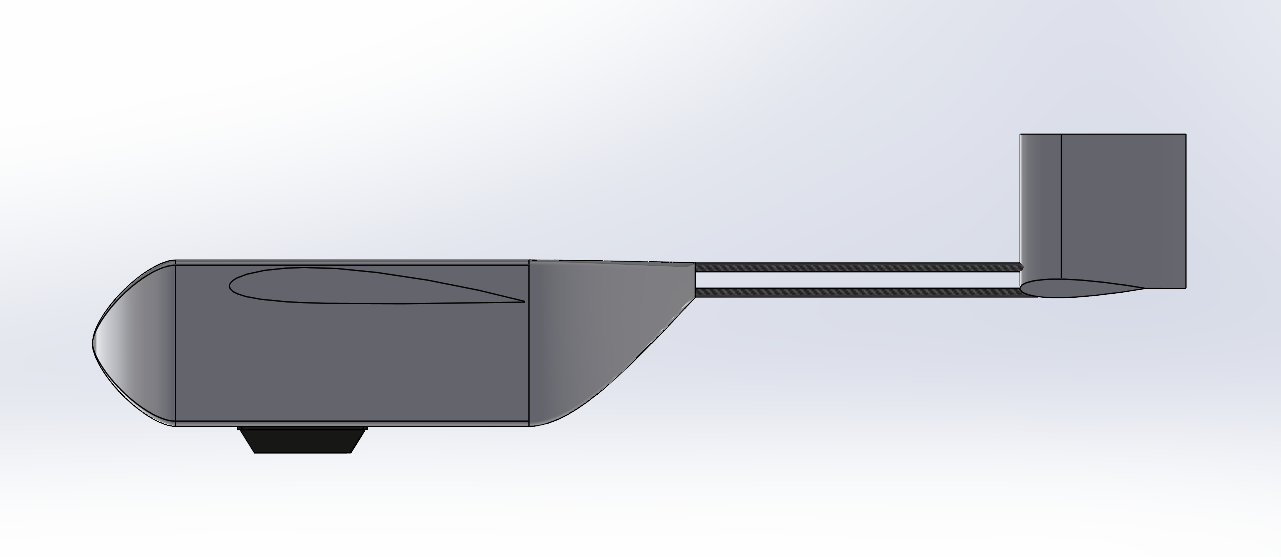
\includegraphics[width=\textwidth]{figures/current/Current Side.png}
            \end{column}
        \end{columns}
    
        \vspace{1em}
    
        \begin{columns}[T]
            \begin{column}{0.5\textwidth}
                \centering
                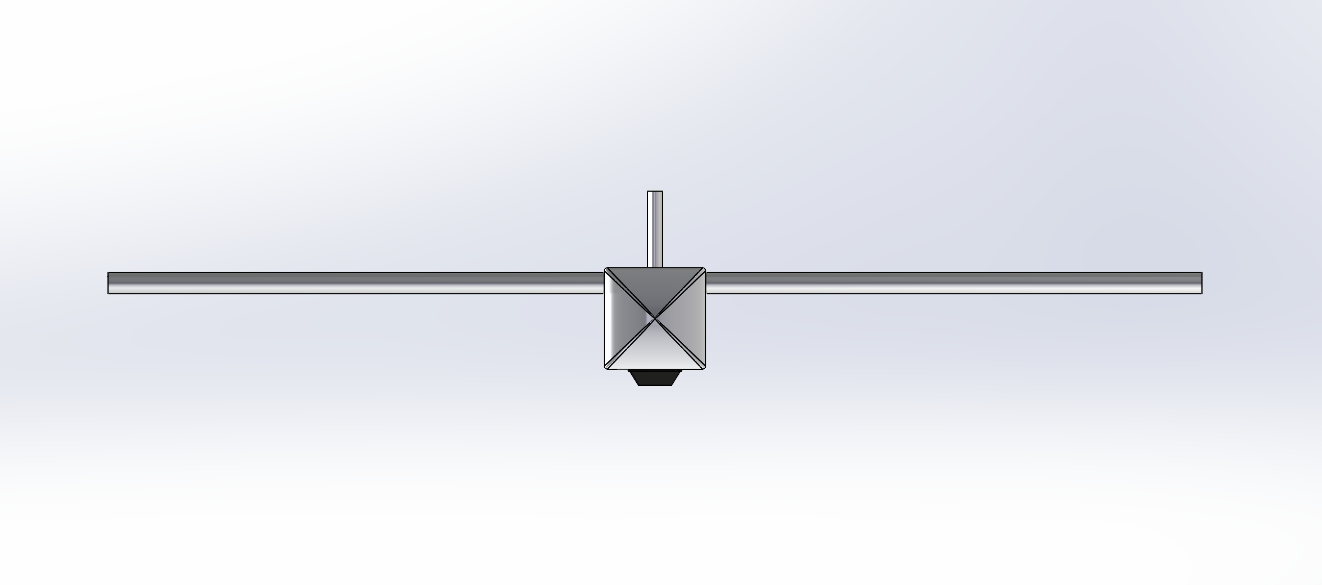
\includegraphics[width=\textwidth]{figures/current/Current Front.png}
            \end{column}
    
            \begin{column}{0.5\textwidth}
                \centering
                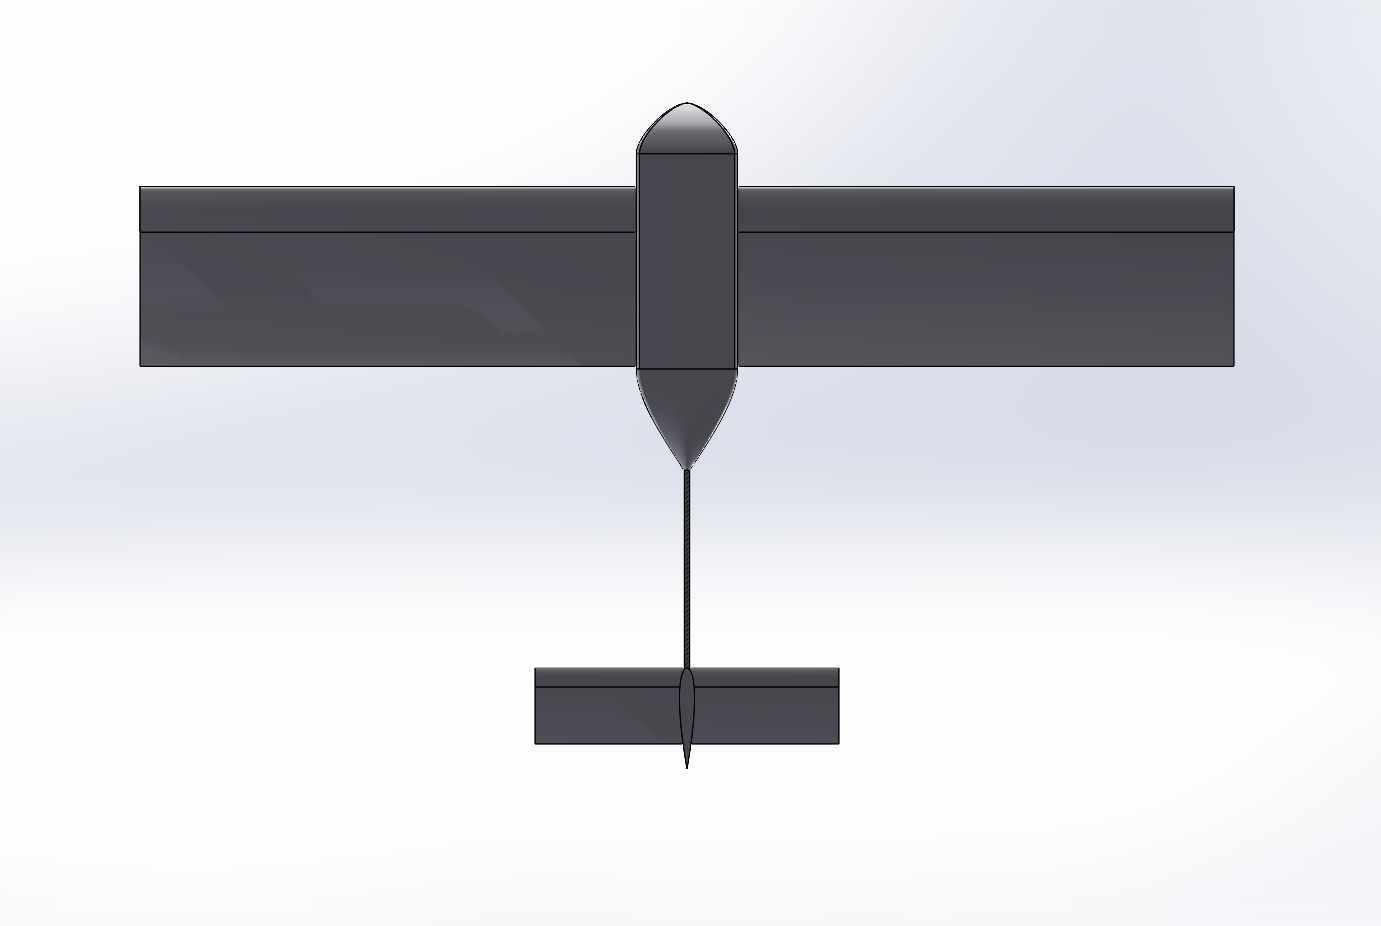
\includegraphics[width=\textwidth]{figures/current/Current Top.png}
            \end{column}
        \end{columns}
    \end{frame}

    \setpresentername{Patricia Ovono}
    \setpresentertitle{Flight Performance Engineer}
    \begin{frame}{Internal Components}
        \centering
        \includegraphics[width=\textwidth]{figures/box internals/InternalsAndBox.jpg}    
    \end{frame}

    \begin{frame}{Internal Concept}
        \centering
        \includegraphics[width=\textwidth]{figures/box internals/BoxInFuselage.jpg}
    \end{frame}

    \begin{frame}{Dimensions}
        \centering
        \includegraphics[width=\textwidth]{figures/current/Current Dimensions.png}
        \vspace{0.5em} % Space between image and caption
        Estimated Weight: \qty{6.38}{lbs}
    \end{frame}

    \section{Conclusion}

    \setpresentername{Matthew Mehrtens}
    \setpresentertitle{Project Manager}

    \begin{frame}{Next Steps}
        \begin{enumerate}
            \item Finalize requirements and system scorecard
            \item Design control surfaces
            \item Design landing gear
            \item Refine CAD design
            \item Create a BOM
            \item Create manufacturing plan
        \end{enumerate}
    \end{frame}

    \begin{frame}{Closing Summary}
        \begin{enumerate}
            \item<2-> Unique versatility not found in the market
            \item<3-> Cost effective
            \item<4-> Design headroom
        \end{enumerate}
        \vspace{10pt}
        \centering
        \includegraphics<1->[width=\textwidth]{figures/current/Current Iso.png}
    \end{frame}

    \appendix

    \section*{Appendix Contents}

    \showpresenterboxfalse
    \showheadlinefalse

    \begin{frame}{Appendix Contents}
        \tableofcontents
    \end{frame}

    \section{Longitudinal Stability}

    \begin{frame}{Longitudinal Stability}
        \centering
        \begin{figure}
            \includegraphics[width=\textwidth]{figures/currentiterationCGNP.png}
            \caption{CG and NP on current design iteration.}
        \end{figure}
    \end{frame}
\end{document}
